\documentclass[twoside]{book}

% Packages required by doxygen
\usepackage{fixltx2e}
\usepackage{calc}
\usepackage{doxygen}
\usepackage[export]{adjustbox} % also loads graphicx
\usepackage{graphicx}
\usepackage[utf8]{inputenc}
\usepackage{makeidx}
\usepackage{multicol}
\usepackage{multirow}
\PassOptionsToPackage{warn}{textcomp}
\usepackage{textcomp}
\usepackage[nointegrals]{wasysym}
\usepackage[table]{xcolor}

% Font selection
\usepackage[T1]{fontenc}
\usepackage[scaled=.90]{helvet}
\usepackage{courier}
\usepackage{amssymb}
\usepackage{sectsty}
\renewcommand{\familydefault}{\sfdefault}
\allsectionsfont{%
  \fontseries{bc}\selectfont%
  \color{darkgray}%
}
\renewcommand{\DoxyLabelFont}{%
  \fontseries{bc}\selectfont%
  \color{darkgray}%
}
\newcommand{\+}{\discretionary{\mbox{\scriptsize$\hookleftarrow$}}{}{}}

% Page & text layout
\usepackage{geometry}
\geometry{%
  a4paper,%
  top=2.5cm,%
  bottom=2.5cm,%
  left=2.5cm,%
  right=2.5cm%
}
\tolerance=750
\hfuzz=15pt
\hbadness=750
\setlength{\emergencystretch}{15pt}
\setlength{\parindent}{0cm}
\setlength{\parskip}{3ex plus 2ex minus 2ex}
\makeatletter
\renewcommand{\paragraph}{%
  \@startsection{paragraph}{4}{0ex}{-1.0ex}{1.0ex}{%
    \normalfont\normalsize\bfseries\SS@parafont%
  }%
}
\renewcommand{\subparagraph}{%
  \@startsection{subparagraph}{5}{0ex}{-1.0ex}{1.0ex}{%
    \normalfont\normalsize\bfseries\SS@subparafont%
  }%
}
\makeatother

% Headers & footers
\usepackage{fancyhdr}
\pagestyle{fancyplain}
\fancyhead[LE]{\fancyplain{}{\bfseries\thepage}}
\fancyhead[CE]{\fancyplain{}{}}
\fancyhead[RE]{\fancyplain{}{\bfseries\leftmark}}
\fancyhead[LO]{\fancyplain{}{\bfseries\rightmark}}
\fancyhead[CO]{\fancyplain{}{}}
\fancyhead[RO]{\fancyplain{}{\bfseries\thepage}}
\fancyfoot[LE]{\fancyplain{}{}}
\fancyfoot[CE]{\fancyplain{}{}}
\fancyfoot[RE]{\fancyplain{}{\bfseries\scriptsize Generated by Doxygen }}
\fancyfoot[LO]{\fancyplain{}{\bfseries\scriptsize Generated by Doxygen }}
\fancyfoot[CO]{\fancyplain{}{}}
\fancyfoot[RO]{\fancyplain{}{}}
\renewcommand{\footrulewidth}{0.4pt}
\renewcommand{\chaptermark}[1]{%
  \markboth{#1}{}%
}
\renewcommand{\sectionmark}[1]{%
  \markright{\thesection\ #1}%
}

% Indices & bibliography
\usepackage{natbib}
\usepackage[titles]{tocloft}
\setcounter{tocdepth}{3}
\setcounter{secnumdepth}{5}
\makeindex

% Hyperlinks (required, but should be loaded last)
\usepackage{ifpdf}
\ifpdf
  \usepackage[pdftex,pagebackref=true]{hyperref}
\else
  \usepackage[ps2pdf,pagebackref=true]{hyperref}
\fi
\hypersetup{%
  colorlinks=true,%
  linkcolor=blue,%
  citecolor=blue,%
  unicode%
}

% Custom commands
\newcommand{\clearemptydoublepage}{%
  \newpage{\pagestyle{empty}\cleardoublepage}%
}

\usepackage{caption}
\captionsetup{labelsep=space,justification=centering,font={bf},singlelinecheck=off,skip=4pt,position=top}

%===== C O N T E N T S =====

\begin{document}

% Titlepage & ToC
\hypersetup{pageanchor=false,
             bookmarksnumbered=true,
             pdfencoding=unicode
            }
\pagenumbering{roman}
\begin{titlepage}
\vspace*{7cm}
\begin{center}%
{\Large ssm }\\
\vspace*{1cm}
{\large Generated by Doxygen 1.8.11}\\
\end{center}
\end{titlepage}
\clearemptydoublepage
\tableofcontents
\clearemptydoublepage
\pagenumbering{arabic}
\hypersetup{pageanchor=true}

%--- Begin generated contents ---
\chapter{S\+SM}
\label{index}\hypertarget{index}{}There are two main purposes for this code. One is to provide base classes for different filters (e.\+g. the Kalman Filter, Sequential Importance Sampling with Resampling (S\+I\+SR), the Auxiliary Particle Filter (A\+PF), etc.). The other is to provide base classes for particle Markov chain Monte Carlo algorithms. This second category of base classes make use of the first category. Please see the different examples for demonstrations, which are located in my other repository {\ttfamily ssm\+\_\+examples}.

\subsection*{Installation}

If you want to build yourself, make sure to compile with C++11 enabled ({\ttfamily -\/std=c++11}), and obviously to include the {\ttfamily include} directory. Note, also, that this code all makes use of the \href{http://eigen.tuxfamily.org/}{\tt Eigen library}.

\subsection*{Organization of {\ttfamily src}}


\begin{DoxyEnumerate}
\item {\ttfamily distributions} is all the code related to evaluating densities, mass functions, or pseudo-\/random number generation.
\item {\ttfamily mcmc\+\_\+bases} are all of the base classes for certain types of M\+C\+MC algorithms. Inheriting from these allows the user to skip writing a bunch of code.
\item {\ttfamily filter\+\_\+bases} are Kalman filtering and particle filtering base classes. Inheriting from these abstracts away all of the details of how this is performed. Particle filter base classes are pure virtual, while the closed form filtering classes (fshmm and lgssm) are not.
\item {\ttfamily utilities} functions that might be useful and have no other home (e.\+g. reading or logging data, transforming parameters with common functions, etc.).
\end{DoxyEnumerate}

\subsection*{Documentation}

\href{https://tbrown122387.github.io/ssm/}{\tt More details on everything can be found here.}

\subsection*{To-\/\+Do List}


\begin{DoxyItemize}
\item Make a parameter class that organizes which are transformed, constrained, etc.
\item Implement more resampling options (different algorithms, different schedules, etc.)
\item Make univariate normal samplers/evaluators and further speed up any of the stuff in {\ttfamily densities}
\item unit testing... 
\end{DoxyItemize}
\chapter{Class Index}
\section{Class List}
Here are the classes, structs, unions and interfaces with brief descriptions\+:\begin{DoxyCompactList}
\item\contentsline{section}{\hyperlink{classAPFFilter}{A\+P\+F\+Filter} \\*A base-\/class for Auxiliary Particle Filtering. Filtering only, no smoothing }{\pageref{classAPFFilter}}{}
\item\contentsline{section}{\hyperlink{classAPFSmoother}{A\+P\+F\+Smoother} \\*A base-\/class for Auxiliary Particle Filtering. Particle smoothing only; no filtering }{\pageref{classAPFSmoother}}{}
\item\contentsline{section}{\hyperlink{classBSFilter}{B\+S\+Filter} \\*A base-\/class for Bootstrap Filtering (S\+I\+SR with naive proposals). This class is a bit faster because it }{\pageref{classBSFilter}}{}
\item\contentsline{section}{\hyperlink{classpmfs_1_1DiscreteCustomSampler}{pmfs\+::\+Discrete\+Custom\+Sampler} \\*A class that performs sampling from a discrete custom distribution }{\pageref{classpmfs_1_1DiscreteCustomSampler}}{}
\item\contentsline{section}{\hyperlink{classpmfs_1_1DiscreteUnifSampler}{pmfs\+::\+Discrete\+Unif\+Sampler} \\*A class that performs sampling from a discrete uniform distribution }{\pageref{classpmfs_1_1DiscreteUnifSampler}}{}
\item\contentsline{section}{\hyperlink{classFSHMM}{F\+S\+H\+MM} \\*A base-\/class for Finite State H\+MM Filtering }{\pageref{classFSHMM}}{}
\item\contentsline{section}{\hyperlink{classHmm__Rbpf}{Hmm\+\_\+\+Rbpf} \\*A base-\/class for H\+MM Rao-\/\+Blackwellized Particle Filtering }{\pageref{classHmm__Rbpf}}{}
\item\contentsline{section}{\hyperlink{classKalman__RBPF}{Kalman\+\_\+\+R\+B\+PF} \\*A base-\/class for Kalman Rao-\/\+Blackwellized Particle Filtering }{\pageref{classKalman__RBPF}}{}
\item\contentsline{section}{\hyperlink{classLgssm}{Lgssm} \\*A base-\/class for Kalman Filtering }{\pageref{classLgssm}}{}
\item\contentsline{section}{\hyperlink{classMultinomResamp}{Multinom\+Resamp} \\*A class for Multinomial Resampling }{\pageref{classMultinomResamp}}{}
\item\contentsline{section}{\hyperlink{classdensities_1_1MVNSampler}{densities\+::\+M\+V\+N\+Sampler} \\*A class that performs sampling from a multivariate normal distribution }{\pageref{classdensities_1_1MVNSampler}}{}
\item\contentsline{section}{\hyperlink{classPmmh}{Pmmh} \\*A base-\/class for particle marginal Metropolis-\/\+Hastings }{\pageref{classPmmh}}{}
\item\contentsline{section}{\hyperlink{classSISRFilter}{S\+I\+S\+R\+Filter} \\*A base-\/class for Sequential Importance Sampling with Resampling. Filtering only; no smoothing }{\pageref{classSISRFilter}}{}
\item\contentsline{section}{\hyperlink{classSISRSmoother}{S\+I\+S\+R\+Smoother} \\*A base-\/class for Sequential Importance Sampling with Resampling }{\pageref{classSISRSmoother}}{}
\item\contentsline{section}{\hyperlink{classdensities_1_1UniformSampler}{densities\+::\+Uniform\+Sampler} \\*A class that performs sampling from a continuous uniform distribution }{\pageref{classdensities_1_1UniformSampler}}{}
\item\contentsline{section}{\hyperlink{classdensities_1_1UnivNormSampler}{densities\+::\+Univ\+Norm\+Sampler} \\*A class that performs sampling from a univariate Normal distribution }{\pageref{classdensities_1_1UnivNormSampler}}{}
\end{DoxyCompactList}

\chapter{File Index}
\section{File List}
Here is a list of all documented files with brief descriptions\+:\begin{DoxyCompactList}
\item\contentsline{section}{include/{\bfseries apf\+\_\+filter.\+h} }{\pageref{apf__filter_8h}}{}
\item\contentsline{section}{include/{\bfseries convenience\+\_\+funcs.\+h} }{\pageref{convenience__funcs_8h}}{}
\item\contentsline{section}{include/\hyperlink{densities_8h}{densities.\+h} \\*Can sample from a distribution with fixed mean and covariance, fixed mean only, fixed covariance only, or nothing fixed }{\pageref{densities_8h}}{}
\item\contentsline{section}{include/{\bfseries do\+\_\+pmmh\+\_\+jacetal.\+h} }{\pageref{do__pmmh__jacetal_8h}}{}
\item\contentsline{section}{include/{\bfseries jac\+\_\+filt\+\_\+test.\+h} }{\pageref{jac__filt__test_8h}}{}
\item\contentsline{section}{include/{\bfseries jac\+\_\+filt\+\_\+test\+\_\+apf.\+h} }{\pageref{jac__filt__test__apf_8h}}{}
\item\contentsline{section}{include/{\bfseries jacetal\+\_\+apf\+\_\+sisr\+\_\+compare.\+h} }{\pageref{jacetal__apf__sisr__compare_8h}}{}
\item\contentsline{section}{include/\hyperlink{jacquier__et__al_8h}{jacquier\+\_\+et\+\_\+al.\+h} \\*A class that performs filtering for the multivariate stochastic volatility model of \char`\"{}\+Stochastic Volatility\+: Univariate and Multivariate Extensions\char`\"{} by Jacuquier et al }{\pageref{jacquier__et__al_8h}}{}
\item\contentsline{section}{include/\hyperlink{jacquier__et__al__apf_8h}{jacquier\+\_\+et\+\_\+al\+\_\+apf.\+h} \\*An A\+PF implementation of the multivariate stochastic volatility model from \char`\"{}\+Stochastic Volatility\+: Univariate and Multivariate Extensions\char`\"{} }{\pageref{jacquier__et__al__apf_8h}}{}
\item\contentsline{section}{include/{\bfseries kalman\+\_\+rbpf.\+h} }{\pageref{kalman__rbpf_8h}}{}
\item\contentsline{section}{include/{\bfseries kfilter\+\_\+test.\+h} }{\pageref{kfilter__test_8h}}{}
\item\contentsline{section}{include/{\bfseries lgssm.\+h} }{\pageref{lgssm_8h}}{}
\item\contentsline{section}{include/\hyperlink{msvol__sisr_8h}{msvol\+\_\+sisr.\+h} \\*Implements the multivariate stochastic volatility model from Pitt and Shephard 1999 }{\pageref{msvol__sisr_8h}}{}
\item\contentsline{section}{include/{\bfseries msvol\+\_\+test.\+h} }{\pageref{msvol__test_8h}}{}
\item\contentsline{section}{include/{\bfseries multinomial\+\_\+resampler.\+h} }{\pageref{multinomial__resampler_8h}}{}
\item\contentsline{section}{include/{\bfseries noisy\+\_\+ar1\+\_\+apf\+\_\+filter.\+h} }{\pageref{noisy__ar1__apf__filter_8h}}{}
\item\contentsline{section}{include/{\bfseries noisy\+\_\+ar1\+\_\+comparison.\+h} }{\pageref{noisy__ar1__comparison_8h}}{}
\item\contentsline{section}{include/{\bfseries noisy\+\_\+ar1\+\_\+filter.\+h} }{\pageref{noisy__ar1__filter_8h}}{}
\item\contentsline{section}{include/{\bfseries noisy\+\_\+ar1\+\_\+test.\+h} }{\pageref{noisy__ar1__test_8h}}{}
\item\contentsline{section}{include/\hyperlink{pmfs_8h}{pmfs.\+h} }{\pageref{pmfs_8h}}{}
\item\contentsline{section}{include/{\bfseries pmmh.\+h} }{\pageref{pmmh_8h}}{}
\item\contentsline{section}{include/{\bfseries pmmh\+\_\+jac\+\_\+apf.\+h} }{\pageref{pmmh__jac__apf_8h}}{}
\item\contentsline{section}{include/{\bfseries sisr\+\_\+filter.\+h} }{\pageref{sisr__filter_8h}}{}
\item\contentsline{section}{include/{\bfseries svol\+\_\+apf\+\_\+filter.\+h} }{\pageref{svol__apf__filter_8h}}{}
\item\contentsline{section}{include/{\bfseries svol\+\_\+apf\+\_\+test.\+h} }{\pageref{svol__apf__test_8h}}{}
\item\contentsline{section}{include/{\bfseries svol\+\_\+filter.\+h} }{\pageref{svol__filter_8h}}{}
\item\contentsline{section}{include/{\bfseries svol\+\_\+test.\+h} }{\pageref{svol__test_8h}}{}
\item\contentsline{section}{include/{\bfseries transformations.\+h} }{\pageref{transformations_8h}}{}
\item\contentsline{section}{include/{\bfseries utilities.\+h} }{\pageref{utilities_8h}}{}
\end{DoxyCompactList}

\chapter{Class Documentation}
\hypertarget{classAPFFilter}{}\section{A\+P\+F\+Filter Class Reference}
\label{classAPFFilter}\index{A\+P\+F\+Filter@{A\+P\+F\+Filter}}


A base-\/class for Auxiliary Particle Filtering.  




{\ttfamily \#include $<$apf\+\_\+filter.\+h$>$}



Inheritance diagram for A\+P\+F\+Filter\+:\nopagebreak
\begin{figure}[H]
\begin{center}
\leavevmode
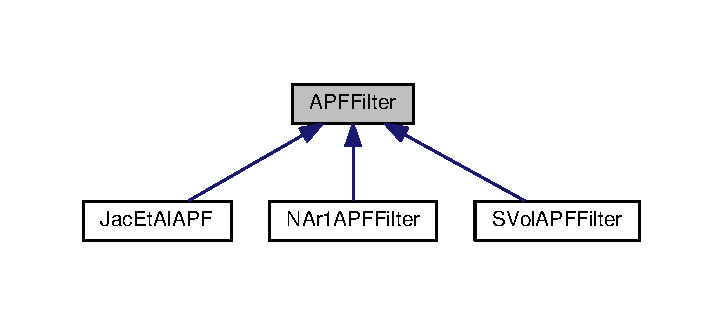
\includegraphics[width=347pt]{classAPFFilter__inherit__graph}
\end{center}
\end{figure}
\subsection*{Public Member Functions}
\begin{DoxyCompactItemize}
\item 
\hyperlink{classAPFFilter_acda2f47653ceda4bfd3d9a25d18790c7}{A\+P\+F\+Filter} (int num\+Parts, A\+P\+F\+Resamp\+Style resamp\+Technique=A\+P\+F\+Resamp\+Style\+::everytime\+\_\+multinomial, unsigned int path\+Length=0)
\begin{DoxyCompactList}\small\item\em The constructor. \end{DoxyCompactList}\item 
\hyperlink{classAPFFilter_ac2f814288c00c8b4f149cb4887d11f92}{$\sim$\+A\+P\+F\+Filter} ()\hypertarget{classAPFFilter_ac2f814288c00c8b4f149cb4887d11f92}{}\label{classAPFFilter_ac2f814288c00c8b4f149cb4887d11f92}

\begin{DoxyCompactList}\small\item\em The destructor. \end{DoxyCompactList}\item 
double \hyperlink{classAPFFilter_af9a5210f2927616dd6c82705d203b012}{get\+Log\+Cond\+Like} () const 
\begin{DoxyCompactList}\small\item\em Get the latest log conditional likelihood. \end{DoxyCompactList}\item 
const std\+::vector$<$ std\+::vector$<$ Vec $>$ $>$ \& \hyperlink{classAPFFilter_aa2ec5f04285cd1821f21ee85dcf50e3f}{get\+Full\+Parts} () const 
\begin{DoxyCompactList}\small\item\em Get the full set of particle paths. Only works if path\+Length $>$ 0 in constructor. \end{DoxyCompactList}\item 
const std\+::vector$<$ Mat $>$ \& \hyperlink{classAPFFilter_a84281845b2986f246fc132d13fd33e3d}{get\+Expectations} () const 
\begin{DoxyCompactList}\small\item\em return all stored expectations (taken with respect to \$p(x\+\_\+t$\vert$y\+\_\+\{1\+:t\})\$ \end{DoxyCompactList}\item 
const std\+::vector$<$ double $>$ \& \hyperlink{classAPFFilter_a5e552b59cc1e2adc56b06ea7925df51f}{get\+Weights} () const 
\begin{DoxyCompactList}\small\item\em Get the latest log un-\/normalized weights. \end{DoxyCompactList}\item 
void \hyperlink{classAPFFilter_adc7ee7fed78dd93309784378523e0399}{filter\+Or\+Smooth} (const Vec \&dataconst, const std\+::vector$<$ std\+::function$<$ const Mat(const Vec \&)$>$ $>$ \&fs=std\+::vector$<$ std\+::function$<$ const Mat(const Vec \&)$>$ $>$())
\begin{DoxyCompactList}\small\item\em Use a new datapoint to update the filtering distribution (or smoothing if path\+Length $>$ 0). \end{DoxyCompactList}\item 
virtual double \hyperlink{classAPFFilter_af3d1501c147477ce1128b221f7b608fd}{log\+Mu\+Ev} (const Vec \&x1)=0
\begin{DoxyCompactList}\small\item\em Evaluates the log of mu. \end{DoxyCompactList}\item 
virtual Vec \hyperlink{classAPFFilter_a2c136104f4d96e6481406ef1397ead51}{prop\+Mu} (const Vec \&xtm1)=0
\begin{DoxyCompactList}\small\item\em Evaluates the proposal distribution taking a Vec from the previous time\textquotesingle{}s state, and returning a state for the current time. \end{DoxyCompactList}\item 
virtual Vec \hyperlink{classAPFFilter_a017be49a493263156ae60ccc424f7daa}{q1\+Samp} (const Vec \&y1)=0
\begin{DoxyCompactList}\small\item\em Samples from q1. \end{DoxyCompactList}\item 
virtual Vec \hyperlink{classAPFFilter_a367c77209129a84f3d64ff3bcaaac513}{f\+Samp} (const Vec \&xtm1)=0
\begin{DoxyCompactList}\small\item\em Samples from f. \end{DoxyCompactList}\item 
virtual double \hyperlink{classAPFFilter_a18ba363183c0c92e6c58d6f3faccbea7}{log\+Q1\+Ev} (const Vec \&x1, const Vec \&y1)=0
\begin{DoxyCompactList}\small\item\em Evaluates the log of q1. \end{DoxyCompactList}\item 
virtual double \hyperlink{classAPFFilter_ac2d0b5329d7ae123ae4de5dddefb5591}{log\+G\+Ev} (const Vec \&yt, const Vec \&xt)=0
\begin{DoxyCompactList}\small\item\em Evaluates the log of g. \end{DoxyCompactList}\end{DoxyCompactItemize}


\subsection{Detailed Description}
A base-\/class for Auxiliary Particle Filtering. 

\begin{DoxyAuthor}{Author}
taylor 
\end{DoxyAuthor}
\begin{DoxyDate}{Date}
09/09/17 
\end{DoxyDate}


\subsection{Constructor \& Destructor Documentation}
\index{A\+P\+F\+Filter@{A\+P\+F\+Filter}!A\+P\+F\+Filter@{A\+P\+F\+Filter}}
\index{A\+P\+F\+Filter@{A\+P\+F\+Filter}!A\+P\+F\+Filter@{A\+P\+F\+Filter}}
\subsubsection[{\texorpdfstring{A\+P\+F\+Filter(int num\+Parts, A\+P\+F\+Resamp\+Style resamp\+Technique=\+A\+P\+F\+Resamp\+Style\+::everytime\+\_\+multinomial, unsigned int path\+Length=0)}{APFFilter(int numParts, APFResampStyle resampTechnique=APFResampStyle::everytime_multinomial, unsigned int pathLength=0)}}]{\setlength{\rightskip}{0pt plus 5cm}A\+P\+F\+Filter\+::\+A\+P\+F\+Filter (
\begin{DoxyParamCaption}
\item[{int}]{num\+Parts, }
\item[{A\+P\+F\+Resamp\+Style}]{resamp\+Technique = {\ttfamily APFResampStyle\+:\+:everytime\+\_\+multinomial}, }
\item[{unsigned int}]{path\+Length = {\ttfamily 0}}
\end{DoxyParamCaption}
)}\hypertarget{classAPFFilter_acda2f47653ceda4bfd3d9a25d18790c7}{}\label{classAPFFilter_acda2f47653ceda4bfd3d9a25d18790c7}


The constructor. 


\begin{DoxyParams}{Parameters}
{\em num\+Parts} & the number of particles you want to use. \\
\hline
{\em resamp\+Technique} & the resampling style. \\
\hline
{\em path\+Length} & set to 0 if you are filtering. Otherwise, if you wish to retain samples of the entire path, set to time length of data. \\
\hline
\end{DoxyParams}


\subsection{Member Function Documentation}
\index{A\+P\+F\+Filter@{A\+P\+F\+Filter}!filter\+Or\+Smooth@{filter\+Or\+Smooth}}
\index{filter\+Or\+Smooth@{filter\+Or\+Smooth}!A\+P\+F\+Filter@{A\+P\+F\+Filter}}
\subsubsection[{\texorpdfstring{filter\+Or\+Smooth(const Vec \&dataconst, const std\+::vector$<$ std\+::function$<$ const Mat(const Vec \&)$>$ $>$ \&fs=std\+::vector$<$ std\+::function$<$ const Mat(const Vec \&)$>$ $>$())}{filterOrSmooth(const Vec &dataconst, const std::vector< std::function< const Mat(const Vec &)> > &fs=std::vector< std::function< const Mat(const Vec &)> >())}}]{\setlength{\rightskip}{0pt plus 5cm}void A\+P\+F\+Filter\+::filter\+Or\+Smooth (
\begin{DoxyParamCaption}
\item[{const Vec \&}]{dataconst, }
\item[{const std\+::vector$<$ std\+::function$<$ const Mat(const Vec \&)$>$ $>$ \&}]{fs = {\ttfamily std\+:\+:vector$<$~std\+:\+:function$<$~const~Mat(const~Vec~\&)$>$~$>$()}}
\end{DoxyParamCaption}
)}\hypertarget{classAPFFilter_adc7ee7fed78dd93309784378523e0399}{}\label{classAPFFilter_adc7ee7fed78dd93309784378523e0399}


Use a new datapoint to update the filtering distribution (or smoothing if path\+Length $>$ 0). 


\begin{DoxyParams}{Parameters}
{\em a} & Vec representing the data \\
\hline
{\em a} & std\+::vector of callback functions that are used to calculate expectations with respect to the filtering distribution. \\
\hline
\end{DoxyParams}
\index{A\+P\+F\+Filter@{A\+P\+F\+Filter}!f\+Samp@{f\+Samp}}
\index{f\+Samp@{f\+Samp}!A\+P\+F\+Filter@{A\+P\+F\+Filter}}
\subsubsection[{\texorpdfstring{f\+Samp(const Vec \&xtm1)=0}{fSamp(const Vec &xtm1)=0}}]{\setlength{\rightskip}{0pt plus 5cm}virtual Vec A\+P\+F\+Filter\+::f\+Samp (
\begin{DoxyParamCaption}
\item[{const Vec \&}]{xtm1}
\end{DoxyParamCaption}
)\hspace{0.3cm}{\ttfamily [pure virtual]}}\hypertarget{classAPFFilter_a367c77209129a84f3d64ff3bcaaac513}{}\label{classAPFFilter_a367c77209129a84f3d64ff3bcaaac513}


Samples from f. 


\begin{DoxyParams}{Parameters}
{\em xtm1} & a Vec representing the previous time\textquotesingle{}s state. \\
\hline
\end{DoxyParams}
\begin{DoxyReturn}{Returns}
a Vec state sample for the current time. 
\end{DoxyReturn}


Implemented in \hyperlink{classJacEtAlAPF_abb98b3c8dcb28b43bebf54c15e0f8616}{Jac\+Et\+Al\+A\+PF}, \hyperlink{classSVolAPFFilter_a3e24042d1c2763c80fe56ab9a5359aac}{S\+Vol\+A\+P\+F\+Filter}, and \hyperlink{classNAr1APFFilter_a7490ba7d06d2d82930afce64100cce99}{N\+Ar1\+A\+P\+F\+Filter}.

\index{A\+P\+F\+Filter@{A\+P\+F\+Filter}!get\+Expectations@{get\+Expectations}}
\index{get\+Expectations@{get\+Expectations}!A\+P\+F\+Filter@{A\+P\+F\+Filter}}
\subsubsection[{\texorpdfstring{get\+Expectations() const }{getExpectations() const }}]{\setlength{\rightskip}{0pt plus 5cm}const std\+::vector$<$Mat$>$\& A\+P\+F\+Filter\+::get\+Expectations (
\begin{DoxyParamCaption}
{}
\end{DoxyParamCaption}
) const}\hypertarget{classAPFFilter_a84281845b2986f246fc132d13fd33e3d}{}\label{classAPFFilter_a84281845b2986f246fc132d13fd33e3d}


return all stored expectations (taken with respect to \$p(x\+\_\+t$\vert$y\+\_\+\{1\+:t\})\$ 

\begin{DoxyReturn}{Returns}
return a std\+::vector$<$\+Mat$>$ of expectations. How many depends on how many callbacks you gave to 
\end{DoxyReturn}
\index{A\+P\+F\+Filter@{A\+P\+F\+Filter}!get\+Full\+Parts@{get\+Full\+Parts}}
\index{get\+Full\+Parts@{get\+Full\+Parts}!A\+P\+F\+Filter@{A\+P\+F\+Filter}}
\subsubsection[{\texorpdfstring{get\+Full\+Parts() const }{getFullParts() const }}]{\setlength{\rightskip}{0pt plus 5cm}const std\+::vector$<$std\+::vector$<$Vec$>$ $>$\& A\+P\+F\+Filter\+::get\+Full\+Parts (
\begin{DoxyParamCaption}
{}
\end{DoxyParamCaption}
) const}\hypertarget{classAPFFilter_aa2ec5f04285cd1821f21ee85dcf50e3f}{}\label{classAPFFilter_aa2ec5f04285cd1821f21ee85dcf50e3f}


Get the full set of particle paths. Only works if path\+Length $>$ 0 in constructor. 

\begin{DoxyReturn}{Returns}
The full set of particle paths as std\+::vector$<$std\+::vector$<$\+Vec$>$ $>$. 
\end{DoxyReturn}
\index{A\+P\+F\+Filter@{A\+P\+F\+Filter}!get\+Log\+Cond\+Like@{get\+Log\+Cond\+Like}}
\index{get\+Log\+Cond\+Like@{get\+Log\+Cond\+Like}!A\+P\+F\+Filter@{A\+P\+F\+Filter}}
\subsubsection[{\texorpdfstring{get\+Log\+Cond\+Like() const }{getLogCondLike() const }}]{\setlength{\rightskip}{0pt plus 5cm}double A\+P\+F\+Filter\+::get\+Log\+Cond\+Like (
\begin{DoxyParamCaption}
{}
\end{DoxyParamCaption}
) const}\hypertarget{classAPFFilter_af9a5210f2927616dd6c82705d203b012}{}\label{classAPFFilter_af9a5210f2927616dd6c82705d203b012}


Get the latest log conditional likelihood. 

\begin{DoxyReturn}{Returns}
a double of the most recent conditional likelihood. 
\end{DoxyReturn}
\index{A\+P\+F\+Filter@{A\+P\+F\+Filter}!get\+Weights@{get\+Weights}}
\index{get\+Weights@{get\+Weights}!A\+P\+F\+Filter@{A\+P\+F\+Filter}}
\subsubsection[{\texorpdfstring{get\+Weights() const }{getWeights() const }}]{\setlength{\rightskip}{0pt plus 5cm}const std\+::vector$<$double$>$\& A\+P\+F\+Filter\+::get\+Weights (
\begin{DoxyParamCaption}
{}
\end{DoxyParamCaption}
) const}\hypertarget{classAPFFilter_a5e552b59cc1e2adc56b06ea7925df51f}{}\label{classAPFFilter_a5e552b59cc1e2adc56b06ea7925df51f}


Get the latest log un-\/normalized weights. 

\begin{DoxyReturn}{Returns}
a std\+::vector$<$double$>$ of the log un norm weights. 
\end{DoxyReturn}
\index{A\+P\+F\+Filter@{A\+P\+F\+Filter}!log\+G\+Ev@{log\+G\+Ev}}
\index{log\+G\+Ev@{log\+G\+Ev}!A\+P\+F\+Filter@{A\+P\+F\+Filter}}
\subsubsection[{\texorpdfstring{log\+G\+Ev(const Vec \&yt, const Vec \&xt)=0}{logGEv(const Vec &yt, const Vec &xt)=0}}]{\setlength{\rightskip}{0pt plus 5cm}virtual double A\+P\+F\+Filter\+::log\+G\+Ev (
\begin{DoxyParamCaption}
\item[{const Vec \&}]{yt, }
\item[{const Vec \&}]{xt}
\end{DoxyParamCaption}
)\hspace{0.3cm}{\ttfamily [pure virtual]}}\hypertarget{classAPFFilter_ac2d0b5329d7ae123ae4de5dddefb5591}{}\label{classAPFFilter_ac2d0b5329d7ae123ae4de5dddefb5591}


Evaluates the log of g. 


\begin{DoxyParams}{Parameters}
{\em yt} & a Vec representing time t\textquotesingle{}s data observation. \\
\hline
{\em xt} & a Vec representing time t\textquotesingle{}s state. \\
\hline
\end{DoxyParams}
\begin{DoxyReturn}{Returns}
a double evaluation. 
\end{DoxyReturn}


Implemented in \hyperlink{classJacEtAlAPF_a0cd22a37063906eddf47f8b4887919eb}{Jac\+Et\+Al\+A\+PF}, \hyperlink{classNAr1APFFilter_afabcd7acb729a62955856c9737e76059}{N\+Ar1\+A\+P\+F\+Filter}, and \hyperlink{classSVolAPFFilter_ac0b9ba8b7fcb918c011bb662f3306d19}{S\+Vol\+A\+P\+F\+Filter}.

\index{A\+P\+F\+Filter@{A\+P\+F\+Filter}!log\+Mu\+Ev@{log\+Mu\+Ev}}
\index{log\+Mu\+Ev@{log\+Mu\+Ev}!A\+P\+F\+Filter@{A\+P\+F\+Filter}}
\subsubsection[{\texorpdfstring{log\+Mu\+Ev(const Vec \&x1)=0}{logMuEv(const Vec &x1)=0}}]{\setlength{\rightskip}{0pt plus 5cm}virtual double A\+P\+F\+Filter\+::log\+Mu\+Ev (
\begin{DoxyParamCaption}
\item[{const Vec \&}]{x1}
\end{DoxyParamCaption}
)\hspace{0.3cm}{\ttfamily [pure virtual]}}\hypertarget{classAPFFilter_af3d1501c147477ce1128b221f7b608fd}{}\label{classAPFFilter_af3d1501c147477ce1128b221f7b608fd}


Evaluates the log of mu. 


\begin{DoxyParams}{Parameters}
{\em x1} & a Vec representing time 1\textquotesingle{}s state. \\
\hline
\end{DoxyParams}
\begin{DoxyReturn}{Returns}
a double evaluation. 
\end{DoxyReturn}


Implemented in \hyperlink{classJacEtAlAPF_ac61d6bcb7a63bc95fda6e138255c2535}{Jac\+Et\+Al\+A\+PF}, \hyperlink{classNAr1APFFilter_ad85b9a81c93f86ebcc8e837bb2ca010f}{N\+Ar1\+A\+P\+F\+Filter}, and \hyperlink{classSVolAPFFilter_ac019751d65847aabfb4a5b4cdcfbcf4c}{S\+Vol\+A\+P\+F\+Filter}.

\index{A\+P\+F\+Filter@{A\+P\+F\+Filter}!log\+Q1\+Ev@{log\+Q1\+Ev}}
\index{log\+Q1\+Ev@{log\+Q1\+Ev}!A\+P\+F\+Filter@{A\+P\+F\+Filter}}
\subsubsection[{\texorpdfstring{log\+Q1\+Ev(const Vec \&x1, const Vec \&y1)=0}{logQ1Ev(const Vec &x1, const Vec &y1)=0}}]{\setlength{\rightskip}{0pt plus 5cm}virtual double A\+P\+F\+Filter\+::log\+Q1\+Ev (
\begin{DoxyParamCaption}
\item[{const Vec \&}]{x1, }
\item[{const Vec \&}]{y1}
\end{DoxyParamCaption}
)\hspace{0.3cm}{\ttfamily [pure virtual]}}\hypertarget{classAPFFilter_a18ba363183c0c92e6c58d6f3faccbea7}{}\label{classAPFFilter_a18ba363183c0c92e6c58d6f3faccbea7}


Evaluates the log of q1. 


\begin{DoxyParams}{Parameters}
{\em x1} & a Vec representing time 1\textquotesingle{}s state. \\
\hline
{\em y1} & a Vec representing time 1\textquotesingle{}s data observation. \\
\hline
\end{DoxyParams}
\begin{DoxyReturn}{Returns}
a double evaluation. 
\end{DoxyReturn}


Implemented in \hyperlink{classJacEtAlAPF_a36e56af90cafe323fc42d8eaf75402f9}{Jac\+Et\+Al\+A\+PF}, \hyperlink{classNAr1APFFilter_a0839d99fe62312b8a2c5c781b879fa79}{N\+Ar1\+A\+P\+F\+Filter}, and \hyperlink{classSVolAPFFilter_ade59e30d3d1517a0c64fc44bc027d53c}{S\+Vol\+A\+P\+F\+Filter}.

\index{A\+P\+F\+Filter@{A\+P\+F\+Filter}!prop\+Mu@{prop\+Mu}}
\index{prop\+Mu@{prop\+Mu}!A\+P\+F\+Filter@{A\+P\+F\+Filter}}
\subsubsection[{\texorpdfstring{prop\+Mu(const Vec \&xtm1)=0}{propMu(const Vec &xtm1)=0}}]{\setlength{\rightskip}{0pt plus 5cm}virtual Vec A\+P\+F\+Filter\+::prop\+Mu (
\begin{DoxyParamCaption}
\item[{const Vec \&}]{xtm1}
\end{DoxyParamCaption}
)\hspace{0.3cm}{\ttfamily [pure virtual]}}\hypertarget{classAPFFilter_a2c136104f4d96e6481406ef1397ead51}{}\label{classAPFFilter_a2c136104f4d96e6481406ef1397ead51}


Evaluates the proposal distribution taking a Vec from the previous time\textquotesingle{}s state, and returning a state for the current time. 


\begin{DoxyParams}{Parameters}
{\em xtm1} & a Vec representing the previous time\textquotesingle{}s state. \\
\hline
\end{DoxyParams}
\begin{DoxyReturn}{Returns}
a Vec representing a likely current time state, to be used by the observation density. 
\end{DoxyReturn}


Implemented in \hyperlink{classJacEtAlAPF_a3066fe2bd0b399a85eaf51ecdb1c3660}{Jac\+Et\+Al\+A\+PF}, \hyperlink{classNAr1APFFilter_a92a000138b5440613ab85c3811eb5525}{N\+Ar1\+A\+P\+F\+Filter}, and \hyperlink{classSVolAPFFilter_a5a5d8ac387f71cb64d8da66c38bbff71}{S\+Vol\+A\+P\+F\+Filter}.

\index{A\+P\+F\+Filter@{A\+P\+F\+Filter}!q1\+Samp@{q1\+Samp}}
\index{q1\+Samp@{q1\+Samp}!A\+P\+F\+Filter@{A\+P\+F\+Filter}}
\subsubsection[{\texorpdfstring{q1\+Samp(const Vec \&y1)=0}{q1Samp(const Vec &y1)=0}}]{\setlength{\rightskip}{0pt plus 5cm}virtual Vec A\+P\+F\+Filter\+::q1\+Samp (
\begin{DoxyParamCaption}
\item[{const Vec \&}]{y1}
\end{DoxyParamCaption}
)\hspace{0.3cm}{\ttfamily [pure virtual]}}\hypertarget{classAPFFilter_a017be49a493263156ae60ccc424f7daa}{}\label{classAPFFilter_a017be49a493263156ae60ccc424f7daa}


Samples from q1. 


\begin{DoxyParams}{Parameters}
{\em y1} & a Vec representing time 1\textquotesingle{}s data point. \\
\hline
\end{DoxyParams}
\begin{DoxyReturn}{Returns}
a Vec sample for time 1\textquotesingle{}s state. 
\end{DoxyReturn}


Implemented in \hyperlink{classJacEtAlAPF_afdd084c634e7ad591499a6c8c90ee9d0}{Jac\+Et\+Al\+A\+PF}, \hyperlink{classNAr1APFFilter_a294a2044c95ba6e013758fa62f3ef979}{N\+Ar1\+A\+P\+F\+Filter}, and \hyperlink{classSVolAPFFilter_a9da55ac2cfbc51ce0bc65a335942b1b6}{S\+Vol\+A\+P\+F\+Filter}.



The documentation for this class was generated from the following file\+:\begin{DoxyCompactItemize}
\item 
include/apf\+\_\+filter.\+h\end{DoxyCompactItemize}

\hypertarget{classAPFSmoother}{}\section{A\+P\+F\+Smoother Class Reference}
\label{classAPFSmoother}\index{A\+P\+F\+Smoother@{A\+P\+F\+Smoother}}


A base-\/class for Auxiliary Particle Filtering. Particle smoothing only; no filtering.  




{\ttfamily \#include $<$apf\+\_\+smooth.\+h$>$}

\subsection*{Public Member Functions}
\begin{DoxyCompactItemize}
\item 
\hyperlink{classAPFSmoother_a51d9a70bc16259592f9a92fcd1008bc3}{A\+P\+F\+Smoother} (int num\+Parts, unsigned int path\+Length, \hyperlink{apf__filter_8h_a187a7338bc8872e7607cf1ea4ffed47b}{A\+P\+F\+Resamp\+Style} resamp\+Technique=A\+P\+F\+Resamp\+Style\+::everytime\+\_\+multinomial)
\begin{DoxyCompactList}\small\item\em The constructor. \end{DoxyCompactList}\item 
\hyperlink{classAPFSmoother_a12ee69daa15fc1f59a8efd9303894896}{$\sim$\+A\+P\+F\+Smoother} ()\hypertarget{classAPFSmoother_a12ee69daa15fc1f59a8efd9303894896}{}\label{classAPFSmoother_a12ee69daa15fc1f59a8efd9303894896}

\begin{DoxyCompactList}\small\item\em The destructor. \end{DoxyCompactList}\item 
double \hyperlink{classAPFSmoother_af78387b6b79bb2d3c3b44663e7fc31f3}{get\+Log\+Cond\+Like} () const 
\begin{DoxyCompactList}\small\item\em Get the latest log conditional likelihood. \end{DoxyCompactList}\item 
std\+::vector$<$ std\+::vector$<$ \hyperlink{apf__filter_8h_a4c7df05c6f5e8a0d15ae14bcdbc07152}{Vec} $>$ $>$ \hyperlink{classAPFSmoother_af9bd42db37a53bc03f238a6db829102c}{get\+Full\+Parts} () const 
\begin{DoxyCompactList}\small\item\em Get the full set of particle paths. Only works if path\+Length $>$ 0 in constructor. \end{DoxyCompactList}\item 
std\+::vector$<$ double $>$ \hyperlink{classAPFSmoother_a6bc97edb04f65e1f038f753b9fb2dd9c}{get\+Weights} () const 
\begin{DoxyCompactList}\small\item\em Get the latest log un-\/normalized weights. \end{DoxyCompactList}\item 
void \hyperlink{classAPFSmoother_acaf872bc7356e60198fedce0665afeb6}{smooth} (const \hyperlink{apf__filter_8h_a4c7df05c6f5e8a0d15ae14bcdbc07152}{Vec} \&data)
\begin{DoxyCompactList}\small\item\em Use a new datapoint to update the smoothing distribution. \end{DoxyCompactList}\item 
virtual double \hyperlink{classAPFSmoother_a6afc79350b182fe4083936d1abd2beda}{log\+Mu\+Ev} (const \hyperlink{apf__filter_8h_a4c7df05c6f5e8a0d15ae14bcdbc07152}{Vec} \&x1)=0
\begin{DoxyCompactList}\small\item\em Evaluates the log of mu. \end{DoxyCompactList}\item 
virtual \hyperlink{apf__filter_8h_a4c7df05c6f5e8a0d15ae14bcdbc07152}{Vec} \hyperlink{classAPFSmoother_a8c95c24e4e6f5699ef6f9b95c64fc9eb}{prop\+Mu} (const \hyperlink{apf__filter_8h_a4c7df05c6f5e8a0d15ae14bcdbc07152}{Vec} \&xtm1)=0
\begin{DoxyCompactList}\small\item\em Evaluates the proposal distribution taking a Vec from the previous time\textquotesingle{}s state, and returning a state for the current time. \end{DoxyCompactList}\item 
virtual \hyperlink{apf__filter_8h_a4c7df05c6f5e8a0d15ae14bcdbc07152}{Vec} \hyperlink{classAPFSmoother_ae1b444849e0e2882c00e928409d8fc4b}{q1\+Samp} (const \hyperlink{apf__filter_8h_a4c7df05c6f5e8a0d15ae14bcdbc07152}{Vec} \&y1)=0
\begin{DoxyCompactList}\small\item\em Samples from q1. \end{DoxyCompactList}\item 
virtual \hyperlink{apf__filter_8h_a4c7df05c6f5e8a0d15ae14bcdbc07152}{Vec} \hyperlink{classAPFSmoother_a823b3f5d1d942f5305d05dfd318f4851}{f\+Samp} (const \hyperlink{apf__filter_8h_a4c7df05c6f5e8a0d15ae14bcdbc07152}{Vec} \&xtm1)=0
\begin{DoxyCompactList}\small\item\em Samples from f. \end{DoxyCompactList}\item 
virtual double \hyperlink{classAPFSmoother_a4353091a34dac9dd072f407a593aea03}{log\+Q1\+Ev} (const \hyperlink{apf__filter_8h_a4c7df05c6f5e8a0d15ae14bcdbc07152}{Vec} \&x1, const \hyperlink{apf__filter_8h_a4c7df05c6f5e8a0d15ae14bcdbc07152}{Vec} \&y1)=0
\begin{DoxyCompactList}\small\item\em Evaluates the log of q1. \end{DoxyCompactList}\item 
virtual double \hyperlink{classAPFSmoother_acd249cf906d89162f367ded9f02c7793}{log\+G\+Ev} (const \hyperlink{apf__filter_8h_a4c7df05c6f5e8a0d15ae14bcdbc07152}{Vec} \&yt, const \hyperlink{apf__filter_8h_a4c7df05c6f5e8a0d15ae14bcdbc07152}{Vec} \&xt)=0
\begin{DoxyCompactList}\small\item\em Evaluates the log of g. \end{DoxyCompactList}\end{DoxyCompactItemize}


\subsection{Detailed Description}
A base-\/class for Auxiliary Particle Filtering. Particle smoothing only; no filtering. 

\begin{DoxyAuthor}{Author}
taylor 
\end{DoxyAuthor}
\begin{DoxyDate}{Date}
09/09/17 
\end{DoxyDate}


\subsection{Constructor \& Destructor Documentation}
\index{A\+P\+F\+Smoother@{A\+P\+F\+Smoother}!A\+P\+F\+Smoother@{A\+P\+F\+Smoother}}
\index{A\+P\+F\+Smoother@{A\+P\+F\+Smoother}!A\+P\+F\+Smoother@{A\+P\+F\+Smoother}}
\subsubsection[{\texorpdfstring{A\+P\+F\+Smoother(int num\+Parts, unsigned int path\+Length, A\+P\+F\+Resamp\+Style resamp\+Technique=\+A\+P\+F\+Resamp\+Style\+::everytime\+\_\+multinomial)}{APFSmoother(int numParts, unsigned int pathLength, APFResampStyle resampTechnique=APFResampStyle::everytime_multinomial)}}]{\setlength{\rightskip}{0pt plus 5cm}A\+P\+F\+Smoother\+::\+A\+P\+F\+Smoother (
\begin{DoxyParamCaption}
\item[{int}]{num\+Parts, }
\item[{unsigned int}]{path\+Length, }
\item[{{\bf A\+P\+F\+Resamp\+Style}}]{resamp\+Technique = {\ttfamily APFResampStyle\+:\+:everytime\+\_\+multinomial}}
\end{DoxyParamCaption}
)}\hypertarget{classAPFSmoother_a51d9a70bc16259592f9a92fcd1008bc3}{}\label{classAPFSmoother_a51d9a70bc16259592f9a92fcd1008bc3}


The constructor. 


\begin{DoxyParams}{Parameters}
{\em num\+Parts} & the number of particles you want to use. \\
\hline
{\em resamp\+Technique} & the resampling style. \\
\hline
{\em path\+Length} & set to 0 if you are filtering. Otherwise, if you wish to retain samples of the entire path, set to time length of data. \\
\hline
\end{DoxyParams}


\subsection{Member Function Documentation}
\index{A\+P\+F\+Smoother@{A\+P\+F\+Smoother}!f\+Samp@{f\+Samp}}
\index{f\+Samp@{f\+Samp}!A\+P\+F\+Smoother@{A\+P\+F\+Smoother}}
\subsubsection[{\texorpdfstring{f\+Samp(const Vec \&xtm1)=0}{fSamp(const Vec &xtm1)=0}}]{\setlength{\rightskip}{0pt plus 5cm}virtual {\bf Vec} A\+P\+F\+Smoother\+::f\+Samp (
\begin{DoxyParamCaption}
\item[{const {\bf Vec} \&}]{xtm1}
\end{DoxyParamCaption}
)\hspace{0.3cm}{\ttfamily [pure virtual]}}\hypertarget{classAPFSmoother_a823b3f5d1d942f5305d05dfd318f4851}{}\label{classAPFSmoother_a823b3f5d1d942f5305d05dfd318f4851}


Samples from f. 


\begin{DoxyParams}{Parameters}
{\em xtm1} & a Vec representing the previous time\textquotesingle{}s state. \\
\hline
\end{DoxyParams}
\begin{DoxyReturn}{Returns}
a Vec state sample for the current time. 
\end{DoxyReturn}
\index{A\+P\+F\+Smoother@{A\+P\+F\+Smoother}!get\+Full\+Parts@{get\+Full\+Parts}}
\index{get\+Full\+Parts@{get\+Full\+Parts}!A\+P\+F\+Smoother@{A\+P\+F\+Smoother}}
\subsubsection[{\texorpdfstring{get\+Full\+Parts() const }{getFullParts() const }}]{\setlength{\rightskip}{0pt plus 5cm}std\+::vector$<$std\+::vector$<${\bf Vec}$>$ $>$ A\+P\+F\+Smoother\+::get\+Full\+Parts (
\begin{DoxyParamCaption}
{}
\end{DoxyParamCaption}
) const}\hypertarget{classAPFSmoother_af9bd42db37a53bc03f238a6db829102c}{}\label{classAPFSmoother_af9bd42db37a53bc03f238a6db829102c}


Get the full set of particle paths. Only works if path\+Length $>$ 0 in constructor. 

\begin{DoxyReturn}{Returns}
The full set of particle paths as std\+::vector$<$std\+::vector$<$\+Vec$>$ $>$. 
\end{DoxyReturn}
\index{A\+P\+F\+Smoother@{A\+P\+F\+Smoother}!get\+Log\+Cond\+Like@{get\+Log\+Cond\+Like}}
\index{get\+Log\+Cond\+Like@{get\+Log\+Cond\+Like}!A\+P\+F\+Smoother@{A\+P\+F\+Smoother}}
\subsubsection[{\texorpdfstring{get\+Log\+Cond\+Like() const }{getLogCondLike() const }}]{\setlength{\rightskip}{0pt plus 5cm}double A\+P\+F\+Smoother\+::get\+Log\+Cond\+Like (
\begin{DoxyParamCaption}
{}
\end{DoxyParamCaption}
) const}\hypertarget{classAPFSmoother_af78387b6b79bb2d3c3b44663e7fc31f3}{}\label{classAPFSmoother_af78387b6b79bb2d3c3b44663e7fc31f3}


Get the latest log conditional likelihood. 

\begin{DoxyReturn}{Returns}
a double of the most recent conditional likelihood. 
\end{DoxyReturn}
\index{A\+P\+F\+Smoother@{A\+P\+F\+Smoother}!get\+Weights@{get\+Weights}}
\index{get\+Weights@{get\+Weights}!A\+P\+F\+Smoother@{A\+P\+F\+Smoother}}
\subsubsection[{\texorpdfstring{get\+Weights() const }{getWeights() const }}]{\setlength{\rightskip}{0pt plus 5cm}std\+::vector$<$double$>$ A\+P\+F\+Smoother\+::get\+Weights (
\begin{DoxyParamCaption}
{}
\end{DoxyParamCaption}
) const}\hypertarget{classAPFSmoother_a6bc97edb04f65e1f038f753b9fb2dd9c}{}\label{classAPFSmoother_a6bc97edb04f65e1f038f753b9fb2dd9c}


Get the latest log un-\/normalized weights. 

\begin{DoxyReturn}{Returns}
a std\+::vector$<$double$>$ of the log un norm weights. 
\end{DoxyReturn}
\index{A\+P\+F\+Smoother@{A\+P\+F\+Smoother}!log\+G\+Ev@{log\+G\+Ev}}
\index{log\+G\+Ev@{log\+G\+Ev}!A\+P\+F\+Smoother@{A\+P\+F\+Smoother}}
\subsubsection[{\texorpdfstring{log\+G\+Ev(const Vec \&yt, const Vec \&xt)=0}{logGEv(const Vec &yt, const Vec &xt)=0}}]{\setlength{\rightskip}{0pt plus 5cm}virtual double A\+P\+F\+Smoother\+::log\+G\+Ev (
\begin{DoxyParamCaption}
\item[{const {\bf Vec} \&}]{yt, }
\item[{const {\bf Vec} \&}]{xt}
\end{DoxyParamCaption}
)\hspace{0.3cm}{\ttfamily [pure virtual]}}\hypertarget{classAPFSmoother_acd249cf906d89162f367ded9f02c7793}{}\label{classAPFSmoother_acd249cf906d89162f367ded9f02c7793}


Evaluates the log of g. 


\begin{DoxyParams}{Parameters}
{\em yt} & a Vec representing time t\textquotesingle{}s data observation. \\
\hline
{\em xt} & a Vec representing time t\textquotesingle{}s state. \\
\hline
\end{DoxyParams}
\begin{DoxyReturn}{Returns}
a double evaluation. 
\end{DoxyReturn}
\index{A\+P\+F\+Smoother@{A\+P\+F\+Smoother}!log\+Mu\+Ev@{log\+Mu\+Ev}}
\index{log\+Mu\+Ev@{log\+Mu\+Ev}!A\+P\+F\+Smoother@{A\+P\+F\+Smoother}}
\subsubsection[{\texorpdfstring{log\+Mu\+Ev(const Vec \&x1)=0}{logMuEv(const Vec &x1)=0}}]{\setlength{\rightskip}{0pt plus 5cm}virtual double A\+P\+F\+Smoother\+::log\+Mu\+Ev (
\begin{DoxyParamCaption}
\item[{const {\bf Vec} \&}]{x1}
\end{DoxyParamCaption}
)\hspace{0.3cm}{\ttfamily [pure virtual]}}\hypertarget{classAPFSmoother_a6afc79350b182fe4083936d1abd2beda}{}\label{classAPFSmoother_a6afc79350b182fe4083936d1abd2beda}


Evaluates the log of mu. 


\begin{DoxyParams}{Parameters}
{\em x1} & a Vec representing time 1\textquotesingle{}s state. \\
\hline
\end{DoxyParams}
\begin{DoxyReturn}{Returns}
a double evaluation. 
\end{DoxyReturn}
\index{A\+P\+F\+Smoother@{A\+P\+F\+Smoother}!log\+Q1\+Ev@{log\+Q1\+Ev}}
\index{log\+Q1\+Ev@{log\+Q1\+Ev}!A\+P\+F\+Smoother@{A\+P\+F\+Smoother}}
\subsubsection[{\texorpdfstring{log\+Q1\+Ev(const Vec \&x1, const Vec \&y1)=0}{logQ1Ev(const Vec &x1, const Vec &y1)=0}}]{\setlength{\rightskip}{0pt plus 5cm}virtual double A\+P\+F\+Smoother\+::log\+Q1\+Ev (
\begin{DoxyParamCaption}
\item[{const {\bf Vec} \&}]{x1, }
\item[{const {\bf Vec} \&}]{y1}
\end{DoxyParamCaption}
)\hspace{0.3cm}{\ttfamily [pure virtual]}}\hypertarget{classAPFSmoother_a4353091a34dac9dd072f407a593aea03}{}\label{classAPFSmoother_a4353091a34dac9dd072f407a593aea03}


Evaluates the log of q1. 


\begin{DoxyParams}{Parameters}
{\em x1} & a Vec representing time 1\textquotesingle{}s state. \\
\hline
{\em y1} & a Vec representing time 1\textquotesingle{}s data observation. \\
\hline
\end{DoxyParams}
\begin{DoxyReturn}{Returns}
a double evaluation. 
\end{DoxyReturn}
\index{A\+P\+F\+Smoother@{A\+P\+F\+Smoother}!prop\+Mu@{prop\+Mu}}
\index{prop\+Mu@{prop\+Mu}!A\+P\+F\+Smoother@{A\+P\+F\+Smoother}}
\subsubsection[{\texorpdfstring{prop\+Mu(const Vec \&xtm1)=0}{propMu(const Vec &xtm1)=0}}]{\setlength{\rightskip}{0pt plus 5cm}virtual {\bf Vec} A\+P\+F\+Smoother\+::prop\+Mu (
\begin{DoxyParamCaption}
\item[{const {\bf Vec} \&}]{xtm1}
\end{DoxyParamCaption}
)\hspace{0.3cm}{\ttfamily [pure virtual]}}\hypertarget{classAPFSmoother_a8c95c24e4e6f5699ef6f9b95c64fc9eb}{}\label{classAPFSmoother_a8c95c24e4e6f5699ef6f9b95c64fc9eb}


Evaluates the proposal distribution taking a Vec from the previous time\textquotesingle{}s state, and returning a state for the current time. 


\begin{DoxyParams}{Parameters}
{\em xtm1} & a Vec representing the previous time\textquotesingle{}s state. \\
\hline
\end{DoxyParams}
\begin{DoxyReturn}{Returns}
a Vec representing a likely current time state, to be used by the observation density. 
\end{DoxyReturn}
\index{A\+P\+F\+Smoother@{A\+P\+F\+Smoother}!q1\+Samp@{q1\+Samp}}
\index{q1\+Samp@{q1\+Samp}!A\+P\+F\+Smoother@{A\+P\+F\+Smoother}}
\subsubsection[{\texorpdfstring{q1\+Samp(const Vec \&y1)=0}{q1Samp(const Vec &y1)=0}}]{\setlength{\rightskip}{0pt plus 5cm}virtual {\bf Vec} A\+P\+F\+Smoother\+::q1\+Samp (
\begin{DoxyParamCaption}
\item[{const {\bf Vec} \&}]{y1}
\end{DoxyParamCaption}
)\hspace{0.3cm}{\ttfamily [pure virtual]}}\hypertarget{classAPFSmoother_ae1b444849e0e2882c00e928409d8fc4b}{}\label{classAPFSmoother_ae1b444849e0e2882c00e928409d8fc4b}


Samples from q1. 


\begin{DoxyParams}{Parameters}
{\em y1} & a Vec representing time 1\textquotesingle{}s data point. \\
\hline
\end{DoxyParams}
\begin{DoxyReturn}{Returns}
a Vec sample for time 1\textquotesingle{}s state. 
\end{DoxyReturn}
\index{A\+P\+F\+Smoother@{A\+P\+F\+Smoother}!smooth@{smooth}}
\index{smooth@{smooth}!A\+P\+F\+Smoother@{A\+P\+F\+Smoother}}
\subsubsection[{\texorpdfstring{smooth(const Vec \&data)}{smooth(const Vec &data)}}]{\setlength{\rightskip}{0pt plus 5cm}void A\+P\+F\+Smoother\+::smooth (
\begin{DoxyParamCaption}
\item[{const {\bf Vec} \&}]{data}
\end{DoxyParamCaption}
)}\hypertarget{classAPFSmoother_acaf872bc7356e60198fedce0665afeb6}{}\label{classAPFSmoother_acaf872bc7356e60198fedce0665afeb6}


Use a new datapoint to update the smoothing distribution. 


\begin{DoxyParams}{Parameters}
{\em data} & a Vec representing the data \\
\hline
\end{DoxyParams}


The documentation for this class was generated from the following file\+:\begin{DoxyCompactItemize}
\item 
include/\hyperlink{apf__smooth_8h}{apf\+\_\+smooth.\+h}\end{DoxyCompactItemize}

\hypertarget{classBSFilter}{}\section{B\+S\+Filter Class Reference}
\label{classBSFilter}\index{B\+S\+Filter@{B\+S\+Filter}}


A base-\/class for Bootstrap Filtering (S\+I\+SR with naive proposals). This class is a bit faster because it.  




{\ttfamily \#include $<$bootstrap\+\_\+filter.\+h$>$}

\subsection*{Public Member Functions}
\begin{DoxyCompactItemize}
\item 
\hyperlink{classBSFilter_ae10863380da750be1a5d506483743353}{B\+S\+Filter} (unsigned int num\+Parts, \hyperlink{bootstrap__filter_8h_a476b3b5754056a34ac843629c9570b49}{B\+S\+Resamp\+Style} resamp\+Technique=B\+S\+Resamp\+Style\+::everytime\+\_\+multinomial, double ess\+Perc=1.\+0)
\begin{DoxyCompactList}\small\item\em Constructor. \end{DoxyCompactList}\item 
\hyperlink{classBSFilter_aff30bee4608cadfda7dd49a0d57bb39c}{$\sim$\+B\+S\+Filter} ()\hypertarget{classBSFilter_aff30bee4608cadfda7dd49a0d57bb39c}{}\label{classBSFilter_aff30bee4608cadfda7dd49a0d57bb39c}

\begin{DoxyCompactList}\small\item\em Destructor. \end{DoxyCompactList}\item 
double \hyperlink{classBSFilter_a1e3791db4cea7b21a6cb135220823cc2}{get\+Log\+Cond\+Like} () const 
\begin{DoxyCompactList}\small\item\em get log p(y\+\_\+t$\vert$y\+\_\+\{1\+:t-\/1\})\$ or log p(y\+\_\+1). \end{DoxyCompactList}\item 
double \hyperlink{classBSFilter_ade1e772ec74f4cf3ffaea84d466f26cc}{get\+E\+SS} () const 
\begin{DoxyCompactList}\small\item\em get effective sample size. \end{DoxyCompactList}\item 
std\+::vector$<$ \hyperlink{apf__filter_8h_ae601f56a556993079f730483c574356f}{Mat} $>$ \hyperlink{classBSFilter_a8e591e267bdaf681062ee11486acd88a}{get\+Expectations} () const 
\begin{DoxyCompactList}\small\item\em get all stored expectations. With respect to \$p(x\+\_\+t$\vert$y\+\_\+\{1\+:t\})\$ \end{DoxyCompactList}\item 
std\+::vector$<$ double $>$ \hyperlink{classBSFilter_a80aa1183f38d12b3a180ab6a143ab4fd}{get\+Log\+U\+Weights} () const 
\begin{DoxyCompactList}\small\item\em Get log-\/un-\/normalized weights. \end{DoxyCompactList}\item 
void \hyperlink{classBSFilter_ac3040c97a24838736e479ac4af219562}{filter} (const \hyperlink{apf__filter_8h_a4c7df05c6f5e8a0d15ae14bcdbc07152}{Vec} \&data, const std\+::vector$<$ std\+::function$<$ const \hyperlink{apf__filter_8h_ae601f56a556993079f730483c574356f}{Mat}(const \hyperlink{apf__filter_8h_a4c7df05c6f5e8a0d15ae14bcdbc07152}{Vec} \&)$>$ $>$ \&fs=std\+::vector$<$ std\+::function$<$ const \hyperlink{apf__filter_8h_ae601f56a556993079f730483c574356f}{Mat}(const \hyperlink{apf__filter_8h_a4c7df05c6f5e8a0d15ae14bcdbc07152}{Vec} \&)$>$ $>$())
\begin{DoxyCompactList}\small\item\em If storing whole paths, performs smoothing. If not storing whole paths, performs filtering. \end{DoxyCompactList}\item 
virtual double \hyperlink{classBSFilter_a1c1084627bfaf2f3ccf882fc23240b7a}{log\+Mu\+Ev} (const \hyperlink{apf__filter_8h_a4c7df05c6f5e8a0d15ae14bcdbc07152}{Vec} \&x1)=0
\begin{DoxyCompactList}\small\item\em Calculate mu\+Ev or logmu\+Ev. \end{DoxyCompactList}\item 
virtual \hyperlink{apf__filter_8h_a4c7df05c6f5e8a0d15ae14bcdbc07152}{Vec} \hyperlink{classBSFilter_a9792df8f9b13495bc8bdcc53adeae347}{q1\+Samp} (const \hyperlink{apf__filter_8h_a4c7df05c6f5e8a0d15ae14bcdbc07152}{Vec} \&y1)=0
\begin{DoxyCompactList}\small\item\em Samples from time 1 proposal. \end{DoxyCompactList}\item 
virtual double \hyperlink{classBSFilter_a4d2bc2a2530306abaf1a717596b5814d}{log\+Q1\+Ev} (const \hyperlink{apf__filter_8h_a4c7df05c6f5e8a0d15ae14bcdbc07152}{Vec} \&x1, const \hyperlink{apf__filter_8h_a4c7df05c6f5e8a0d15ae14bcdbc07152}{Vec} \&y1)=0
\begin{DoxyCompactList}\small\item\em Calculate q1\+Ev or log q1\+Ev. \end{DoxyCompactList}\item 
virtual double \hyperlink{classBSFilter_aa612efc58f9442a7f6401a5edf0c2799}{log\+G\+Ev} (const \hyperlink{apf__filter_8h_a4c7df05c6f5e8a0d15ae14bcdbc07152}{Vec} \&yt, const \hyperlink{apf__filter_8h_a4c7df05c6f5e8a0d15ae14bcdbc07152}{Vec} \&xt)=0
\begin{DoxyCompactList}\small\item\em Calculate g\+Ev or log\+G\+Ev. \end{DoxyCompactList}\item 
virtual \hyperlink{apf__filter_8h_a4c7df05c6f5e8a0d15ae14bcdbc07152}{Vec} \hyperlink{classBSFilter_ac23ed2dc31035a7b1f5e1ce21ac66869}{q\+Samp} (const \hyperlink{apf__filter_8h_a4c7df05c6f5e8a0d15ae14bcdbc07152}{Vec} \&xtm1, const \hyperlink{apf__filter_8h_a4c7df05c6f5e8a0d15ae14bcdbc07152}{Vec} \&yt)=0
\begin{DoxyCompactList}\small\item\em Sample from the proposal distribution. \end{DoxyCompactList}\end{DoxyCompactItemize}


\subsection{Detailed Description}
A base-\/class for Bootstrap Filtering (S\+I\+SR with naive proposals). This class is a bit faster because it. 

\begin{DoxyAuthor}{Author}
taylor 
\end{DoxyAuthor}
\begin{DoxyDate}{Date}
07/09/17 
\end{DoxyDate}


\subsection{Constructor \& Destructor Documentation}
\index{B\+S\+Filter@{B\+S\+Filter}!B\+S\+Filter@{B\+S\+Filter}}
\index{B\+S\+Filter@{B\+S\+Filter}!B\+S\+Filter@{B\+S\+Filter}}
\subsubsection[{\texorpdfstring{B\+S\+Filter(unsigned int num\+Parts, B\+S\+Resamp\+Style resamp\+Technique=\+B\+S\+Resamp\+Style\+::everytime\+\_\+multinomial, double ess\+Perc=1.\+0)}{BSFilter(unsigned int numParts, BSResampStyle resampTechnique=BSResampStyle::everytime_multinomial, double essPerc=1.0)}}]{\setlength{\rightskip}{0pt plus 5cm}B\+S\+Filter\+::\+B\+S\+Filter (
\begin{DoxyParamCaption}
\item[{unsigned int}]{num\+Parts, }
\item[{{\bf B\+S\+Resamp\+Style}}]{resamp\+Technique = {\ttfamily BSResampStyle\+:\+:everytime\+\_\+multinomial}, }
\item[{double}]{ess\+Perc = {\ttfamily 1.0}}
\end{DoxyParamCaption}
)}\hypertarget{classBSFilter_ae10863380da750be1a5d506483743353}{}\label{classBSFilter_ae10863380da750be1a5d506483743353}


Constructor. 


\begin{DoxyParams}{Parameters}
{\em num\+Parts} & number of particles \\
\hline
{\em resamp\+Technique} & which resampling strategy? \\
\hline
{\em ess\+Perc} & ignored unless S\+I\+S\+R\+Resamp\+Style is \char`\"{}ess.\char`\"{} What percent of E\+SS is the threshold for resampling. \\
\hline
\end{DoxyParams}


\subsection{Member Function Documentation}
\index{B\+S\+Filter@{B\+S\+Filter}!filter@{filter}}
\index{filter@{filter}!B\+S\+Filter@{B\+S\+Filter}}
\subsubsection[{\texorpdfstring{filter(const Vec \&data, const std\+::vector$<$ std\+::function$<$ const Mat(const Vec \&)$>$ $>$ \&fs=std\+::vector$<$ std\+::function$<$ const Mat(const Vec \&)$>$ $>$())}{filter(const Vec &data, const std::vector< std::function< const Mat(const Vec &)> > &fs=std::vector< std::function< const Mat(const Vec &)> >())}}]{\setlength{\rightskip}{0pt plus 5cm}void B\+S\+Filter\+::filter (
\begin{DoxyParamCaption}
\item[{const {\bf Vec} \&}]{data, }
\item[{const std\+::vector$<$ std\+::function$<$ const {\bf Mat}(const {\bf Vec} \&)$>$ $>$ \&}]{fs = {\ttfamily std\+:\+:vector$<$~std\+:\+:function$<$~const~{\bf Mat}(const~{\bf Vec}~\&)$>$~$>$()}}
\end{DoxyParamCaption}
)}\hypertarget{classBSFilter_ac3040c97a24838736e479ac4af219562}{}\label{classBSFilter_ac3040c97a24838736e479ac4af219562}


If storing whole paths, performs smoothing. If not storing whole paths, performs filtering. 


\begin{DoxyParams}{Parameters}
{\em data} & is a const Vec\& representing the current observed value of the time series. \\
\hline
{\em fs} & is a vector of functions that operate on each particle Vec. They are used to store empirical expectations (taken with respect to the filtering distribution). \\
\hline
\end{DoxyParams}
\index{B\+S\+Filter@{B\+S\+Filter}!get\+E\+SS@{get\+E\+SS}}
\index{get\+E\+SS@{get\+E\+SS}!B\+S\+Filter@{B\+S\+Filter}}
\subsubsection[{\texorpdfstring{get\+E\+S\+S() const }{getESS() const }}]{\setlength{\rightskip}{0pt plus 5cm}double B\+S\+Filter\+::get\+E\+SS (
\begin{DoxyParamCaption}
{}
\end{DoxyParamCaption}
) const}\hypertarget{classBSFilter_ade1e772ec74f4cf3ffaea84d466f26cc}{}\label{classBSFilter_ade1e772ec74f4cf3ffaea84d466f26cc}


get effective sample size. 

\begin{DoxyReturn}{Returns}
The current estimate for the effective sample size. 
\end{DoxyReturn}
\index{B\+S\+Filter@{B\+S\+Filter}!get\+Expectations@{get\+Expectations}}
\index{get\+Expectations@{get\+Expectations}!B\+S\+Filter@{B\+S\+Filter}}
\subsubsection[{\texorpdfstring{get\+Expectations() const }{getExpectations() const }}]{\setlength{\rightskip}{0pt plus 5cm}std\+::vector$<${\bf Mat}$>$ B\+S\+Filter\+::get\+Expectations (
\begin{DoxyParamCaption}
{}
\end{DoxyParamCaption}
) const}\hypertarget{classBSFilter_a8e591e267bdaf681062ee11486acd88a}{}\label{classBSFilter_a8e591e267bdaf681062ee11486acd88a}


get all stored expectations. With respect to \$p(x\+\_\+t$\vert$y\+\_\+\{1\+:t\})\$ 

\begin{DoxyReturn}{Returns}
returns a std\+::vector$<$\+Mat$>$ of all of the approximated expectations. 
\end{DoxyReturn}
\index{B\+S\+Filter@{B\+S\+Filter}!get\+Log\+Cond\+Like@{get\+Log\+Cond\+Like}}
\index{get\+Log\+Cond\+Like@{get\+Log\+Cond\+Like}!B\+S\+Filter@{B\+S\+Filter}}
\subsubsection[{\texorpdfstring{get\+Log\+Cond\+Like() const }{getLogCondLike() const }}]{\setlength{\rightskip}{0pt plus 5cm}double B\+S\+Filter\+::get\+Log\+Cond\+Like (
\begin{DoxyParamCaption}
{}
\end{DoxyParamCaption}
) const}\hypertarget{classBSFilter_a1e3791db4cea7b21a6cb135220823cc2}{}\label{classBSFilter_a1e3791db4cea7b21a6cb135220823cc2}


get log p(y\+\_\+t$\vert$y\+\_\+\{1\+:t-\/1\})\$ or log p(y\+\_\+1). 

\begin{DoxyReturn}{Returns}
The estimate of the most recent log conditional likelihood. 
\end{DoxyReturn}
\index{B\+S\+Filter@{B\+S\+Filter}!get\+Log\+U\+Weights@{get\+Log\+U\+Weights}}
\index{get\+Log\+U\+Weights@{get\+Log\+U\+Weights}!B\+S\+Filter@{B\+S\+Filter}}
\subsubsection[{\texorpdfstring{get\+Log\+U\+Weights() const }{getLogUWeights() const }}]{\setlength{\rightskip}{0pt plus 5cm}std\+::vector$<$double$>$ B\+S\+Filter\+::get\+Log\+U\+Weights (
\begin{DoxyParamCaption}
{}
\end{DoxyParamCaption}
) const}\hypertarget{classBSFilter_a80aa1183f38d12b3a180ab6a143ab4fd}{}\label{classBSFilter_a80aa1183f38d12b3a180ab6a143ab4fd}


Get log-\/un-\/normalized weights. 

\begin{DoxyReturn}{Returns}
The most recent std\+::vector of log-\/un-\/normalized weights. 
\end{DoxyReturn}
\index{B\+S\+Filter@{B\+S\+Filter}!log\+G\+Ev@{log\+G\+Ev}}
\index{log\+G\+Ev@{log\+G\+Ev}!B\+S\+Filter@{B\+S\+Filter}}
\subsubsection[{\texorpdfstring{log\+G\+Ev(const Vec \&yt, const Vec \&xt)=0}{logGEv(const Vec &yt, const Vec &xt)=0}}]{\setlength{\rightskip}{0pt plus 5cm}virtual double B\+S\+Filter\+::log\+G\+Ev (
\begin{DoxyParamCaption}
\item[{const {\bf Vec} \&}]{yt, }
\item[{const {\bf Vec} \&}]{xt}
\end{DoxyParamCaption}
)\hspace{0.3cm}{\ttfamily [pure virtual]}}\hypertarget{classBSFilter_aa612efc58f9442a7f6401a5edf0c2799}{}\label{classBSFilter_aa612efc58f9442a7f6401a5edf0c2799}


Calculate g\+Ev or log\+G\+Ev. 


\begin{DoxyParams}{Parameters}
{\em yt} & is a const Vec\& describing the time t datum \\
\hline
{\em xt} & is a const Vec\& describing the time t state \\
\hline
\end{DoxyParams}
\begin{DoxyReturn}{Returns}
the density or log-\/density evaluation as a double 
\end{DoxyReturn}
\index{B\+S\+Filter@{B\+S\+Filter}!log\+Mu\+Ev@{log\+Mu\+Ev}}
\index{log\+Mu\+Ev@{log\+Mu\+Ev}!B\+S\+Filter@{B\+S\+Filter}}
\subsubsection[{\texorpdfstring{log\+Mu\+Ev(const Vec \&x1)=0}{logMuEv(const Vec &x1)=0}}]{\setlength{\rightskip}{0pt plus 5cm}virtual double B\+S\+Filter\+::log\+Mu\+Ev (
\begin{DoxyParamCaption}
\item[{const {\bf Vec} \&}]{x1}
\end{DoxyParamCaption}
)\hspace{0.3cm}{\ttfamily [pure virtual]}}\hypertarget{classBSFilter_a1c1084627bfaf2f3ccf882fc23240b7a}{}\label{classBSFilter_a1c1084627bfaf2f3ccf882fc23240b7a}


Calculate mu\+Ev or logmu\+Ev. 


\begin{DoxyParams}{Parameters}
{\em x1} & is a const Vec\& describing the state sample \\
\hline
\end{DoxyParams}
\begin{DoxyReturn}{Returns}
the density or log-\/density evaluation as a double 
\end{DoxyReturn}
\index{B\+S\+Filter@{B\+S\+Filter}!log\+Q1\+Ev@{log\+Q1\+Ev}}
\index{log\+Q1\+Ev@{log\+Q1\+Ev}!B\+S\+Filter@{B\+S\+Filter}}
\subsubsection[{\texorpdfstring{log\+Q1\+Ev(const Vec \&x1, const Vec \&y1)=0}{logQ1Ev(const Vec &x1, const Vec &y1)=0}}]{\setlength{\rightskip}{0pt plus 5cm}virtual double B\+S\+Filter\+::log\+Q1\+Ev (
\begin{DoxyParamCaption}
\item[{const {\bf Vec} \&}]{x1, }
\item[{const {\bf Vec} \&}]{y1}
\end{DoxyParamCaption}
)\hspace{0.3cm}{\ttfamily [pure virtual]}}\hypertarget{classBSFilter_a4d2bc2a2530306abaf1a717596b5814d}{}\label{classBSFilter_a4d2bc2a2530306abaf1a717596b5814d}


Calculate q1\+Ev or log q1\+Ev. 


\begin{DoxyParams}{Parameters}
{\em x1} & is a const Vec\& describing the time 1 state sample \\
\hline
{\em y1} & is a const Vec\& describing the time 1 datum \\
\hline
\end{DoxyParams}
\begin{DoxyReturn}{Returns}
the density or log-\/density evaluation as a double 
\end{DoxyReturn}
\index{B\+S\+Filter@{B\+S\+Filter}!q1\+Samp@{q1\+Samp}}
\index{q1\+Samp@{q1\+Samp}!B\+S\+Filter@{B\+S\+Filter}}
\subsubsection[{\texorpdfstring{q1\+Samp(const Vec \&y1)=0}{q1Samp(const Vec &y1)=0}}]{\setlength{\rightskip}{0pt plus 5cm}virtual {\bf Vec} B\+S\+Filter\+::q1\+Samp (
\begin{DoxyParamCaption}
\item[{const {\bf Vec} \&}]{y1}
\end{DoxyParamCaption}
)\hspace{0.3cm}{\ttfamily [pure virtual]}}\hypertarget{classBSFilter_a9792df8f9b13495bc8bdcc53adeae347}{}\label{classBSFilter_a9792df8f9b13495bc8bdcc53adeae347}


Samples from time 1 proposal. 


\begin{DoxyParams}{Parameters}
{\em y1} & is a const Vec\& representing the first observed datum \\
\hline
\end{DoxyParams}
\begin{DoxyReturn}{Returns}
the sample as a Vec 
\end{DoxyReturn}
\index{B\+S\+Filter@{B\+S\+Filter}!q\+Samp@{q\+Samp}}
\index{q\+Samp@{q\+Samp}!B\+S\+Filter@{B\+S\+Filter}}
\subsubsection[{\texorpdfstring{q\+Samp(const Vec \&xtm1, const Vec \&yt)=0}{qSamp(const Vec &xtm1, const Vec &yt)=0}}]{\setlength{\rightskip}{0pt plus 5cm}virtual {\bf Vec} B\+S\+Filter\+::q\+Samp (
\begin{DoxyParamCaption}
\item[{const {\bf Vec} \&}]{xtm1, }
\item[{const {\bf Vec} \&}]{yt}
\end{DoxyParamCaption}
)\hspace{0.3cm}{\ttfamily [pure virtual]}}\hypertarget{classBSFilter_ac23ed2dc31035a7b1f5e1ce21ac66869}{}\label{classBSFilter_ac23ed2dc31035a7b1f5e1ce21ac66869}


Sample from the proposal distribution. 


\begin{DoxyParams}{Parameters}
{\em xtm1} & is a const Vec\& describing the time t-\/1 state \\
\hline
{\em yt} & is a const Vec\& describing the time t datum \\
\hline
\end{DoxyParams}
\begin{DoxyReturn}{Returns}
the sample as a Vec 
\end{DoxyReturn}


The documentation for this class was generated from the following file\+:\begin{DoxyCompactItemize}
\item 
include/\hyperlink{bootstrap__filter_8h}{bootstrap\+\_\+filter.\+h}\end{DoxyCompactItemize}

\hypertarget{classpmfs_1_1DiscreteCustomSampler}{}\section{pmfs\+:\+:Discrete\+Custom\+Sampler Class Reference}
\label{classpmfs_1_1DiscreteCustomSampler}\index{pmfs\+::\+Discrete\+Custom\+Sampler@{pmfs\+::\+Discrete\+Custom\+Sampler}}


A class that performs sampling from a discrete custom distribution.  




{\ttfamily \#include $<$pmfs.\+h$>$}

\subsection*{Public Member Functions}
\begin{DoxyCompactItemize}
\item 
\hyperlink{classpmfs_1_1DiscreteCustomSampler_a141e85ed03a8a93a4359415441b4166b}{Discrete\+Custom\+Sampler} (const std\+::vector$<$ double $>$ \&weights)
\begin{DoxyCompactList}\small\item\em The constructor. \end{DoxyCompactList}\item 
int \hyperlink{classpmfs_1_1DiscreteCustomSampler_ad449b68933655c879b567a085ea42a80}{sample} ()
\begin{DoxyCompactList}\small\item\em Draws a random vector. \end{DoxyCompactList}\end{DoxyCompactItemize}


\subsection{Detailed Description}
A class that performs sampling from a discrete custom distribution. 

\begin{DoxyAuthor}{Author}
taylor 
\end{DoxyAuthor}
\begin{DoxyDate}{Date}
08/14/17 
\end{DoxyDate}


\subsection{Constructor \& Destructor Documentation}
\index{pmfs\+::\+Discrete\+Custom\+Sampler@{pmfs\+::\+Discrete\+Custom\+Sampler}!Discrete\+Custom\+Sampler@{Discrete\+Custom\+Sampler}}
\index{Discrete\+Custom\+Sampler@{Discrete\+Custom\+Sampler}!pmfs\+::\+Discrete\+Custom\+Sampler@{pmfs\+::\+Discrete\+Custom\+Sampler}}
\subsubsection[{\texorpdfstring{Discrete\+Custom\+Sampler(const std\+::vector$<$ double $>$ \&weights)}{DiscreteCustomSampler(const std::vector< double > &weights)}}]{\setlength{\rightskip}{0pt plus 5cm}pmfs\+::\+Discrete\+Custom\+Sampler\+::\+Discrete\+Custom\+Sampler (
\begin{DoxyParamCaption}
\item[{const std\+::vector$<$ double $>$ \&}]{weights}
\end{DoxyParamCaption}
)}\hypertarget{classpmfs_1_1DiscreteCustomSampler_a141e85ed03a8a93a4359415441b4166b}{}\label{classpmfs_1_1DiscreteCustomSampler_a141e85ed03a8a93a4359415441b4166b}


The constructor. 


\begin{DoxyParams}{Parameters}
{\em weights} & the vector of weights \\
\hline
\end{DoxyParams}


\subsection{Member Function Documentation}
\index{pmfs\+::\+Discrete\+Custom\+Sampler@{pmfs\+::\+Discrete\+Custom\+Sampler}!sample@{sample}}
\index{sample@{sample}!pmfs\+::\+Discrete\+Custom\+Sampler@{pmfs\+::\+Discrete\+Custom\+Sampler}}
\subsubsection[{\texorpdfstring{sample()}{sample()}}]{\setlength{\rightskip}{0pt plus 5cm}int pmfs\+::\+Discrete\+Custom\+Sampler\+::sample (
\begin{DoxyParamCaption}
{}
\end{DoxyParamCaption}
)}\hypertarget{classpmfs_1_1DiscreteCustomSampler_ad449b68933655c879b567a085ea42a80}{}\label{classpmfs_1_1DiscreteCustomSampler_ad449b68933655c879b567a085ea42a80}


Draws a random vector. 

\begin{DoxyReturn}{Returns}
a random sample of type int 
\end{DoxyReturn}


The documentation for this class was generated from the following file\+:\begin{DoxyCompactItemize}
\item 
include/\hyperlink{pmfs_8h}{pmfs.\+h}\end{DoxyCompactItemize}

\hypertarget{classpmfs_1_1DiscreteUnifSampler}{}\section{pmfs\+:\+:Discrete\+Unif\+Sampler Class Reference}
\label{classpmfs_1_1DiscreteUnifSampler}\index{pmfs\+::\+Discrete\+Unif\+Sampler@{pmfs\+::\+Discrete\+Unif\+Sampler}}


A class that performs sampling from a discrete uniform distribution.  




{\ttfamily \#include $<$pmfs.\+h$>$}

\subsection*{Public Member Functions}
\begin{DoxyCompactItemize}
\item 
\hyperlink{classpmfs_1_1DiscreteUnifSampler_a28d1d017274aaf9e22db9cc655227592}{Discrete\+Unif\+Sampler} (const int \&k)
\begin{DoxyCompactList}\small\item\em The constructor. \end{DoxyCompactList}\item 
int \hyperlink{classpmfs_1_1DiscreteUnifSampler_a5fdb6cfffe456497b8e296a4d7721a13}{sample} ()
\begin{DoxyCompactList}\small\item\em Draws a random vector. \end{DoxyCompactList}\end{DoxyCompactItemize}


\subsection{Detailed Description}
A class that performs sampling from a discrete uniform distribution. 

\begin{DoxyAuthor}{Author}
taylor 
\end{DoxyAuthor}
\begin{DoxyDate}{Date}
08/14/17 
\end{DoxyDate}


\subsection{Constructor \& Destructor Documentation}
\index{pmfs\+::\+Discrete\+Unif\+Sampler@{pmfs\+::\+Discrete\+Unif\+Sampler}!Discrete\+Unif\+Sampler@{Discrete\+Unif\+Sampler}}
\index{Discrete\+Unif\+Sampler@{Discrete\+Unif\+Sampler}!pmfs\+::\+Discrete\+Unif\+Sampler@{pmfs\+::\+Discrete\+Unif\+Sampler}}
\subsubsection[{\texorpdfstring{Discrete\+Unif\+Sampler(const int \&k)}{DiscreteUnifSampler(const int &k)}}]{\setlength{\rightskip}{0pt plus 5cm}pmfs\+::\+Discrete\+Unif\+Sampler\+::\+Discrete\+Unif\+Sampler (
\begin{DoxyParamCaption}
\item[{const int \&}]{k}
\end{DoxyParamCaption}
)}\hypertarget{classpmfs_1_1DiscreteUnifSampler_a28d1d017274aaf9e22db9cc655227592}{}\label{classpmfs_1_1DiscreteUnifSampler_a28d1d017274aaf9e22db9cc655227592}


The constructor. 


\begin{DoxyParams}{Parameters}
{\em k} & the size of the support i.\+e. (1,2,...k) \\
\hline
\end{DoxyParams}


\subsection{Member Function Documentation}
\index{pmfs\+::\+Discrete\+Unif\+Sampler@{pmfs\+::\+Discrete\+Unif\+Sampler}!sample@{sample}}
\index{sample@{sample}!pmfs\+::\+Discrete\+Unif\+Sampler@{pmfs\+::\+Discrete\+Unif\+Sampler}}
\subsubsection[{\texorpdfstring{sample()}{sample()}}]{\setlength{\rightskip}{0pt plus 5cm}int pmfs\+::\+Discrete\+Unif\+Sampler\+::sample (
\begin{DoxyParamCaption}
{}
\end{DoxyParamCaption}
)}\hypertarget{classpmfs_1_1DiscreteUnifSampler_a5fdb6cfffe456497b8e296a4d7721a13}{}\label{classpmfs_1_1DiscreteUnifSampler_a5fdb6cfffe456497b8e296a4d7721a13}


Draws a random vector. 

\begin{DoxyReturn}{Returns}
a random sample of type int 
\end{DoxyReturn}


The documentation for this class was generated from the following file\+:\begin{DoxyCompactItemize}
\item 
include/\hyperlink{pmfs_8h}{pmfs.\+h}\end{DoxyCompactItemize}

\hypertarget{classFSHMM}{}\section{F\+S\+H\+MM Class Reference}
\label{classFSHMM}\index{F\+S\+H\+MM@{F\+S\+H\+MM}}


A base-\/class for Finite State H\+MM Filtering.  




{\ttfamily \#include $<$fshmm.\+h$>$}



Inheritance diagram for F\+S\+H\+MM\+:\nopagebreak
\begin{figure}[H]
\begin{center}
\leavevmode
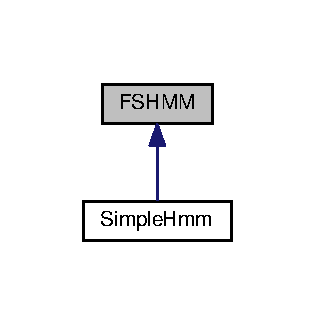
\includegraphics[width=151pt]{classFSHMM__inherit__graph}
\end{center}
\end{figure}
\subsection*{Public Member Functions}
\begin{DoxyCompactItemize}
\item 
\hyperlink{classFSHMM_a7d9109a5f787b3842f84257b79791cb9}{F\+S\+H\+MM} ()
\begin{DoxyCompactList}\small\item\em Default constructor (need this for resampling function) \end{DoxyCompactList}\item 
\hyperlink{classFSHMM_a644606d0cb00e2e0779fe8dcf53e2a42}{F\+S\+H\+MM} (const \hyperlink{pmfs_8h_a4c7df05c6f5e8a0d15ae14bcdbc07152}{Vec} \&init\+State\+Distr, const \hyperlink{pmfs_8h_ae601f56a556993079f730483c574356f}{Mat} \&trans\+Mat)
\begin{DoxyCompactList}\small\item\em Constructor. \end{DoxyCompactList}\item 
\hyperlink{classFSHMM_a0d011b77cf9541a312fffa43d24fa41f}{$\sim$\+F\+S\+H\+MM} ()\hypertarget{classFSHMM_a0d011b77cf9541a312fffa43d24fa41f}{}\label{classFSHMM_a0d011b77cf9541a312fffa43d24fa41f}

\begin{DoxyCompactList}\small\item\em Destructor. \end{DoxyCompactList}\item 
double \hyperlink{classFSHMM_a38325b38c4f20521f50cc7891d44839d}{get\+Cond\+Like} () const 
\begin{DoxyCompactList}\small\item\em Get the latest conditional likelihood. \end{DoxyCompactList}\item 
\hyperlink{pmfs_8h_a4c7df05c6f5e8a0d15ae14bcdbc07152}{Vec} \hyperlink{classFSHMM_af58a522cbeb2afa6a9211ac75100c1c2}{get\+Filter\+Vec} () const 
\begin{DoxyCompactList}\small\item\em Get the current filter vector. \end{DoxyCompactList}\item 
unsigned \hyperlink{classFSHMM_a2f166ff74c89b2103477be60eeb098d1}{dim\+State} () const 
\begin{DoxyCompactList}\small\item\em Get the dimension of the state. \end{DoxyCompactList}\item 
void \hyperlink{classFSHMM_a3e8519b8370eecec760d098bb5d38b3e}{update} (const \hyperlink{pmfs_8h_a4c7df05c6f5e8a0d15ae14bcdbc07152}{Vec} \&cond\+Dens\+Vec)
\begin{DoxyCompactList}\small\item\em Perform a H\+MM filter update. \end{DoxyCompactList}\end{DoxyCompactItemize}


\subsection{Detailed Description}
A base-\/class for Finite State H\+MM Filtering. 

Inherit from this if your model is a finite state hidden Markov model. 

\subsection{Constructor \& Destructor Documentation}
\index{F\+S\+H\+MM@{F\+S\+H\+MM}!F\+S\+H\+MM@{F\+S\+H\+MM}}
\index{F\+S\+H\+MM@{F\+S\+H\+MM}!F\+S\+H\+MM@{F\+S\+H\+MM}}
\subsubsection[{\texorpdfstring{F\+S\+H\+M\+M()}{FSHMM()}}]{\setlength{\rightskip}{0pt plus 5cm}F\+S\+H\+M\+M\+::\+F\+S\+H\+MM (
\begin{DoxyParamCaption}
{}
\end{DoxyParamCaption}
)}\hypertarget{classFSHMM_a7d9109a5f787b3842f84257b79791cb9}{}\label{classFSHMM_a7d9109a5f787b3842f84257b79791cb9}


Default constructor (need this for resampling function) 

Default constructor (need this for resampling function) \index{F\+S\+H\+MM@{F\+S\+H\+MM}!F\+S\+H\+MM@{F\+S\+H\+MM}}
\index{F\+S\+H\+MM@{F\+S\+H\+MM}!F\+S\+H\+MM@{F\+S\+H\+MM}}
\subsubsection[{\texorpdfstring{F\+S\+H\+M\+M(const Vec \&init\+State\+Distr, const Mat \&trans\+Mat)}{FSHMM(const Vec &initStateDistr, const Mat &transMat)}}]{\setlength{\rightskip}{0pt plus 5cm}F\+S\+H\+M\+M\+::\+F\+S\+H\+MM (
\begin{DoxyParamCaption}
\item[{const {\bf Vec} \&}]{init\+State\+Distr, }
\item[{const {\bf Mat} \&}]{trans\+Mat}
\end{DoxyParamCaption}
)}\hypertarget{classFSHMM_a644606d0cb00e2e0779fe8dcf53e2a42}{}\label{classFSHMM_a644606d0cb00e2e0779fe8dcf53e2a42}


Constructor. 


\begin{DoxyParams}{Parameters}
{\em init\+State\+Distr} & first time state prior distribution. \\
\hline
{\em trans\+Mat} & time homogeneous transition matrix. \\
\hline
\end{DoxyParams}


\subsection{Member Function Documentation}
\index{F\+S\+H\+MM@{F\+S\+H\+MM}!dim\+State@{dim\+State}}
\index{dim\+State@{dim\+State}!F\+S\+H\+MM@{F\+S\+H\+MM}}
\subsubsection[{\texorpdfstring{dim\+State() const }{dimState() const }}]{\setlength{\rightskip}{0pt plus 5cm}unsigned F\+S\+H\+M\+M\+::dim\+State (
\begin{DoxyParamCaption}
{}
\end{DoxyParamCaption}
) const}\hypertarget{classFSHMM_a2f166ff74c89b2103477be60eeb098d1}{}\label{classFSHMM_a2f166ff74c89b2103477be60eeb098d1}


Get the dimension of the state. 

Returns the dimension of the state process. \index{F\+S\+H\+MM@{F\+S\+H\+MM}!get\+Cond\+Like@{get\+Cond\+Like}}
\index{get\+Cond\+Like@{get\+Cond\+Like}!F\+S\+H\+MM@{F\+S\+H\+MM}}
\subsubsection[{\texorpdfstring{get\+Cond\+Like() const }{getCondLike() const }}]{\setlength{\rightskip}{0pt plus 5cm}double F\+S\+H\+M\+M\+::get\+Cond\+Like (
\begin{DoxyParamCaption}
{}
\end{DoxyParamCaption}
) const}\hypertarget{classFSHMM_a38325b38c4f20521f50cc7891d44839d}{}\label{classFSHMM_a38325b38c4f20521f50cc7891d44839d}


Get the latest conditional likelihood. 

\begin{DoxyReturn}{Returns}
the latest conditional likelihood. 
\end{DoxyReturn}
\index{F\+S\+H\+MM@{F\+S\+H\+MM}!get\+Filter\+Vec@{get\+Filter\+Vec}}
\index{get\+Filter\+Vec@{get\+Filter\+Vec}!F\+S\+H\+MM@{F\+S\+H\+MM}}
\subsubsection[{\texorpdfstring{get\+Filter\+Vec() const }{getFilterVec() const }}]{\setlength{\rightskip}{0pt plus 5cm}{\bf Vec} F\+S\+H\+M\+M\+::get\+Filter\+Vec (
\begin{DoxyParamCaption}
{}
\end{DoxyParamCaption}
) const}\hypertarget{classFSHMM_af58a522cbeb2afa6a9211ac75100c1c2}{}\label{classFSHMM_af58a522cbeb2afa6a9211ac75100c1c2}


Get the current filter vector. 

get the current filter vector. \begin{DoxyReturn}{Returns}
a probability Eigen\+::\+Vector\+Xd 
\end{DoxyReturn}
\index{F\+S\+H\+MM@{F\+S\+H\+MM}!update@{update}}
\index{update@{update}!F\+S\+H\+MM@{F\+S\+H\+MM}}
\subsubsection[{\texorpdfstring{update(const Vec \&cond\+Dens\+Vec)}{update(const Vec &condDensVec)}}]{\setlength{\rightskip}{0pt plus 5cm}void F\+S\+H\+M\+M\+::update (
\begin{DoxyParamCaption}
\item[{const {\bf Vec} \&}]{cond\+Dens\+Vec}
\end{DoxyParamCaption}
)}\hypertarget{classFSHMM_a3e8519b8370eecec760d098bb5d38b3e}{}\label{classFSHMM_a3e8519b8370eecec760d098bb5d38b3e}


Perform a H\+MM filter update. 

Perform a H\+MM filter update. 
\begin{DoxyParams}{Parameters}
{\em cond\+Dens\+Vec} & the vector (in x\+\_\+t) of p(y\+\_\+t$\vert$x\+\_\+t) \\
\hline
\end{DoxyParams}


The documentation for this class was generated from the following file\+:\begin{DoxyCompactItemize}
\item 
include/fshmm.\+h\end{DoxyCompactItemize}

\hypertarget{classHmm__Rbpf}{}\section{Hmm\+\_\+\+Rbpf$<$ np $>$ Class Template Reference}
\label{classHmm__Rbpf}\index{Hmm\+\_\+\+Rbpf$<$ np $>$@{Hmm\+\_\+\+Rbpf$<$ np $>$}}


A base-\/class for H\+MM Rao-\/\+Blackwellized Particle Filtering.  




{\ttfamily \#include $<$hmm\+\_\+rbpf\+\_\+sisr.\+h$>$}

\subsection*{Public Member Functions}
\begin{DoxyCompactItemize}
\item 
\hyperlink{classHmm__Rbpf_a5f6b635ecde176edefd4709132a49f74}{Hmm\+\_\+\+Rbpf} (\hyperlink{hmm__rbpf__sisr_8h_aa0729d190f1f8b76b203466a41f1505f}{H\+M\+M\+R\+B\+P\+F\+Resamp\+Style} rt=H\+M\+M\+R\+B\+P\+F\+Resamp\+Style\+::everytime\+\_\+multinomial)
\begin{DoxyCompactList}\small\item\em The constructor. \end{DoxyCompactList}\item 
\hyperlink{classHmm__Rbpf_a6a5a602ca9be58ac12a4fb2545ebd2cc}{$\sim$\+Hmm\+\_\+\+Rbpf} ()
\begin{DoxyCompactList}\small\item\em Destructor. \end{DoxyCompactList}\item 
void \hyperlink{classHmm__Rbpf_a874a9cbd4cb5d6c3961624bb3e08fa4c}{filter} (const \hyperlink{apf__filter_8h_a4c7df05c6f5e8a0d15ae14bcdbc07152}{Vec} \&data, const std\+::vector$<$ std\+::function$<$ const \hyperlink{apf__filter_8h_ae601f56a556993079f730483c574356f}{Mat}(const \hyperlink{apf__filter_8h_a4c7df05c6f5e8a0d15ae14bcdbc07152}{Vec} \&x1t\+Probs, const \hyperlink{apf__filter_8h_a4c7df05c6f5e8a0d15ae14bcdbc07152}{Vec} \&x2t)$>$ $>$ \&fs=std\+::vector$<$ std\+::function$<$ const \hyperlink{apf__filter_8h_ae601f56a556993079f730483c574356f}{Mat}(const \hyperlink{apf__filter_8h_a4c7df05c6f5e8a0d15ae14bcdbc07152}{Vec} \&, const \hyperlink{apf__filter_8h_a4c7df05c6f5e8a0d15ae14bcdbc07152}{Vec} \&)$>$ $>$())
\begin{DoxyCompactList}\small\item\em Filter. \end{DoxyCompactList}\item 
double \hyperlink{classHmm__Rbpf_a39ddb0a59bce678e13fc04f2b394c36d}{get\+Log\+Cond\+Like} () const 
\begin{DoxyCompactList}\small\item\em Get the latest conditional likelihood. \end{DoxyCompactList}\item 
std\+::vector$<$ \hyperlink{apf__filter_8h_ae601f56a556993079f730483c574356f}{Mat} $>$ \hyperlink{classHmm__Rbpf_a4e8cd1a8d1d56e70cf2eee2f24925953}{get\+Expectations} () const 
\begin{DoxyCompactList}\small\item\em Get vector of expectations. \end{DoxyCompactList}\item 
virtual double \hyperlink{classHmm__Rbpf_aecfbf4f24599accbf2bbda77de8d1b99}{log\+Mu\+Ev} (const \hyperlink{apf__filter_8h_a4c7df05c6f5e8a0d15ae14bcdbc07152}{Vec} \&x21)=0
\begin{DoxyCompactList}\small\item\em Evaluates the first time state density. \end{DoxyCompactList}\item 
virtual \hyperlink{apf__filter_8h_a4c7df05c6f5e8a0d15ae14bcdbc07152}{Vec} \hyperlink{classHmm__Rbpf_a95f6f299b49e8c47993fab2772a517b4}{q1\+Samp} (const \hyperlink{apf__filter_8h_a4c7df05c6f5e8a0d15ae14bcdbc07152}{Vec} \&y1)=0
\begin{DoxyCompactList}\small\item\em Sample from the first sampler. \end{DoxyCompactList}\item 
virtual \hyperlink{apf__filter_8h_a4c7df05c6f5e8a0d15ae14bcdbc07152}{Vec} \hyperlink{classHmm__Rbpf_a22bf131a47a9e96e39b6bbb5f60e597d}{init\+H\+M\+M\+Prob\+Vec} (const \hyperlink{apf__filter_8h_a4c7df05c6f5e8a0d15ae14bcdbc07152}{Vec} \&x21)=0
\begin{DoxyCompactList}\small\item\em Provides the initial mean vector for each H\+MM filter object. \end{DoxyCompactList}\item 
virtual \hyperlink{apf__filter_8h_ae601f56a556993079f730483c574356f}{Mat} \hyperlink{classHmm__Rbpf_a455f785b1283acce5e01a80c58dd350d}{init\+H\+M\+M\+Trans\+Mat} (const \hyperlink{apf__filter_8h_a4c7df05c6f5e8a0d15ae14bcdbc07152}{Vec} \&x21)=0
\begin{DoxyCompactList}\small\item\em Provides the transition matrix for each H\+MM filter object. \end{DoxyCompactList}\item 
virtual \hyperlink{apf__filter_8h_a4c7df05c6f5e8a0d15ae14bcdbc07152}{Vec} \hyperlink{classHmm__Rbpf_a2394e61d4b4c25b0f6956804625845d4}{q\+Samp} (const \hyperlink{apf__filter_8h_a4c7df05c6f5e8a0d15ae14bcdbc07152}{Vec} \&x2tm1, const \hyperlink{apf__filter_8h_a4c7df05c6f5e8a0d15ae14bcdbc07152}{Vec} \&yt)=0
\begin{DoxyCompactList}\small\item\em Samples the time t second component. \end{DoxyCompactList}\item 
virtual double \hyperlink{classHmm__Rbpf_a6b7d654499d59cff3333ff068fc05f00}{log\+Q1\+Ev} (const \hyperlink{apf__filter_8h_a4c7df05c6f5e8a0d15ae14bcdbc07152}{Vec} \&x21, const \hyperlink{apf__filter_8h_a4c7df05c6f5e8a0d15ae14bcdbc07152}{Vec} \&y1)=0
\begin{DoxyCompactList}\small\item\em Evaluates the proposal density of the second state component at time 1. \end{DoxyCompactList}\item 
virtual double \hyperlink{classHmm__Rbpf_a2225a77385e1c741cd49e2f05e432ca9}{log\+F\+Ev} (const \hyperlink{apf__filter_8h_a4c7df05c6f5e8a0d15ae14bcdbc07152}{Vec} \&x2t, const \hyperlink{apf__filter_8h_a4c7df05c6f5e8a0d15ae14bcdbc07152}{Vec} \&x2tm1)=0
\begin{DoxyCompactList}\small\item\em Evaluates the state transition density for the second state component. \end{DoxyCompactList}\item 
virtual double \hyperlink{classHmm__Rbpf_a60b56c34a56e3a9090fb4f705f0bdde1}{log\+Q\+Ev} (const \hyperlink{apf__filter_8h_a4c7df05c6f5e8a0d15ae14bcdbc07152}{Vec} \&x2t, const \hyperlink{apf__filter_8h_a4c7df05c6f5e8a0d15ae14bcdbc07152}{Vec} \&x2tm1, const \hyperlink{apf__filter_8h_a4c7df05c6f5e8a0d15ae14bcdbc07152}{Vec} \&yt)=0
\begin{DoxyCompactList}\small\item\em Evaluates the proposal density at time t $>$ 1. \end{DoxyCompactList}\item 
virtual void \hyperlink{classHmm__Rbpf_a3ca8ae39c7d1c52ceaf300b6b2564edf}{update\+F\+S\+H\+MM} (\hyperlink{classFSHMM}{F\+S\+H\+MM} \&a\+Model, const \hyperlink{apf__filter_8h_a4c7df05c6f5e8a0d15ae14bcdbc07152}{Vec} \&yt, const \hyperlink{apf__filter_8h_a4c7df05c6f5e8a0d15ae14bcdbc07152}{Vec} \&x2t)=0
\begin{DoxyCompactList}\small\item\em How to update your inner H\+MM filter object at each time. \end{DoxyCompactList}\end{DoxyCompactItemize}


\subsection{Detailed Description}
\subsubsection*{template$<$size\+\_\+t np$>$\\*
class Hmm\+\_\+\+Rbpf$<$ np $>$}

A base-\/class for H\+MM Rao-\/\+Blackwellized Particle Filtering. 

\begin{DoxyAuthor}{Author}
taylor 
\end{DoxyAuthor}


\subsection{Constructor \& Destructor Documentation}
\index{Hmm\+\_\+\+Rbpf@{Hmm\+\_\+\+Rbpf}!Hmm\+\_\+\+Rbpf@{Hmm\+\_\+\+Rbpf}}
\index{Hmm\+\_\+\+Rbpf@{Hmm\+\_\+\+Rbpf}!Hmm\+\_\+\+Rbpf@{Hmm\+\_\+\+Rbpf}}
\subsubsection[{\texorpdfstring{Hmm\+\_\+\+Rbpf(\+H\+M\+M\+R\+B\+P\+F\+Resamp\+Style rt=\+H\+M\+M\+R\+B\+P\+F\+Resamp\+Style\+::everytime\+\_\+multinomial)}{Hmm_Rbpf(HMMRBPFResampStyle rt=HMMRBPFResampStyle::everytime_multinomial)}}]{\setlength{\rightskip}{0pt plus 5cm}template$<$size\+\_\+t np$>$ {\bf Hmm\+\_\+\+Rbpf}$<$ np $>$\+::{\bf Hmm\+\_\+\+Rbpf} (
\begin{DoxyParamCaption}
\item[{{\bf H\+M\+M\+R\+B\+P\+F\+Resamp\+Style}}]{rt = {\ttfamily HMMRBPFResampStyle\+:\+:everytime\+\_\+multinomial}}
\end{DoxyParamCaption}
)}\hypertarget{classHmm__Rbpf_a5f6b635ecde176edefd4709132a49f74}{}\label{classHmm__Rbpf_a5f6b635ecde176edefd4709132a49f74}


The constructor. 

constructor. 
\begin{DoxyParams}{Parameters}
{\em rt} & the type of resampling you want to do. \\
\hline
\end{DoxyParams}
\index{Hmm\+\_\+\+Rbpf@{Hmm\+\_\+\+Rbpf}!````~Hmm\+\_\+\+Rbpf@{$\sim$\+Hmm\+\_\+\+Rbpf}}
\index{````~Hmm\+\_\+\+Rbpf@{$\sim$\+Hmm\+\_\+\+Rbpf}!Hmm\+\_\+\+Rbpf@{Hmm\+\_\+\+Rbpf}}
\subsubsection[{\texorpdfstring{$\sim$\+Hmm\+\_\+\+Rbpf()}{~Hmm_Rbpf()}}]{\setlength{\rightskip}{0pt plus 5cm}template$<$size\+\_\+t np$>$ {\bf Hmm\+\_\+\+Rbpf}$<$ np $>$\+::$\sim${\bf Hmm\+\_\+\+Rbpf} (
\begin{DoxyParamCaption}
{}
\end{DoxyParamCaption}
)}\hypertarget{classHmm__Rbpf_a6a5a602ca9be58ac12a4fb2545ebd2cc}{}\label{classHmm__Rbpf_a6a5a602ca9be58ac12a4fb2545ebd2cc}


Destructor. 

destructor. 

\subsection{Member Function Documentation}
\index{Hmm\+\_\+\+Rbpf@{Hmm\+\_\+\+Rbpf}!filter@{filter}}
\index{filter@{filter}!Hmm\+\_\+\+Rbpf@{Hmm\+\_\+\+Rbpf}}
\subsubsection[{\texorpdfstring{filter(const Vec \&data, const std\+::vector$<$ std\+::function$<$ const Mat(const Vec \&x1t\+Probs, const Vec \&x2t)$>$ $>$ \&fs=std\+::vector$<$ std\+::function$<$ const Mat(const Vec \&, const Vec \&)$>$ $>$())}{filter(const Vec &data, const std::vector< std::function< const Mat(const Vec &x1tProbs, const Vec &x2t)> > &fs=std::vector< std::function< const Mat(const Vec &, const Vec &)> >())}}]{\setlength{\rightskip}{0pt plus 5cm}template$<$size\+\_\+t np$>$ void {\bf Hmm\+\_\+\+Rbpf}$<$ np $>$\+::filter (
\begin{DoxyParamCaption}
\item[{const {\bf Vec} \&}]{data, }
\item[{const std\+::vector$<$ std\+::function$<$ const {\bf Mat}(const {\bf Vec} \&x1t\+Probs, const {\bf Vec} \&x2t)$>$ $>$ \&}]{fs = {\ttfamily std\+:\+:vector$<$std\+:\+:function$<$const~{\bf Mat}(const~{\bf Vec}\&,~const~{\bf Vec}\&)$>$~$>$()}}
\end{DoxyParamCaption}
)}\hypertarget{classHmm__Rbpf_a874a9cbd4cb5d6c3961624bb3e08fa4c}{}\label{classHmm__Rbpf_a874a9cbd4cb5d6c3961624bb3e08fa4c}


Filter. 

filters everything based on a new data point. 
\begin{DoxyParams}{Parameters}
{\em data} & the most recent time series observation. \\
\hline
{\em fs} & a vector of functions computing E\mbox{[}h(x\+\_\+1t, x\+\_\+2t$^\wedge$i)$\vert$ x\+\_\+2t$^\wedge$i,y\+\_\+1\+:t\mbox{]}. Will access the probability vector of x\+\_\+1t \\
\hline
\end{DoxyParams}
\index{Hmm\+\_\+\+Rbpf@{Hmm\+\_\+\+Rbpf}!get\+Expectations@{get\+Expectations}}
\index{get\+Expectations@{get\+Expectations}!Hmm\+\_\+\+Rbpf@{Hmm\+\_\+\+Rbpf}}
\subsubsection[{\texorpdfstring{get\+Expectations() const }{getExpectations() const }}]{\setlength{\rightskip}{0pt plus 5cm}template$<$size\+\_\+t np$>$ std\+::vector$<$ {\bf Mat} $>$ {\bf Hmm\+\_\+\+Rbpf}$<$ np $>$\+::get\+Expectations (
\begin{DoxyParamCaption}
{}
\end{DoxyParamCaption}
) const}\hypertarget{classHmm__Rbpf_a4e8cd1a8d1d56e70cf2eee2f24925953}{}\label{classHmm__Rbpf_a4e8cd1a8d1d56e70cf2eee2f24925953}


Get vector of expectations. 

\begin{DoxyReturn}{Returns}
vector of expectations 
\end{DoxyReturn}
\index{Hmm\+\_\+\+Rbpf@{Hmm\+\_\+\+Rbpf}!get\+Log\+Cond\+Like@{get\+Log\+Cond\+Like}}
\index{get\+Log\+Cond\+Like@{get\+Log\+Cond\+Like}!Hmm\+\_\+\+Rbpf@{Hmm\+\_\+\+Rbpf}}
\subsubsection[{\texorpdfstring{get\+Log\+Cond\+Like() const }{getLogCondLike() const }}]{\setlength{\rightskip}{0pt plus 5cm}template$<$size\+\_\+t np$>$ double {\bf Hmm\+\_\+\+Rbpf}$<$ np $>$\+::get\+Log\+Cond\+Like (
\begin{DoxyParamCaption}
{}
\end{DoxyParamCaption}
) const}\hypertarget{classHmm__Rbpf_a39ddb0a59bce678e13fc04f2b394c36d}{}\label{classHmm__Rbpf_a39ddb0a59bce678e13fc04f2b394c36d}


Get the latest conditional likelihood. 

Get the latest conditional likelihood. \begin{DoxyReturn}{Returns}
the latest conditional likelihood. 
\end{DoxyReturn}
\index{Hmm\+\_\+\+Rbpf@{Hmm\+\_\+\+Rbpf}!init\+H\+M\+M\+Prob\+Vec@{init\+H\+M\+M\+Prob\+Vec}}
\index{init\+H\+M\+M\+Prob\+Vec@{init\+H\+M\+M\+Prob\+Vec}!Hmm\+\_\+\+Rbpf@{Hmm\+\_\+\+Rbpf}}
\subsubsection[{\texorpdfstring{init\+H\+M\+M\+Prob\+Vec(const Vec \&x21)=0}{initHMMProbVec(const Vec &x21)=0}}]{\setlength{\rightskip}{0pt plus 5cm}template$<$size\+\_\+t np$>$ virtual {\bf Vec} {\bf Hmm\+\_\+\+Rbpf}$<$ np $>$\+::init\+H\+M\+M\+Prob\+Vec (
\begin{DoxyParamCaption}
\item[{const {\bf Vec} \&}]{x21}
\end{DoxyParamCaption}
)\hspace{0.3cm}{\ttfamily [pure virtual]}}\hypertarget{classHmm__Rbpf_a22bf131a47a9e96e39b6bbb5f60e597d}{}\label{classHmm__Rbpf_a22bf131a47a9e96e39b6bbb5f60e597d}


Provides the initial mean vector for each H\+MM filter object. 

provides the initial probability vector for each H\+MM filter object. 
\begin{DoxyParams}{Parameters}
{\em x21} & the second state componenent at time 1. \\
\hline
\end{DoxyParams}
\begin{DoxyReturn}{Returns}
a Vec representing the probability of each state element. 
\end{DoxyReturn}
\index{Hmm\+\_\+\+Rbpf@{Hmm\+\_\+\+Rbpf}!init\+H\+M\+M\+Trans\+Mat@{init\+H\+M\+M\+Trans\+Mat}}
\index{init\+H\+M\+M\+Trans\+Mat@{init\+H\+M\+M\+Trans\+Mat}!Hmm\+\_\+\+Rbpf@{Hmm\+\_\+\+Rbpf}}
\subsubsection[{\texorpdfstring{init\+H\+M\+M\+Trans\+Mat(const Vec \&x21)=0}{initHMMTransMat(const Vec &x21)=0}}]{\setlength{\rightskip}{0pt plus 5cm}template$<$size\+\_\+t np$>$ virtual {\bf Mat} {\bf Hmm\+\_\+\+Rbpf}$<$ np $>$\+::init\+H\+M\+M\+Trans\+Mat (
\begin{DoxyParamCaption}
\item[{const {\bf Vec} \&}]{x21}
\end{DoxyParamCaption}
)\hspace{0.3cm}{\ttfamily [pure virtual]}}\hypertarget{classHmm__Rbpf_a455f785b1283acce5e01a80c58dd350d}{}\label{classHmm__Rbpf_a455f785b1283acce5e01a80c58dd350d}


Provides the transition matrix for each H\+MM filter object. 

provides the transition matrix for each H\+MM filter object. 
\begin{DoxyParams}{Parameters}
{\em x21} & the second state component at time 1. \\
\hline
\end{DoxyParams}
\begin{DoxyReturn}{Returns}
a transition matrix where element (ij) is the probability of transitioning from state i to state j. 
\end{DoxyReturn}
\index{Hmm\+\_\+\+Rbpf@{Hmm\+\_\+\+Rbpf}!log\+F\+Ev@{log\+F\+Ev}}
\index{log\+F\+Ev@{log\+F\+Ev}!Hmm\+\_\+\+Rbpf@{Hmm\+\_\+\+Rbpf}}
\subsubsection[{\texorpdfstring{log\+F\+Ev(const Vec \&x2t, const Vec \&x2tm1)=0}{logFEv(const Vec &x2t, const Vec &x2tm1)=0}}]{\setlength{\rightskip}{0pt plus 5cm}template$<$size\+\_\+t np$>$ virtual double {\bf Hmm\+\_\+\+Rbpf}$<$ np $>$\+::log\+F\+Ev (
\begin{DoxyParamCaption}
\item[{const {\bf Vec} \&}]{x2t, }
\item[{const {\bf Vec} \&}]{x2tm1}
\end{DoxyParamCaption}
)\hspace{0.3cm}{\ttfamily [pure virtual]}}\hypertarget{classHmm__Rbpf_a2225a77385e1c741cd49e2f05e432ca9}{}\label{classHmm__Rbpf_a2225a77385e1c741cd49e2f05e432ca9}


Evaluates the state transition density for the second state component. 

Evaluates the state transition density for the second state component. 
\begin{DoxyParams}{Parameters}
{\em x2t} & the current second state component. \\
\hline
{\em x2tm1} & the previous second state component. \\
\hline
\end{DoxyParams}
\begin{DoxyReturn}{Returns}
a double evaluation. 
\end{DoxyReturn}
\index{Hmm\+\_\+\+Rbpf@{Hmm\+\_\+\+Rbpf}!log\+Mu\+Ev@{log\+Mu\+Ev}}
\index{log\+Mu\+Ev@{log\+Mu\+Ev}!Hmm\+\_\+\+Rbpf@{Hmm\+\_\+\+Rbpf}}
\subsubsection[{\texorpdfstring{log\+Mu\+Ev(const Vec \&x21)=0}{logMuEv(const Vec &x21)=0}}]{\setlength{\rightskip}{0pt plus 5cm}template$<$size\+\_\+t np$>$ virtual double {\bf Hmm\+\_\+\+Rbpf}$<$ np $>$\+::log\+Mu\+Ev (
\begin{DoxyParamCaption}
\item[{const {\bf Vec} \&}]{x21}
\end{DoxyParamCaption}
)\hspace{0.3cm}{\ttfamily [pure virtual]}}\hypertarget{classHmm__Rbpf_aecfbf4f24599accbf2bbda77de8d1b99}{}\label{classHmm__Rbpf_aecfbf4f24599accbf2bbda77de8d1b99}


Evaluates the first time state density. 

evaluates mu. 
\begin{DoxyParams}{Parameters}
{\em x21} & component two at time 1 \\
\hline
\end{DoxyParams}
\begin{DoxyReturn}{Returns}
a double evaluation 
\end{DoxyReturn}
\index{Hmm\+\_\+\+Rbpf@{Hmm\+\_\+\+Rbpf}!log\+Q1\+Ev@{log\+Q1\+Ev}}
\index{log\+Q1\+Ev@{log\+Q1\+Ev}!Hmm\+\_\+\+Rbpf@{Hmm\+\_\+\+Rbpf}}
\subsubsection[{\texorpdfstring{log\+Q1\+Ev(const Vec \&x21, const Vec \&y1)=0}{logQ1Ev(const Vec &x21, const Vec &y1)=0}}]{\setlength{\rightskip}{0pt plus 5cm}template$<$size\+\_\+t np$>$ virtual double {\bf Hmm\+\_\+\+Rbpf}$<$ np $>$\+::log\+Q1\+Ev (
\begin{DoxyParamCaption}
\item[{const {\bf Vec} \&}]{x21, }
\item[{const {\bf Vec} \&}]{y1}
\end{DoxyParamCaption}
)\hspace{0.3cm}{\ttfamily [pure virtual]}}\hypertarget{classHmm__Rbpf_a6b7d654499d59cff3333ff068fc05f00}{}\label{classHmm__Rbpf_a6b7d654499d59cff3333ff068fc05f00}


Evaluates the proposal density of the second state component at time 1. 

Evaluates the proposal density of the second state component at time 1. 
\begin{DoxyParams}{Parameters}
{\em x21} & the second state component at time 1 you sampled. \\
\hline
{\em y1} & time 1 observation. \\
\hline
\end{DoxyParams}
\begin{DoxyReturn}{Returns}
a double evaluation of the density. 
\end{DoxyReturn}
\index{Hmm\+\_\+\+Rbpf@{Hmm\+\_\+\+Rbpf}!log\+Q\+Ev@{log\+Q\+Ev}}
\index{log\+Q\+Ev@{log\+Q\+Ev}!Hmm\+\_\+\+Rbpf@{Hmm\+\_\+\+Rbpf}}
\subsubsection[{\texorpdfstring{log\+Q\+Ev(const Vec \&x2t, const Vec \&x2tm1, const Vec \&yt)=0}{logQEv(const Vec &x2t, const Vec &x2tm1, const Vec &yt)=0}}]{\setlength{\rightskip}{0pt plus 5cm}template$<$size\+\_\+t np$>$ virtual double {\bf Hmm\+\_\+\+Rbpf}$<$ np $>$\+::log\+Q\+Ev (
\begin{DoxyParamCaption}
\item[{const {\bf Vec} \&}]{x2t, }
\item[{const {\bf Vec} \&}]{x2tm1, }
\item[{const {\bf Vec} \&}]{yt}
\end{DoxyParamCaption}
)\hspace{0.3cm}{\ttfamily [pure virtual]}}\hypertarget{classHmm__Rbpf_a60b56c34a56e3a9090fb4f705f0bdde1}{}\label{classHmm__Rbpf_a60b56c34a56e3a9090fb4f705f0bdde1}


Evaluates the proposal density at time t $>$ 1. 

Evaluates the proposal density at time t $>$ 1. 
\begin{DoxyParams}{Parameters}
{\em x2t} & the current second state component. \\
\hline
{\em x2tm1} & the previous second state component. \\
\hline
{\em yt} & the current time series observation. \\
\hline
\end{DoxyParams}
\begin{DoxyReturn}{Returns}
a double evaluation. 
\end{DoxyReturn}
\index{Hmm\+\_\+\+Rbpf@{Hmm\+\_\+\+Rbpf}!q1\+Samp@{q1\+Samp}}
\index{q1\+Samp@{q1\+Samp}!Hmm\+\_\+\+Rbpf@{Hmm\+\_\+\+Rbpf}}
\subsubsection[{\texorpdfstring{q1\+Samp(const Vec \&y1)=0}{q1Samp(const Vec &y1)=0}}]{\setlength{\rightskip}{0pt plus 5cm}template$<$size\+\_\+t np$>$ virtual {\bf Vec} {\bf Hmm\+\_\+\+Rbpf}$<$ np $>$\+::q1\+Samp (
\begin{DoxyParamCaption}
\item[{const {\bf Vec} \&}]{y1}
\end{DoxyParamCaption}
)\hspace{0.3cm}{\ttfamily [pure virtual]}}\hypertarget{classHmm__Rbpf_a95f6f299b49e8c47993fab2772a517b4}{}\label{classHmm__Rbpf_a95f6f299b49e8c47993fab2772a517b4}


Sample from the first sampler. 

samples the second component of the state at time 1. 
\begin{DoxyParams}{Parameters}
{\em y1} & most recent datum. \\
\hline
\end{DoxyParams}
\begin{DoxyReturn}{Returns}
a Vec sample for x21. 
\end{DoxyReturn}
\index{Hmm\+\_\+\+Rbpf@{Hmm\+\_\+\+Rbpf}!q\+Samp@{q\+Samp}}
\index{q\+Samp@{q\+Samp}!Hmm\+\_\+\+Rbpf@{Hmm\+\_\+\+Rbpf}}
\subsubsection[{\texorpdfstring{q\+Samp(const Vec \&x2tm1, const Vec \&yt)=0}{qSamp(const Vec &x2tm1, const Vec &yt)=0}}]{\setlength{\rightskip}{0pt plus 5cm}template$<$size\+\_\+t np$>$ virtual {\bf Vec} {\bf Hmm\+\_\+\+Rbpf}$<$ np $>$\+::q\+Samp (
\begin{DoxyParamCaption}
\item[{const {\bf Vec} \&}]{x2tm1, }
\item[{const {\bf Vec} \&}]{yt}
\end{DoxyParamCaption}
)\hspace{0.3cm}{\ttfamily [pure virtual]}}\hypertarget{classHmm__Rbpf_a2394e61d4b4c25b0f6956804625845d4}{}\label{classHmm__Rbpf_a2394e61d4b4c25b0f6956804625845d4}


Samples the time t second component. 

Samples the time t second component. 
\begin{DoxyParams}{Parameters}
{\em x2tm1} & the previous time\textquotesingle{}s second state component. \\
\hline
{\em yt} & the current observation. \\
\hline
\end{DoxyParams}
\begin{DoxyReturn}{Returns}
a Vec sample of the second state component at the current time. 
\end{DoxyReturn}
\index{Hmm\+\_\+\+Rbpf@{Hmm\+\_\+\+Rbpf}!update\+F\+S\+H\+MM@{update\+F\+S\+H\+MM}}
\index{update\+F\+S\+H\+MM@{update\+F\+S\+H\+MM}!Hmm\+\_\+\+Rbpf@{Hmm\+\_\+\+Rbpf}}
\subsubsection[{\texorpdfstring{update\+F\+S\+H\+M\+M(\+F\+S\+H\+M\+M \&a\+Model, const Vec \&yt, const Vec \&x2t)=0}{updateFSHMM(FSHMM &aModel, const Vec &yt, const Vec &x2t)=0}}]{\setlength{\rightskip}{0pt plus 5cm}template$<$size\+\_\+t np$>$ virtual void {\bf Hmm\+\_\+\+Rbpf}$<$ np $>$\+::update\+F\+S\+H\+MM (
\begin{DoxyParamCaption}
\item[{{\bf F\+S\+H\+MM} \&}]{a\+Model, }
\item[{const {\bf Vec} \&}]{yt, }
\item[{const {\bf Vec} \&}]{x2t}
\end{DoxyParamCaption}
)\hspace{0.3cm}{\ttfamily [pure virtual]}}\hypertarget{classHmm__Rbpf_a3ca8ae39c7d1c52ceaf300b6b2564edf}{}\label{classHmm__Rbpf_a3ca8ae39c7d1c52ceaf300b6b2564edf}


How to update your inner H\+MM filter object at each time. 

How to update your inner H\+MM filter object at each time. 
\begin{DoxyParams}{Parameters}
{\em a\+Model} & a H\+MM filter object describing the conditional closed-\/form model. \\
\hline
{\em yt} & the current time series observation. \\
\hline
{\em x2t} & the current second state component. \\
\hline
\end{DoxyParams}


The documentation for this class was generated from the following file\+:\begin{DoxyCompactItemize}
\item 
include/\hyperlink{hmm__rbpf__sisr_8h}{hmm\+\_\+rbpf\+\_\+sisr.\+h}\end{DoxyCompactItemize}

\hypertarget{classKalman__RBPF}{}\section{Kalman\+\_\+\+R\+B\+PF Class Reference}
\label{classKalman__RBPF}\index{Kalman\+\_\+\+R\+B\+PF@{Kalman\+\_\+\+R\+B\+PF}}


A base-\/class for Kalman Rao-\/\+Blackwellized Particle Filtering.  




{\ttfamily \#include $<$kalman\+\_\+rbpf.\+h$>$}

\subsection*{Public Member Functions}
\begin{DoxyCompactItemize}
\item 
\hyperlink{classKalman__RBPF_aa7130565819b45f993100dbf7f048c37}{Kalman\+\_\+\+R\+B\+PF} (int num\+Parts, R\+B\+P\+F\+Resamp\+Style resamp\+Technique=R\+B\+P\+F\+Resamp\+Style\+::everytime\+\_\+multinomial)
\begin{DoxyCompactList}\small\item\em The constructor. \end{DoxyCompactList}\item 
\hyperlink{classKalman__RBPF_a454f1736e8889904f755ca904f6eebc0}{$\sim$\+Kalman\+\_\+\+R\+B\+PF} ()\hypertarget{classKalman__RBPF_a454f1736e8889904f755ca904f6eebc0}{}\label{classKalman__RBPF_a454f1736e8889904f755ca904f6eebc0}

\begin{DoxyCompactList}\small\item\em The desuctor. \end{DoxyCompactList}\item 
void \hyperlink{classKalman__RBPF_a72d5ed61d0289a6977bf178145f5b969}{filter} (const Vec \&data)
\begin{DoxyCompactList}\small\item\em Filter! \end{DoxyCompactList}\item 
double \hyperlink{classKalman__RBPF_a2d65ffce3d115ecaf1c8e97b9222cdde}{get\+Cond\+Like} () const 
\begin{DoxyCompactList}\small\item\em Get the latest conditional likelihood. \end{DoxyCompactList}\item 
std\+::vector$<$ double $>$ \hyperlink{classKalman__RBPF_a8d411f1992b9a09ac3ee70f48ed34c7c}{get\+Weights} () const 
\begin{DoxyCompactList}\small\item\em Get the up-\/to-\/date un-\/normalized weights. \end{DoxyCompactList}\item 
virtual double {\bfseries mu\+Ev} (const Vec \&x21)=0\hypertarget{classKalman__RBPF_a25e8682d13a04eb1075a4d30dfa6825a}{}\label{classKalman__RBPF_a25e8682d13a04eb1075a4d30dfa6825a}

\item 
virtual Vec {\bfseries q1\+Samp} (const Vec \&y1)=0\hypertarget{classKalman__RBPF_a71e394c093f606f80a92a3fc4fe087a3}{}\label{classKalman__RBPF_a71e394c093f606f80a92a3fc4fe087a3}

\item 
virtual Vec {\bfseries init\+Kalman\+Mean} (const Vec \&x21)=0\hypertarget{classKalman__RBPF_a870a53fc149adf8042fa12eb5d9a8d30}{}\label{classKalman__RBPF_a870a53fc149adf8042fa12eb5d9a8d30}

\item 
virtual Mat {\bfseries init\+Kalman\+Var} (const Vec \&x21)=0\hypertarget{classKalman__RBPF_a4f7f37a90d9382ca2ad7dfef4acf1bc0}{}\label{classKalman__RBPF_a4f7f37a90d9382ca2ad7dfef4acf1bc0}

\item 
virtual Vec {\bfseries q\+Samp} (const Vec \&x2tm1, const Vec \&yt)=0\hypertarget{classKalman__RBPF_ad3ee89a06a18a287445e366230a6bd65}{}\label{classKalman__RBPF_ad3ee89a06a18a287445e366230a6bd65}

\item 
virtual double {\bfseries q1\+Ev} (const Vec \&x1, const Vec \&y1)=0\hypertarget{classKalman__RBPF_abc3a0c0214699593426db94db29298d6}{}\label{classKalman__RBPF_abc3a0c0214699593426db94db29298d6}

\item 
virtual double {\bfseries f\+Ev} (const Vec \&x2t, const Vec \&x2tm1)=0\hypertarget{classKalman__RBPF_a03bfc2e7f32a86ab4fe653958d2f7dd4}{}\label{classKalman__RBPF_a03bfc2e7f32a86ab4fe653958d2f7dd4}

\item 
virtual double {\bfseries q\+Ev} (const Vec \&x2t, const Vec \&x2tm1, const Vec \&yt)=0\hypertarget{classKalman__RBPF_ad5b8e717c5d4c838b0d246b496971d16}{}\label{classKalman__RBPF_ad5b8e717c5d4c838b0d246b496971d16}

\item 
virtual void {\bfseries update\+Kalman} (\hyperlink{classLgssm}{Lgssm} \&a\+Model, const Vec \&yt, const Vec \&x2t)=0\hypertarget{classKalman__RBPF_a67abffa6fe0510147037ed102aa30ed0}{}\label{classKalman__RBPF_a67abffa6fe0510147037ed102aa30ed0}

\end{DoxyCompactItemize}


\subsection{Detailed Description}
A base-\/class for Kalman Rao-\/\+Blackwellized Particle Filtering. 

\begin{DoxyAuthor}{Author}
taylor 
\end{DoxyAuthor}


\subsection{Constructor \& Destructor Documentation}
\index{Kalman\+\_\+\+R\+B\+PF@{Kalman\+\_\+\+R\+B\+PF}!Kalman\+\_\+\+R\+B\+PF@{Kalman\+\_\+\+R\+B\+PF}}
\index{Kalman\+\_\+\+R\+B\+PF@{Kalman\+\_\+\+R\+B\+PF}!Kalman\+\_\+\+R\+B\+PF@{Kalman\+\_\+\+R\+B\+PF}}
\subsubsection[{\texorpdfstring{Kalman\+\_\+\+R\+B\+P\+F(int num\+Parts, R\+B\+P\+F\+Resamp\+Style resamp\+Technique=\+R\+B\+P\+F\+Resamp\+Style\+::everytime\+\_\+multinomial)}{Kalman_RBPF(int numParts, RBPFResampStyle resampTechnique=RBPFResampStyle::everytime_multinomial)}}]{\setlength{\rightskip}{0pt plus 5cm}Kalman\+\_\+\+R\+B\+P\+F\+::\+Kalman\+\_\+\+R\+B\+PF (
\begin{DoxyParamCaption}
\item[{int}]{num\+Parts, }
\item[{R\+B\+P\+F\+Resamp\+Style}]{resamp\+Technique = {\ttfamily RBPFResampStyle\+:\+:everytime\+\_\+multinomial}}
\end{DoxyParamCaption}
)}\hypertarget{classKalman__RBPF_aa7130565819b45f993100dbf7f048c37}{}\label{classKalman__RBPF_aa7130565819b45f993100dbf7f048c37}


The constructor. 


\begin{DoxyParams}{Parameters}
{\em num\+Parts} & the number of particles. \\
\hline
{\em resamp\+Technique} & the type of resampling you want to do. \\
\hline
\end{DoxyParams}


\subsection{Member Function Documentation}
\index{Kalman\+\_\+\+R\+B\+PF@{Kalman\+\_\+\+R\+B\+PF}!filter@{filter}}
\index{filter@{filter}!Kalman\+\_\+\+R\+B\+PF@{Kalman\+\_\+\+R\+B\+PF}}
\subsubsection[{\texorpdfstring{filter(const Vec \&data)}{filter(const Vec &data)}}]{\setlength{\rightskip}{0pt plus 5cm}void Kalman\+\_\+\+R\+B\+P\+F\+::filter (
\begin{DoxyParamCaption}
\item[{const Vec \&}]{data}
\end{DoxyParamCaption}
)}\hypertarget{classKalman__RBPF_a72d5ed61d0289a6977bf178145f5b969}{}\label{classKalman__RBPF_a72d5ed61d0289a6977bf178145f5b969}


Filter! 

The workhorse function 
\begin{DoxyParams}{Parameters}
{\em data} & the most recent observable portion of the time series. \\
\hline
\end{DoxyParams}
\index{Kalman\+\_\+\+R\+B\+PF@{Kalman\+\_\+\+R\+B\+PF}!get\+Cond\+Like@{get\+Cond\+Like}}
\index{get\+Cond\+Like@{get\+Cond\+Like}!Kalman\+\_\+\+R\+B\+PF@{Kalman\+\_\+\+R\+B\+PF}}
\subsubsection[{\texorpdfstring{get\+Cond\+Like() const }{getCondLike() const }}]{\setlength{\rightskip}{0pt plus 5cm}double Kalman\+\_\+\+R\+B\+P\+F\+::get\+Cond\+Like (
\begin{DoxyParamCaption}
{}
\end{DoxyParamCaption}
) const}\hypertarget{classKalman__RBPF_a2d65ffce3d115ecaf1c8e97b9222cdde}{}\label{classKalman__RBPF_a2d65ffce3d115ecaf1c8e97b9222cdde}


Get the latest conditional likelihood. 

\begin{DoxyReturn}{Returns}
the latest conditional likelihood. 
\end{DoxyReturn}
\index{Kalman\+\_\+\+R\+B\+PF@{Kalman\+\_\+\+R\+B\+PF}!get\+Weights@{get\+Weights}}
\index{get\+Weights@{get\+Weights}!Kalman\+\_\+\+R\+B\+PF@{Kalman\+\_\+\+R\+B\+PF}}
\subsubsection[{\texorpdfstring{get\+Weights() const }{getWeights() const }}]{\setlength{\rightskip}{0pt plus 5cm}std\+::vector$<$double$>$ Kalman\+\_\+\+R\+B\+P\+F\+::get\+Weights (
\begin{DoxyParamCaption}
{}
\end{DoxyParamCaption}
) const}\hypertarget{classKalman__RBPF_a8d411f1992b9a09ac3ee70f48ed34c7c}{}\label{classKalman__RBPF_a8d411f1992b9a09ac3ee70f48ed34c7c}


Get the up-\/to-\/date un-\/normalized weights. 

\begin{DoxyReturn}{Returns}
the un-\/normalized weights of right now. 
\end{DoxyReturn}


The documentation for this class was generated from the following file\+:\begin{DoxyCompactItemize}
\item 
include/kalman\+\_\+rbpf.\+h\end{DoxyCompactItemize}

\hypertarget{classLgssm}{}\section{Lgssm Class Reference}
\label{classLgssm}\index{Lgssm@{Lgssm}}


A base-\/class for Kalman Filtering.  




{\ttfamily \#include $<$lgssm.\+h$>$}

\subsection*{Public Member Functions}
\begin{DoxyCompactItemize}
\item 
void {\bfseries update\+Prior} (const Mat \&state\+Trans\+Mat, const Mat \&chol\+State\+Var, const Mat \&state\+Inpt\+Affector, const Vec \&input\+Data)\hypertarget{classLgssm_ab6df7f45d20a18f1f6b330ae30507f4d}{}\label{classLgssm_ab6df7f45d20a18f1f6b330ae30507f4d}

\item 
void {\bfseries update\+Posterior} (const Vec \&yt, const Mat \&obs\+Mat, const Mat \&obs\+Inpt\+Affector, const Vec \&input\+Data, const Mat \&chol\+Obs\+Var)\hypertarget{classLgssm_a83bccb6907e9d672c6a7d634e9e569f2}{}\label{classLgssm_a83bccb6907e9d672c6a7d634e9e569f2}

\item 
\hyperlink{classLgssm_a8c729ab27738f29225847777b740877e}{Lgssm} ()\hypertarget{classLgssm_a8c729ab27738f29225847777b740877e}{}\label{classLgssm_a8c729ab27738f29225847777b740877e}

\begin{DoxyCompactList}\small\item\em Default Constructor. \end{DoxyCompactList}\item 
\hyperlink{classLgssm_a779def860490023f436b4efe071789fd}{Lgssm} (const Vec \&init\+State\+Mean, const Mat \&init\+State\+Var)
\begin{DoxyCompactList}\small\item\em Constructor. \end{DoxyCompactList}\item 
\hyperlink{classLgssm_afdb5db740e12453879d8b985180426a4}{$\sim$\+Lgssm} ()\hypertarget{classLgssm_afdb5db740e12453879d8b985180426a4}{}\label{classLgssm_afdb5db740e12453879d8b985180426a4}

\begin{DoxyCompactList}\small\item\em Destructor. \end{DoxyCompactList}\item 
double \hyperlink{classLgssm_abf04a9c7501ab5fa91246963b57721c4}{get\+Log\+Cond\+Like} () const 
\begin{DoxyCompactList}\small\item\em Get the latest conditional likelihood. \end{DoxyCompactList}\item 
Vec \hyperlink{classLgssm_aed914f9b681c5788dc11a49f2e31b74f}{get\+Filt\+Mean} () const 
\begin{DoxyCompactList}\small\item\em Get the latest filtering mean. \end{DoxyCompactList}\item 
Mat \hyperlink{classLgssm_a03c6188372603269f0497a66f41d0563}{get\+Filt\+Var} () const 
\begin{DoxyCompactList}\small\item\em Get the latest filtering covariance matrix. \end{DoxyCompactList}\item 
void \hyperlink{classLgssm_a1f21af488dde504b4c01ccd53ef60e2f}{update} (const Vec \&yt, const Mat \&state\+Trans, const Mat \&chol\+State\+Var, const Mat \&state\+Inpt\+Affector, const Vec \&input\+Data, const Mat \&obs\+Mat, const Mat \&obs\+Inpt\+Affector, const Mat \&chol\+Obs\+Var)
\begin{DoxyCompactList}\small\item\em Perform a Kalman filter predict-\/and-\/update. \end{DoxyCompactList}\end{DoxyCompactItemize}
\subsection*{Public Attributes}
\begin{DoxyCompactItemize}
\item 
Vec {\bfseries m\+\_\+pred\+Mean}\hypertarget{classLgssm_a6908a30e4e690acf6a96568d4e13fd8c}{}\label{classLgssm_a6908a30e4e690acf6a96568d4e13fd8c}

\item 
Vec {\bfseries m\+\_\+filt\+Mean}\hypertarget{classLgssm_a3f44ee61a7a1e3362a0ee13ac8b713b8}{}\label{classLgssm_a3f44ee61a7a1e3362a0ee13ac8b713b8}

\item 
Mat {\bfseries m\+\_\+pred\+Var}\hypertarget{classLgssm_a8a8ebf052c4a4ec9267b63b5a9403f6a}{}\label{classLgssm_a8a8ebf052c4a4ec9267b63b5a9403f6a}

\item 
Mat {\bfseries m\+\_\+filt\+Var}\hypertarget{classLgssm_ac4c2e07197371f0f3ac3bb28e1d769e7}{}\label{classLgssm_ac4c2e07197371f0f3ac3bb28e1d769e7}

\item 
double {\bfseries m\+\_\+last\+Log\+Cond\+Like}\hypertarget{classLgssm_a799033d988b8a3e48506740027390c62}{}\label{classLgssm_a799033d988b8a3e48506740027390c62}

\item 
bool {\bfseries m\+\_\+fresh}\hypertarget{classLgssm_a183e2a9c30a456e897025a17dbeec3d8}{}\label{classLgssm_a183e2a9c30a456e897025a17dbeec3d8}

\end{DoxyCompactItemize}


\subsection{Detailed Description}
A base-\/class for Kalman Filtering. 

Inherit from this if your model is a linear-\/gaussian state space model. 

\subsection{Constructor \& Destructor Documentation}
\index{Lgssm@{Lgssm}!Lgssm@{Lgssm}}
\index{Lgssm@{Lgssm}!Lgssm@{Lgssm}}
\subsubsection[{\texorpdfstring{Lgssm(const Vec \&init\+State\+Mean, const Mat \&init\+State\+Var)}{Lgssm(const Vec &initStateMean, const Mat &initStateVar)}}]{\setlength{\rightskip}{0pt plus 5cm}Lgssm\+::\+Lgssm (
\begin{DoxyParamCaption}
\item[{const Vec \&}]{init\+State\+Mean, }
\item[{const Mat \&}]{init\+State\+Var}
\end{DoxyParamCaption}
)}\hypertarget{classLgssm_a779def860490023f436b4efe071789fd}{}\label{classLgssm_a779def860490023f436b4efe071789fd}


Constructor. 


\begin{DoxyParams}{Parameters}
{\em init\+State\+Mean} & first time state prior distribution\textquotesingle{}s mean vector. \\
\hline
{\em init\+State\+Var} & first time state prior distribution\textquotesingle{}s covariance matrix. \\
\hline
\end{DoxyParams}


\subsection{Member Function Documentation}
\index{Lgssm@{Lgssm}!get\+Filt\+Mean@{get\+Filt\+Mean}}
\index{get\+Filt\+Mean@{get\+Filt\+Mean}!Lgssm@{Lgssm}}
\subsubsection[{\texorpdfstring{get\+Filt\+Mean() const }{getFiltMean() const }}]{\setlength{\rightskip}{0pt plus 5cm}Vec Lgssm\+::get\+Filt\+Mean (
\begin{DoxyParamCaption}
{}
\end{DoxyParamCaption}
) const}\hypertarget{classLgssm_aed914f9b681c5788dc11a49f2e31b74f}{}\label{classLgssm_aed914f9b681c5788dc11a49f2e31b74f}


Get the latest filtering mean. 

\begin{DoxyReturn}{Returns}
the mean of the filtering distribution. 
\end{DoxyReturn}
\index{Lgssm@{Lgssm}!get\+Filt\+Var@{get\+Filt\+Var}}
\index{get\+Filt\+Var@{get\+Filt\+Var}!Lgssm@{Lgssm}}
\subsubsection[{\texorpdfstring{get\+Filt\+Var() const }{getFiltVar() const }}]{\setlength{\rightskip}{0pt plus 5cm}Mat Lgssm\+::get\+Filt\+Var (
\begin{DoxyParamCaption}
{}
\end{DoxyParamCaption}
) const}\hypertarget{classLgssm_a03c6188372603269f0497a66f41d0563}{}\label{classLgssm_a03c6188372603269f0497a66f41d0563}


Get the latest filtering covariance matrix. 

\begin{DoxyReturn}{Returns}
the covariance matrix of the filtering distribution. 
\end{DoxyReturn}
\index{Lgssm@{Lgssm}!get\+Log\+Cond\+Like@{get\+Log\+Cond\+Like}}
\index{get\+Log\+Cond\+Like@{get\+Log\+Cond\+Like}!Lgssm@{Lgssm}}
\subsubsection[{\texorpdfstring{get\+Log\+Cond\+Like() const }{getLogCondLike() const }}]{\setlength{\rightskip}{0pt plus 5cm}double Lgssm\+::get\+Log\+Cond\+Like (
\begin{DoxyParamCaption}
{}
\end{DoxyParamCaption}
) const}\hypertarget{classLgssm_abf04a9c7501ab5fa91246963b57721c4}{}\label{classLgssm_abf04a9c7501ab5fa91246963b57721c4}


Get the latest conditional likelihood. 

\begin{DoxyReturn}{Returns}
the latest conditional likelihood. 
\end{DoxyReturn}
\index{Lgssm@{Lgssm}!update@{update}}
\index{update@{update}!Lgssm@{Lgssm}}
\subsubsection[{\texorpdfstring{update(const Vec \&yt, const Mat \&state\+Trans, const Mat \&chol\+State\+Var, const Mat \&state\+Inpt\+Affector, const Vec \&input\+Data, const Mat \&obs\+Mat, const Mat \&obs\+Inpt\+Affector, const Mat \&chol\+Obs\+Var)}{update(const Vec &yt, const Mat &stateTrans, const Mat &cholStateVar, const Mat &stateInptAffector, const Vec &inputData, const Mat &obsMat, const Mat &obsInptAffector, const Mat &cholObsVar)}}]{\setlength{\rightskip}{0pt plus 5cm}void Lgssm\+::update (
\begin{DoxyParamCaption}
\item[{const Vec \&}]{yt, }
\item[{const Mat \&}]{state\+Trans, }
\item[{const Mat \&}]{chol\+State\+Var, }
\item[{const Mat \&}]{state\+Inpt\+Affector, }
\item[{const Vec \&}]{input\+Data, }
\item[{const Mat \&}]{obs\+Mat, }
\item[{const Mat \&}]{obs\+Inpt\+Affector, }
\item[{const Mat \&}]{chol\+Obs\+Var}
\end{DoxyParamCaption}
)}\hypertarget{classLgssm_a1f21af488dde504b4c01ccd53ef60e2f}{}\label{classLgssm_a1f21af488dde504b4c01ccd53ef60e2f}


Perform a Kalman filter predict-\/and-\/update. 


\begin{DoxyParams}{Parameters}
{\em yt} & the new data point. \\
\hline
{\em state\+Trans\+Mat} & the transition matrix of the state \\
\hline
{\em chol\+State\+Var} & the Cholesky Decomposition of the state noise covariance matrix. \\
\hline
{\em state\+Inpt\+Affector} & the matrix affecting how input data affects state transition. \\
\hline
{\em input\+Data} & exogenous input data \\
\hline
{\em obs\+Mat} & the observation/emission matrix of the observation\textquotesingle{}s conditional (on the state) distn. \\
\hline
{\em obs\+Inpt\+Affector} & the matrix affecting how input data affects the observational distribution. \\
\hline
{\em chol\+Obs\+Var} & the Cholesky Decomposition of the observatio noise covariance matrix. \\
\hline
\end{DoxyParams}


The documentation for this class was generated from the following file\+:\begin{DoxyCompactItemize}
\item 
include/lgssm.\+h\end{DoxyCompactItemize}

\hypertarget{classMultinomResamp}{}\section{Multinom\+Resamp Class Reference}
\label{classMultinomResamp}\index{Multinom\+Resamp@{Multinom\+Resamp}}


A class for Multinomial Resampling.  




{\ttfamily \#include $<$multinomial\+\_\+resampler.\+h$>$}

\subsection*{Public Member Functions}
\begin{DoxyCompactItemize}
\item 
\hyperlink{classMultinomResamp_a3134e22c0b7e0215045eb783bdc44669}{Multinom\+Resamp} ()\hypertarget{classMultinomResamp_a3134e22c0b7e0215045eb783bdc44669}{}\label{classMultinomResamp_a3134e22c0b7e0215045eb783bdc44669}

\begin{DoxyCompactList}\small\item\em The default constructor. \end{DoxyCompactList}\item 
\hyperlink{classMultinomResamp_a590495e677a522fa7863e3885631f777}{$\sim$\+Multinom\+Resamp} ()\hypertarget{classMultinomResamp_a590495e677a522fa7863e3885631f777}{}\label{classMultinomResamp_a590495e677a522fa7863e3885631f777}

\begin{DoxyCompactList}\small\item\em The default destructor. \end{DoxyCompactList}\item 
void \hyperlink{classMultinomResamp_a0c24d6d59254855421b8ae13b2ebbcd9}{resamp} (std\+::vector$<$ std\+::vector$<$ Vec $>$ $>$ \&old\+Parts, std\+::vector$<$ double $>$ \&old\+Weights)
\begin{DoxyCompactList}\small\item\em Function to resample in place from weights {\itshape not} in log-\/space. \end{DoxyCompactList}\item 
void \hyperlink{classMultinomResamp_a0ea6269180faf0b0613072d9bc8a7b53}{resamp\+Log\+Wts} (std\+::vector$<$ std\+::vector$<$ Vec $>$ $>$ \&old\+Parts, std\+::vector$<$ double $>$ \&old\+Log\+Un\+Norm\+Wts)
\begin{DoxyCompactList}\small\item\em Function to resample in place from S\+I\+S\+Rs or A\+P\+FS with weights in log-\/space. \end{DoxyCompactList}\item 
void \hyperlink{classMultinomResamp_ad39c4f5d5460e3e4a2c56370c8dab39f}{ressamp\+K\+R\+B\+PF} (std\+::vector$<$ \hyperlink{classLgssm}{Lgssm} $>$ \&old\+Mods, std\+::vector$<$ Vec $>$ \&old\+Samps, std\+::vector$<$ double $>$ \&old\+Wts)
\begin{DoxyCompactList}\small\item\em Function to resample R\+B\+P\+Fs--recall you have to resample the samples A\+ND models. \end{DoxyCompactList}\item 
std\+::vector$<$ int $>$ \hyperlink{classMultinomResamp_ad29946389803294445cb27e74d949cd5}{k\+Gen} (const std\+::vector$<$ double $>$ \&log\+First\+Stage\+Weights)
\begin{DoxyCompactList}\small\item\em Function to sample random indices. Used inside A\+P\+Fs. \end{DoxyCompactList}\end{DoxyCompactItemize}


\subsection{Detailed Description}
A class for Multinomial Resampling. 

\begin{DoxyAuthor}{Author}
taylor 
\end{DoxyAuthor}
\begin{DoxyDate}{Date}
07/09/17 
\end{DoxyDate}


\subsection{Member Function Documentation}
\index{Multinom\+Resamp@{Multinom\+Resamp}!k\+Gen@{k\+Gen}}
\index{k\+Gen@{k\+Gen}!Multinom\+Resamp@{Multinom\+Resamp}}
\subsubsection[{\texorpdfstring{k\+Gen(const std\+::vector$<$ double $>$ \&log\+First\+Stage\+Weights)}{kGen(const std::vector< double > &logFirstStageWeights)}}]{\setlength{\rightskip}{0pt plus 5cm}std\+::vector$<$int$>$ Multinom\+Resamp\+::k\+Gen (
\begin{DoxyParamCaption}
\item[{const std\+::vector$<$ double $>$ \&}]{log\+First\+Stage\+Weights}
\end{DoxyParamCaption}
)}\hypertarget{classMultinomResamp_ad29946389803294445cb27e74d949cd5}{}\label{classMultinomResamp_ad29946389803294445cb27e74d949cd5}


Function to sample random indices. Used inside A\+P\+Fs. 


\begin{DoxyParams}{Parameters}
{\em first\+Stage\+Weights} & first-\/stage weights for first stage of proposal distribution in A\+PF \\
\hline
\end{DoxyParams}
\begin{DoxyReturn}{Returns}
A std\+::vector of integer indices. 
\end{DoxyReturn}
\index{Multinom\+Resamp@{Multinom\+Resamp}!resamp@{resamp}}
\index{resamp@{resamp}!Multinom\+Resamp@{Multinom\+Resamp}}
\subsubsection[{\texorpdfstring{resamp(std\+::vector$<$ std\+::vector$<$ Vec $>$ $>$ \&old\+Parts, std\+::vector$<$ double $>$ \&old\+Weights)}{resamp(std::vector< std::vector< Vec > > &oldParts, std::vector< double > &oldWeights)}}]{\setlength{\rightskip}{0pt plus 5cm}void Multinom\+Resamp\+::resamp (
\begin{DoxyParamCaption}
\item[{std\+::vector$<$ std\+::vector$<$ Vec $>$ $>$ \&}]{old\+Parts, }
\item[{std\+::vector$<$ double $>$ \&}]{old\+Weights}
\end{DoxyParamCaption}
)}\hypertarget{classMultinomResamp_a0c24d6d59254855421b8ae13b2ebbcd9}{}\label{classMultinomResamp_a0c24d6d59254855421b8ae13b2ebbcd9}


Function to resample in place from weights {\itshape not} in log-\/space. 


\begin{DoxyParams}{Parameters}
{\em old\+Parts} & the old particles in form std\+::vector$<$std\+::vector$<$\+Eigen\+::\+Vector\+Xd$>$ $>$. \\
\hline
{\em old\+Weights} & the soon-\/to-\/be outdated std\+::vector of un-\/normalized weights. \\
\hline
\end{DoxyParams}
\index{Multinom\+Resamp@{Multinom\+Resamp}!resamp\+Log\+Wts@{resamp\+Log\+Wts}}
\index{resamp\+Log\+Wts@{resamp\+Log\+Wts}!Multinom\+Resamp@{Multinom\+Resamp}}
\subsubsection[{\texorpdfstring{resamp\+Log\+Wts(std\+::vector$<$ std\+::vector$<$ Vec $>$ $>$ \&old\+Parts, std\+::vector$<$ double $>$ \&old\+Log\+Un\+Norm\+Wts)}{resampLogWts(std::vector< std::vector< Vec > > &oldParts, std::vector< double > &oldLogUnNormWts)}}]{\setlength{\rightskip}{0pt plus 5cm}void Multinom\+Resamp\+::resamp\+Log\+Wts (
\begin{DoxyParamCaption}
\item[{std\+::vector$<$ std\+::vector$<$ Vec $>$ $>$ \&}]{old\+Parts, }
\item[{std\+::vector$<$ double $>$ \&}]{old\+Log\+Un\+Norm\+Wts}
\end{DoxyParamCaption}
)}\hypertarget{classMultinomResamp_a0ea6269180faf0b0613072d9bc8a7b53}{}\label{classMultinomResamp_a0ea6269180faf0b0613072d9bc8a7b53}


Function to resample in place from S\+I\+S\+Rs or A\+P\+FS with weights in log-\/space. 


\begin{DoxyParams}{Parameters}
{\em old\+Parts} & the old particles in form std\+::vector$<$std\+::vector$<$\+Eigen\+::\+Vector\+Xd$>$ $>$. \\
\hline
{\em old\+Log\+Un\+Norm\+Wts} & the std\+::vector$<$double$>$ of log-\/un-\/normalized weights. \\
\hline
\end{DoxyParams}
\index{Multinom\+Resamp@{Multinom\+Resamp}!ressamp\+K\+R\+B\+PF@{ressamp\+K\+R\+B\+PF}}
\index{ressamp\+K\+R\+B\+PF@{ressamp\+K\+R\+B\+PF}!Multinom\+Resamp@{Multinom\+Resamp}}
\subsubsection[{\texorpdfstring{ressamp\+K\+R\+B\+P\+F(std\+::vector$<$ Lgssm $>$ \&old\+Mods, std\+::vector$<$ Vec $>$ \&old\+Samps, std\+::vector$<$ double $>$ \&old\+Wts)}{ressampKRBPF(std::vector< Lgssm > &oldMods, std::vector< Vec > &oldSamps, std::vector< double > &oldWts)}}]{\setlength{\rightskip}{0pt plus 5cm}void Multinom\+Resamp\+::ressamp\+K\+R\+B\+PF (
\begin{DoxyParamCaption}
\item[{std\+::vector$<$ {\bf Lgssm} $>$ \&}]{old\+Mods, }
\item[{std\+::vector$<$ Vec $>$ \&}]{old\+Samps, }
\item[{std\+::vector$<$ double $>$ \&}]{old\+Wts}
\end{DoxyParamCaption}
)}\hypertarget{classMultinomResamp_ad39c4f5d5460e3e4a2c56370c8dab39f}{}\label{classMultinomResamp_ad39c4f5d5460e3e4a2c56370c8dab39f}


Function to resample R\+B\+P\+Fs--recall you have to resample the samples A\+ND models. 


\begin{DoxyParams}{Parameters}
{\em old\+Mods} & embedded kalman filter objects. \\
\hline
{\em old\+Samps} & samples of each particle. \\
\hline
{\em old\+Wts} & un-\/normalized weights of each particle. \\
\hline
\end{DoxyParams}


The documentation for this class was generated from the following file\+:\begin{DoxyCompactItemize}
\item 
include/multinomial\+\_\+resampler.\+h\end{DoxyCompactItemize}

\hypertarget{classdensities_1_1MVNSampler}{}\section{densities\+:\+:M\+V\+N\+Sampler Class Reference}
\label{classdensities_1_1MVNSampler}\index{densities\+::\+M\+V\+N\+Sampler@{densities\+::\+M\+V\+N\+Sampler}}


A class that performs sampling from a multivariate normal distribution.  




{\ttfamily \#include $<$densities.\+h$>$}

\subsection*{Public Member Functions}
\begin{DoxyCompactItemize}
\item 
\hyperlink{classdensities_1_1MVNSampler_abb1cac251d106e802ac99d70ae8a08fe}{M\+V\+N\+Sampler} ()\hypertarget{classdensities_1_1MVNSampler_abb1cac251d106e802ac99d70ae8a08fe}{}\label{classdensities_1_1MVNSampler_abb1cac251d106e802ac99d70ae8a08fe}

\begin{DoxyCompactList}\small\item\em Default-\/constructor sets up for univariate standard Normal random variate generation. \end{DoxyCompactList}\item 
\hyperlink{classdensities_1_1MVNSampler_ad4892d5a5018163f4b69974c4b80b4ea}{M\+V\+N\+Sampler} (const \hyperlink{apf__filter_8h_a4c7df05c6f5e8a0d15ae14bcdbc07152}{Vec} \&mean\+Vec, const \hyperlink{apf__filter_8h_ae601f56a556993079f730483c574356f}{Mat} \&cov\+Mat)
\begin{DoxyCompactList}\small\item\em The user must supply both mean and covariance matrix. \end{DoxyCompactList}\item 
void \hyperlink{classdensities_1_1MVNSampler_a914d6a896a1b7946085732a5758c16bb}{set\+Covar} (const \hyperlink{apf__filter_8h_ae601f56a556993079f730483c574356f}{Mat} \&cov\+Mat)
\begin{DoxyCompactList}\small\item\em sets the covariance matrix of the sampler. \end{DoxyCompactList}\item 
void \hyperlink{classdensities_1_1MVNSampler_a456f1e8ed39efc34ee3a7667dfb2011c}{set\+Mean} (const \hyperlink{apf__filter_8h_a4c7df05c6f5e8a0d15ae14bcdbc07152}{Vec} \&mean\+Vec)
\begin{DoxyCompactList}\small\item\em sets the mean vector of the sampler. \end{DoxyCompactList}\item 
\hyperlink{apf__filter_8h_a4c7df05c6f5e8a0d15ae14bcdbc07152}{Vec} \hyperlink{classdensities_1_1MVNSampler_a6be29ab6518db1f6457e95469e6970a4}{sample} ()
\begin{DoxyCompactList}\small\item\em Draws a random vector. \end{DoxyCompactList}\end{DoxyCompactItemize}


\subsection{Detailed Description}
A class that performs sampling from a multivariate normal distribution. 

\begin{DoxyAuthor}{Author}
taylor 
\end{DoxyAuthor}
\begin{DoxyDate}{Date}
05/09/16 
\end{DoxyDate}


\subsection{Constructor \& Destructor Documentation}
\index{densities\+::\+M\+V\+N\+Sampler@{densities\+::\+M\+V\+N\+Sampler}!M\+V\+N\+Sampler@{M\+V\+N\+Sampler}}
\index{M\+V\+N\+Sampler@{M\+V\+N\+Sampler}!densities\+::\+M\+V\+N\+Sampler@{densities\+::\+M\+V\+N\+Sampler}}
\subsubsection[{\texorpdfstring{M\+V\+N\+Sampler(const Vec \&mean\+Vec, const Mat \&cov\+Mat)}{MVNSampler(const Vec &meanVec, const Mat &covMat)}}]{\setlength{\rightskip}{0pt plus 5cm}densities\+::\+M\+V\+N\+Sampler\+::\+M\+V\+N\+Sampler (
\begin{DoxyParamCaption}
\item[{const {\bf Vec} \&}]{mean\+Vec, }
\item[{const {\bf Mat} \&}]{cov\+Mat}
\end{DoxyParamCaption}
)}\hypertarget{classdensities_1_1MVNSampler_ad4892d5a5018163f4b69974c4b80b4ea}{}\label{classdensities_1_1MVNSampler_ad4892d5a5018163f4b69974c4b80b4ea}


The user must supply both mean and covariance matrix. 


\begin{DoxyParams}{Parameters}
{\em mean\+Vec} & a Vec for the mean vector of the sampling distribution. \\
\hline
{\em cov\+Mat} & a Mat representing the covariance matrix of the samples. \\
\hline
\end{DoxyParams}


\subsection{Member Function Documentation}
\index{densities\+::\+M\+V\+N\+Sampler@{densities\+::\+M\+V\+N\+Sampler}!sample@{sample}}
\index{sample@{sample}!densities\+::\+M\+V\+N\+Sampler@{densities\+::\+M\+V\+N\+Sampler}}
\subsubsection[{\texorpdfstring{sample()}{sample()}}]{\setlength{\rightskip}{0pt plus 5cm}{\bf Vec} densities\+::\+M\+V\+N\+Sampler\+::sample (
\begin{DoxyParamCaption}
{}
\end{DoxyParamCaption}
)}\hypertarget{classdensities_1_1MVNSampler_a6be29ab6518db1f6457e95469e6970a4}{}\label{classdensities_1_1MVNSampler_a6be29ab6518db1f6457e95469e6970a4}


Draws a random vector. 

\begin{DoxyReturn}{Returns}
a Vec random sample. 
\end{DoxyReturn}
\index{densities\+::\+M\+V\+N\+Sampler@{densities\+::\+M\+V\+N\+Sampler}!set\+Covar@{set\+Covar}}
\index{set\+Covar@{set\+Covar}!densities\+::\+M\+V\+N\+Sampler@{densities\+::\+M\+V\+N\+Sampler}}
\subsubsection[{\texorpdfstring{set\+Covar(const Mat \&cov\+Mat)}{setCovar(const Mat &covMat)}}]{\setlength{\rightskip}{0pt plus 5cm}void densities\+::\+M\+V\+N\+Sampler\+::set\+Covar (
\begin{DoxyParamCaption}
\item[{const {\bf Mat} \&}]{cov\+Mat}
\end{DoxyParamCaption}
)}\hypertarget{classdensities_1_1MVNSampler_a914d6a896a1b7946085732a5758c16bb}{}\label{classdensities_1_1MVNSampler_a914d6a896a1b7946085732a5758c16bb}


sets the covariance matrix of the sampler. 


\begin{DoxyParams}{Parameters}
{\em cov\+Mat} & the desired covariance matrix. \\
\hline
\end{DoxyParams}
\index{densities\+::\+M\+V\+N\+Sampler@{densities\+::\+M\+V\+N\+Sampler}!set\+Mean@{set\+Mean}}
\index{set\+Mean@{set\+Mean}!densities\+::\+M\+V\+N\+Sampler@{densities\+::\+M\+V\+N\+Sampler}}
\subsubsection[{\texorpdfstring{set\+Mean(const Vec \&mean\+Vec)}{setMean(const Vec &meanVec)}}]{\setlength{\rightskip}{0pt plus 5cm}void densities\+::\+M\+V\+N\+Sampler\+::set\+Mean (
\begin{DoxyParamCaption}
\item[{const {\bf Vec} \&}]{mean\+Vec}
\end{DoxyParamCaption}
)}\hypertarget{classdensities_1_1MVNSampler_a456f1e8ed39efc34ee3a7667dfb2011c}{}\label{classdensities_1_1MVNSampler_a456f1e8ed39efc34ee3a7667dfb2011c}


sets the mean vector of the sampler. 


\begin{DoxyParams}{Parameters}
{\em mean\+Vec} & the desired mean vector. \\
\hline
\end{DoxyParams}


The documentation for this class was generated from the following file\+:\begin{DoxyCompactItemize}
\item 
include/\hyperlink{densities_8h}{densities.\+h}\end{DoxyCompactItemize}

\hypertarget{classPmmh}{}\section{Pmmh Class Reference}
\label{classPmmh}\index{Pmmh@{Pmmh}}


A base-\/class for particle marginal Metropolis-\/\+Hastings.  




{\ttfamily \#include $<$pmmh.\+h$>$}



Inheritance diagram for Pmmh\+:\nopagebreak
\begin{figure}[H]
\begin{center}
\leavevmode
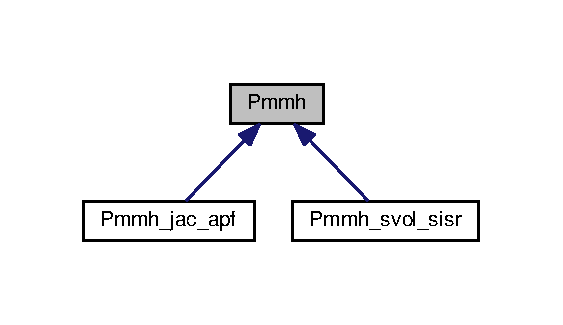
\includegraphics[width=270pt]{classPmmh__inherit__graph}
\end{center}
\end{figure}
\subsection*{Public Member Functions}
\begin{DoxyCompactItemize}
\item 
\hyperlink{classPmmh_aa4752fceaa1b278fcadb583865bfd0b5}{Pmmh} (const std\+::vector$<$ \hyperlink{pmfs_8h_a4c7df05c6f5e8a0d15ae14bcdbc07152}{Vec} $>$ \&start\+Theta, unsigned num\+M\+C\+M\+C\+Iters, const std\+::string \&data\+File, unsigned num\+Cols, bool mc)
\begin{DoxyCompactList}\small\item\em The constructor. \end{DoxyCompactList}\item 
\hyperlink{classPmmh_a52b058761ac6ede77eb3d8c0099e0d93}{$\sim$\+Pmmh} ()\hypertarget{classPmmh_a52b058761ac6ede77eb3d8c0099e0d93}{}\label{classPmmh_a52b058761ac6ede77eb3d8c0099e0d93}

\begin{DoxyCompactList}\small\item\em The destructor. \end{DoxyCompactList}\item 
void \hyperlink{classPmmh_ac035560cb209fb5cade23e431b5e1fd3}{commence\+Sampling} (std\+::string samples\+File, std\+::string messages\+File)
\begin{DoxyCompactList}\small\item\em Call this to begin sampling. \end{DoxyCompactList}\item 
virtual void \hyperlink{classPmmh_a7ada4decd5df894376c74e3ddba5daa1}{q\+Sample} (const std\+::vector$<$ \hyperlink{pmfs_8h_a4c7df05c6f5e8a0d15ae14bcdbc07152}{Vec} $>$ \&old\+Params, std\+::vector$<$ \hyperlink{pmfs_8h_a4c7df05c6f5e8a0d15ae14bcdbc07152}{Vec} $>$ \&new\+Params)=0
\begin{DoxyCompactList}\small\item\em The function that proposes new parameters. Tip\+: Make sure to declare your static R\+NG inside the implementation of this. \end{DoxyCompactList}\item 
virtual double \hyperlink{classPmmh_af8d3fdbc3f3c998670266a3032a53e80}{log\+Q\+Evaluate} (const std\+::vector$<$ \hyperlink{pmfs_8h_a4c7df05c6f5e8a0d15ae14bcdbc07152}{Vec} $>$ \&old\+Params, const std\+::vector$<$ \hyperlink{pmfs_8h_a4c7df05c6f5e8a0d15ae14bcdbc07152}{Vec} $>$ \&new\+Params)=0
\begin{DoxyCompactList}\small\item\em Evaluates the logarithm of the proposal density. \end{DoxyCompactList}\item 
virtual double \hyperlink{classPmmh_a265ca1c1380d0ebc052be2c5424a0d3b}{log\+Prior\+Evaluate} (const std\+::vector$<$ \hyperlink{pmfs_8h_a4c7df05c6f5e8a0d15ae14bcdbc07152}{Vec} $>$ \&theta)=0
\begin{DoxyCompactList}\small\item\em Evaluates the log of the model\textquotesingle{}s prior distribution. \end{DoxyCompactList}\item 
virtual double \hyperlink{classPmmh_a293931e138576f063aab7e46228f0266}{log\+Like\+Evaluate} (const std\+::vector$<$ \hyperlink{pmfs_8h_a4c7df05c6f5e8a0d15ae14bcdbc07152}{Vec} $>$ \&theta, const std\+::vector$<$ \hyperlink{pmfs_8h_a4c7df05c6f5e8a0d15ae14bcdbc07152}{Vec} $>$ \&data, std\+::atomic\+\_\+bool \&cancelled)=0
\begin{DoxyCompactList}\small\item\em Evaluates (approximates) the log-\/likelihood with a particle filter. \end{DoxyCompactList}\end{DoxyCompactItemize}


\subsection{Detailed Description}
A base-\/class for particle marginal Metropolis-\/\+Hastings. 

\begin{DoxyAuthor}{Author}
taylor 
\end{DoxyAuthor}
\begin{DoxyDate}{Date}
10/14/17 
\end{DoxyDate}


\subsection{Constructor \& Destructor Documentation}
\index{Pmmh@{Pmmh}!Pmmh@{Pmmh}}
\index{Pmmh@{Pmmh}!Pmmh@{Pmmh}}
\subsubsection[{\texorpdfstring{Pmmh(const std\+::vector$<$ Vec $>$ \&start\+Theta, unsigned num\+M\+C\+M\+C\+Iters, const std\+::string \&data\+File, unsigned num\+Cols, bool mc)}{Pmmh(const std::vector< Vec > &startTheta, unsigned numMCMCIters, const std::string &dataFile, unsigned numCols, bool mc)}}]{\setlength{\rightskip}{0pt plus 5cm}Pmmh\+::\+Pmmh (
\begin{DoxyParamCaption}
\item[{const std\+::vector$<$ {\bf Vec} $>$ \&}]{start\+Theta, }
\item[{unsigned}]{num\+M\+C\+M\+C\+Iters, }
\item[{const std\+::string \&}]{data\+File, }
\item[{unsigned}]{num\+Cols, }
\item[{bool}]{mc}
\end{DoxyParamCaption}
)}\hypertarget{classPmmh_aa4752fceaa1b278fcadb583865bfd0b5}{}\label{classPmmh_aa4752fceaa1b278fcadb583865bfd0b5}


The constructor. 


\begin{DoxyParams}{Parameters}
{\em start\+Theta} & the initial parameters you want to start sampling from. \\
\hline
{\em num\+M\+C\+M\+C\+Iters} & the number of M\+C\+MC iterations you want to do. \\
\hline
{\em data\+File} & the location of the observed time series data. \\
\hline
{\em num\+Cols} & the dimension of your observable data. \\
\hline
{\em mc} & stands for multicore. true or false if you want to use extra cores. \\
\hline
\end{DoxyParams}


\subsection{Member Function Documentation}
\index{Pmmh@{Pmmh}!commence\+Sampling@{commence\+Sampling}}
\index{commence\+Sampling@{commence\+Sampling}!Pmmh@{Pmmh}}
\subsubsection[{\texorpdfstring{commence\+Sampling(std\+::string samples\+File, std\+::string messages\+File)}{commenceSampling(std::string samplesFile, std::string messagesFile)}}]{\setlength{\rightskip}{0pt plus 5cm}void Pmmh\+::commence\+Sampling (
\begin{DoxyParamCaption}
\item[{std\+::string}]{samples\+File, }
\item[{std\+::string}]{messages\+File}
\end{DoxyParamCaption}
)}\hypertarget{classPmmh_ac035560cb209fb5cade23e431b5e1fd3}{}\label{classPmmh_ac035560cb209fb5cade23e431b5e1fd3}


Call this to begin sampling. 


\begin{DoxyParams}{Parameters}
{\em samples\+File} & where to store the csv of parameter samples. \\
\hline
{\em messages\+File} & where to store the logged messages. \\
\hline
\end{DoxyParams}
\index{Pmmh@{Pmmh}!log\+Like\+Evaluate@{log\+Like\+Evaluate}}
\index{log\+Like\+Evaluate@{log\+Like\+Evaluate}!Pmmh@{Pmmh}}
\subsubsection[{\texorpdfstring{log\+Like\+Evaluate(const std\+::vector$<$ Vec $>$ \&theta, const std\+::vector$<$ Vec $>$ \&data, std\+::atomic\+\_\+bool \&cancelled)=0}{logLikeEvaluate(const std::vector< Vec > &theta, const std::vector< Vec > &data, std::atomic_bool &cancelled)=0}}]{\setlength{\rightskip}{0pt plus 5cm}virtual double Pmmh\+::log\+Like\+Evaluate (
\begin{DoxyParamCaption}
\item[{const std\+::vector$<$ {\bf Vec} $>$ \&}]{theta, }
\item[{const std\+::vector$<$ {\bf Vec} $>$ \&}]{data, }
\item[{std\+::atomic\+\_\+bool \&}]{cancelled}
\end{DoxyParamCaption}
)\hspace{0.3cm}{\ttfamily [pure virtual]}}\hypertarget{classPmmh_a293931e138576f063aab7e46228f0266}{}\label{classPmmh_a293931e138576f063aab7e46228f0266}


Evaluates (approximates) the log-\/likelihood with a particle filter. 


\begin{DoxyParams}{Parameters}
{\em theta} & the parameters with which to run the particle filter. \\
\hline
{\em data} & the observed data with which to run the particle filter. \\
\hline
{\em cancelled} & is a token you need to provide if doing multithreaded likelihood evals. This allows the function to terminate prematurely. \\
\hline
\end{DoxyParams}
\begin{DoxyReturn}{Returns}
the evaluation (as a double) of the log likelihood approximation. 
\end{DoxyReturn}


Implemented in \hyperlink{classPmmh__svol__sisr_af0bb463ef4d74e60022a4955f565390e}{Pmmh\+\_\+svol\+\_\+sisr}, and \hyperlink{classPmmh__jac__apf_acd0869e2b01566fcd45d85e850d4ee11}{Pmmh\+\_\+jac\+\_\+apf}.

\index{Pmmh@{Pmmh}!log\+Prior\+Evaluate@{log\+Prior\+Evaluate}}
\index{log\+Prior\+Evaluate@{log\+Prior\+Evaluate}!Pmmh@{Pmmh}}
\subsubsection[{\texorpdfstring{log\+Prior\+Evaluate(const std\+::vector$<$ Vec $>$ \&theta)=0}{logPriorEvaluate(const std::vector< Vec > &theta)=0}}]{\setlength{\rightskip}{0pt plus 5cm}virtual double Pmmh\+::log\+Prior\+Evaluate (
\begin{DoxyParamCaption}
\item[{const std\+::vector$<$ {\bf Vec} $>$ \&}]{theta}
\end{DoxyParamCaption}
)\hspace{0.3cm}{\ttfamily [pure virtual]}}\hypertarget{classPmmh_a265ca1c1380d0ebc052be2c5424a0d3b}{}\label{classPmmh_a265ca1c1380d0ebc052be2c5424a0d3b}


Evaluates the log of the model\textquotesingle{}s prior distribution. 


\begin{DoxyParams}{Parameters}
{\em theta} & the parameters argument. \\
\hline
\end{DoxyParams}
\begin{DoxyReturn}{Returns}
the log of the prior density. 
\end{DoxyReturn}


Implemented in \hyperlink{classPmmh__svol__sisr_ab6c9983faf8ca460f8a8081c6a148aa2}{Pmmh\+\_\+svol\+\_\+sisr}, and \hyperlink{classPmmh__jac__apf_ab253d4b6c59a5e9529d042eb7b98dc8a}{Pmmh\+\_\+jac\+\_\+apf}.

\index{Pmmh@{Pmmh}!log\+Q\+Evaluate@{log\+Q\+Evaluate}}
\index{log\+Q\+Evaluate@{log\+Q\+Evaluate}!Pmmh@{Pmmh}}
\subsubsection[{\texorpdfstring{log\+Q\+Evaluate(const std\+::vector$<$ Vec $>$ \&old\+Params, const std\+::vector$<$ Vec $>$ \&new\+Params)=0}{logQEvaluate(const std::vector< Vec > &oldParams, const std::vector< Vec > &newParams)=0}}]{\setlength{\rightskip}{0pt plus 5cm}virtual double Pmmh\+::log\+Q\+Evaluate (
\begin{DoxyParamCaption}
\item[{const std\+::vector$<$ {\bf Vec} $>$ \&}]{old\+Params, }
\item[{const std\+::vector$<$ {\bf Vec} $>$ \&}]{new\+Params}
\end{DoxyParamCaption}
)\hspace{0.3cm}{\ttfamily [pure virtual]}}\hypertarget{classPmmh_af8d3fdbc3f3c998670266a3032a53e80}{}\label{classPmmh_af8d3fdbc3f3c998670266a3032a53e80}


Evaluates the logarithm of the proposal density. 


\begin{DoxyParams}{Parameters}
{\em old\+Params} & the old parameters. \\
\hline
{\em new\+Params} & the new parameters. \\
\hline
\end{DoxyParams}
\begin{DoxyReturn}{Returns}
the log of the proposal density. 
\end{DoxyReturn}


Implemented in \hyperlink{classPmmh__svol__sisr_a8164b385edb083df605ba766e000c12a}{Pmmh\+\_\+svol\+\_\+sisr}, and \hyperlink{classPmmh__jac__apf_a17edc1dc687fb753eff22d5bb7e44964}{Pmmh\+\_\+jac\+\_\+apf}.

\index{Pmmh@{Pmmh}!q\+Sample@{q\+Sample}}
\index{q\+Sample@{q\+Sample}!Pmmh@{Pmmh}}
\subsubsection[{\texorpdfstring{q\+Sample(const std\+::vector$<$ Vec $>$ \&old\+Params, std\+::vector$<$ Vec $>$ \&new\+Params)=0}{qSample(const std::vector< Vec > &oldParams, std::vector< Vec > &newParams)=0}}]{\setlength{\rightskip}{0pt plus 5cm}virtual void Pmmh\+::q\+Sample (
\begin{DoxyParamCaption}
\item[{const std\+::vector$<$ {\bf Vec} $>$ \&}]{old\+Params, }
\item[{std\+::vector$<$ {\bf Vec} $>$ \&}]{new\+Params}
\end{DoxyParamCaption}
)\hspace{0.3cm}{\ttfamily [pure virtual]}}\hypertarget{classPmmh_a7ada4decd5df894376c74e3ddba5daa1}{}\label{classPmmh_a7ada4decd5df894376c74e3ddba5daa1}


The function that proposes new parameters. Tip\+: Make sure to declare your static R\+NG inside the implementation of this. 


\begin{DoxyParams}{Parameters}
{\em old\+Params} & \\
\hline
{\em new\+Params} & \\
\hline
\end{DoxyParams}


Implemented in \hyperlink{classPmmh__svol__sisr_a18df26cb5c0bddefbd24866b1b4ff142}{Pmmh\+\_\+svol\+\_\+sisr}, and \hyperlink{classPmmh__jac__apf_a0127e07b0f9ba6b042418c575b78ca55}{Pmmh\+\_\+jac\+\_\+apf}.



The documentation for this class was generated from the following file\+:\begin{DoxyCompactItemize}
\item 
include/pmmh.\+h\end{DoxyCompactItemize}

\hypertarget{classSISRFilter}{}\section{S\+I\+S\+R\+Filter Class Reference}
\label{classSISRFilter}\index{S\+I\+S\+R\+Filter@{S\+I\+S\+R\+Filter}}


A base-\/class for Sequential Importance Sampling with Resampling.  




{\ttfamily \#include $<$sisr\+\_\+filter.\+h$>$}



Inheritance diagram for S\+I\+S\+R\+Filter\+:\nopagebreak
\begin{figure}[H]
\begin{center}
\leavevmode
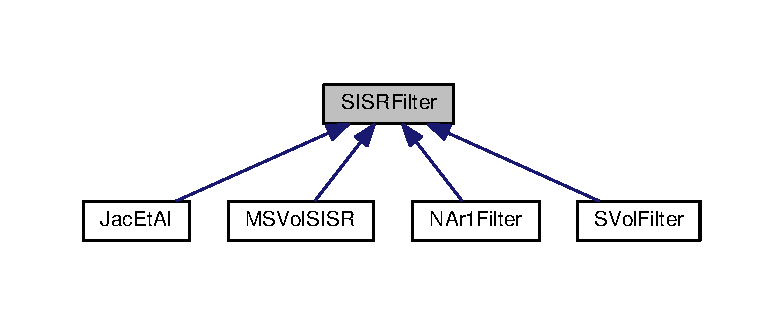
\includegraphics[width=350pt]{classSISRFilter__inherit__graph}
\end{center}
\end{figure}
\subsection*{Public Member Functions}
\begin{DoxyCompactItemize}
\item 
\hyperlink{classSISRFilter_a3105536db67f9aef8a08c32866a81a38}{S\+I\+S\+R\+Filter} (int num\+Parts, S\+I\+S\+R\+Resamp\+Style resamp\+Technique=S\+I\+S\+R\+Resamp\+Style\+::everytime\+\_\+multinomial, unsigned int path\+Length=0, double ess\+Perc=1.\+0)
\begin{DoxyCompactList}\small\item\em Constructor. \end{DoxyCompactList}\item 
\hyperlink{classSISRFilter_a6953590c7317c8dbf2341640dea71af8}{$\sim$\+S\+I\+S\+R\+Filter} ()\hypertarget{classSISRFilter_a6953590c7317c8dbf2341640dea71af8}{}\label{classSISRFilter_a6953590c7317c8dbf2341640dea71af8}

\begin{DoxyCompactList}\small\item\em Destructor. \end{DoxyCompactList}\item 
double \hyperlink{classSISRFilter_a9bec319e692266cacdd7e6cd9b60e77d}{get\+Log\+Cond\+Like} () const 
\begin{DoxyCompactList}\small\item\em get log p(y\+\_\+t$\vert$y\+\_\+\{1\+:t-\/1\})\$ or log p(y\+\_\+1). \end{DoxyCompactList}\item 
double \hyperlink{classSISRFilter_aab226ed51d07c493151a6788e6f90b86}{get\+E\+SS} () const 
\begin{DoxyCompactList}\small\item\em get effective sample size. \end{DoxyCompactList}\item 
std\+::vector$<$ std\+::vector$<$ \hyperlink{pmfs_8h_a4c7df05c6f5e8a0d15ae14bcdbc07152}{Vec} $>$ $>$ \hyperlink{classSISRFilter_a8ca159b052883c9c4dc0231145f6fe85}{get\+Full\+Parts} () const 
\begin{DoxyCompactList}\small\item\em get \$p(x\+\_\+\{1\+:t\}$\vert$y\+\_\+\{1\+:t\})\$ \end{DoxyCompactList}\item 
std\+::vector$<$ \hyperlink{pmfs_8h_ae601f56a556993079f730483c574356f}{Mat} $>$ \hyperlink{classSISRFilter_a4dd3b90b857114e599a8f71703cb768e}{get\+Expectations} () const 
\begin{DoxyCompactList}\small\item\em get all stored expectations. With respect to \$p(x\+\_\+t$\vert$y\+\_\+\{1\+:t\})\$ \end{DoxyCompactList}\item 
std\+::vector$<$ double $>$ \hyperlink{classSISRFilter_aa87ac349cbc21f70fb51c24fcbbc521a}{get\+Log\+U\+Weights} () const 
\begin{DoxyCompactList}\small\item\em Get log-\/un-\/normalized weights. \end{DoxyCompactList}\item 
void \hyperlink{classSISRFilter_a8c22a038dc47490b5532f2ec6c21a548}{filter\+Or\+Smooth} (const \hyperlink{pmfs_8h_a4c7df05c6f5e8a0d15ae14bcdbc07152}{Vec} \&data, const std\+::vector$<$ std\+::function$<$ const \hyperlink{pmfs_8h_ae601f56a556993079f730483c574356f}{Mat}(const \hyperlink{pmfs_8h_a4c7df05c6f5e8a0d15ae14bcdbc07152}{Vec} \&)$>$ $>$ \&fs=std\+::vector$<$ std\+::function$<$ const \hyperlink{pmfs_8h_ae601f56a556993079f730483c574356f}{Mat}(const \hyperlink{pmfs_8h_a4c7df05c6f5e8a0d15ae14bcdbc07152}{Vec} \&)$>$ $>$())
\begin{DoxyCompactList}\small\item\em If storing whole paths, performs smoothing. If not storing whole paths, performs filtering. \end{DoxyCompactList}\item 
virtual double \hyperlink{classSISRFilter_ab6ffa8e1cdee34f1afb825e35462afaa}{log\+Mu\+Ev} (const \hyperlink{pmfs_8h_a4c7df05c6f5e8a0d15ae14bcdbc07152}{Vec} \&x1)=0
\begin{DoxyCompactList}\small\item\em Calculate mu\+Ev or logmu\+Ev. \end{DoxyCompactList}\item 
virtual \hyperlink{pmfs_8h_a4c7df05c6f5e8a0d15ae14bcdbc07152}{Vec} \hyperlink{classSISRFilter_a5a57cd67535e31bb1ab20fb42499f911}{q1\+Samp} (const \hyperlink{pmfs_8h_a4c7df05c6f5e8a0d15ae14bcdbc07152}{Vec} \&y1)=0
\begin{DoxyCompactList}\small\item\em Samples from time 1 proposal. \end{DoxyCompactList}\item 
virtual double \hyperlink{classSISRFilter_a61a1971bd8208abbe3ccbacd66d35c23}{log\+Q1\+Ev} (const \hyperlink{pmfs_8h_a4c7df05c6f5e8a0d15ae14bcdbc07152}{Vec} \&x1, const \hyperlink{pmfs_8h_a4c7df05c6f5e8a0d15ae14bcdbc07152}{Vec} \&y1)=0
\begin{DoxyCompactList}\small\item\em Calculate q1\+Ev or log q1\+Ev. \end{DoxyCompactList}\item 
virtual double \hyperlink{classSISRFilter_aac59b077648fa74d2a5db970e3d7ffac}{log\+G\+Ev} (const \hyperlink{pmfs_8h_a4c7df05c6f5e8a0d15ae14bcdbc07152}{Vec} \&yt, const \hyperlink{pmfs_8h_a4c7df05c6f5e8a0d15ae14bcdbc07152}{Vec} \&xt)=0
\begin{DoxyCompactList}\small\item\em Calculate g\+Ev or log\+G\+Ev. \end{DoxyCompactList}\item 
virtual double \hyperlink{classSISRFilter_ab91474fc79efb84ed1dafbc8c542f59e}{log\+F\+Ev} (const \hyperlink{pmfs_8h_a4c7df05c6f5e8a0d15ae14bcdbc07152}{Vec} \&xt, const \hyperlink{pmfs_8h_a4c7df05c6f5e8a0d15ae14bcdbc07152}{Vec} \&xtm1)=0
\begin{DoxyCompactList}\small\item\em Calculate f\+Ev or log\+F\+Ev. \end{DoxyCompactList}\item 
virtual \hyperlink{pmfs_8h_a4c7df05c6f5e8a0d15ae14bcdbc07152}{Vec} \hyperlink{classSISRFilter_a2c480a10cac8b52a36ab1309cf9ea1a4}{q\+Samp} (const \hyperlink{pmfs_8h_a4c7df05c6f5e8a0d15ae14bcdbc07152}{Vec} \&xtm1, const \hyperlink{pmfs_8h_a4c7df05c6f5e8a0d15ae14bcdbc07152}{Vec} \&yt)=0
\begin{DoxyCompactList}\small\item\em Sample from the proposal distribution. \end{DoxyCompactList}\item 
virtual double \hyperlink{classSISRFilter_af289db59b008a0ab795fc3b8e9887043}{log\+Q\+Ev} (const \hyperlink{pmfs_8h_a4c7df05c6f5e8a0d15ae14bcdbc07152}{Vec} \&xt, const \hyperlink{pmfs_8h_a4c7df05c6f5e8a0d15ae14bcdbc07152}{Vec} \&xtm1, const \hyperlink{pmfs_8h_a4c7df05c6f5e8a0d15ae14bcdbc07152}{Vec} \&yt)=0
\begin{DoxyCompactList}\small\item\em Calculate q\+Ev or log\+Q\+Ev. \end{DoxyCompactList}\end{DoxyCompactItemize}


\subsection{Detailed Description}
A base-\/class for Sequential Importance Sampling with Resampling. 

\begin{DoxyAuthor}{Author}
taylor 
\end{DoxyAuthor}
\begin{DoxyDate}{Date}
07/09/17 
\end{DoxyDate}


\subsection{Constructor \& Destructor Documentation}
\index{S\+I\+S\+R\+Filter@{S\+I\+S\+R\+Filter}!S\+I\+S\+R\+Filter@{S\+I\+S\+R\+Filter}}
\index{S\+I\+S\+R\+Filter@{S\+I\+S\+R\+Filter}!S\+I\+S\+R\+Filter@{S\+I\+S\+R\+Filter}}
\subsubsection[{\texorpdfstring{S\+I\+S\+R\+Filter(int num\+Parts, S\+I\+S\+R\+Resamp\+Style resamp\+Technique=\+S\+I\+S\+R\+Resamp\+Style\+::everytime\+\_\+multinomial, unsigned int path\+Length=0, double ess\+Perc=1.\+0)}{SISRFilter(int numParts, SISRResampStyle resampTechnique=SISRResampStyle::everytime_multinomial, unsigned int pathLength=0, double essPerc=1.0)}}]{\setlength{\rightskip}{0pt plus 5cm}S\+I\+S\+R\+Filter\+::\+S\+I\+S\+R\+Filter (
\begin{DoxyParamCaption}
\item[{int}]{num\+Parts, }
\item[{S\+I\+S\+R\+Resamp\+Style}]{resamp\+Technique = {\ttfamily SISRResampStyle\+:\+:everytime\+\_\+multinomial}, }
\item[{unsigned int}]{path\+Length = {\ttfamily 0}, }
\item[{double}]{ess\+Perc = {\ttfamily 1.0}}
\end{DoxyParamCaption}
)}\hypertarget{classSISRFilter_a3105536db67f9aef8a08c32866a81a38}{}\label{classSISRFilter_a3105536db67f9aef8a08c32866a81a38}


Constructor. 


\begin{DoxyParams}{Parameters}
{\em num\+Parts} & number of particles \\
\hline
{\em resamp\+Technique} & which resampling strategy? \\
\hline
{\em path\+Length} & Set to 0 if you don\textquotesingle{}t want save entire paths. Otherwise, enter time length. \\
\hline
{\em ess\+Perc} & ignored unless S\+I\+S\+R\+Resamp\+Style is \char`\"{}ess.\char`\"{} What percent of E\+SS is the threshold for resampling. \\
\hline
\end{DoxyParams}


\subsection{Member Function Documentation}
\index{S\+I\+S\+R\+Filter@{S\+I\+S\+R\+Filter}!filter\+Or\+Smooth@{filter\+Or\+Smooth}}
\index{filter\+Or\+Smooth@{filter\+Or\+Smooth}!S\+I\+S\+R\+Filter@{S\+I\+S\+R\+Filter}}
\subsubsection[{\texorpdfstring{filter\+Or\+Smooth(const Vec \&data, const std\+::vector$<$ std\+::function$<$ const Mat(const Vec \&)$>$ $>$ \&fs=std\+::vector$<$ std\+::function$<$ const Mat(const Vec \&)$>$ $>$())}{filterOrSmooth(const Vec &data, const std::vector< std::function< const Mat(const Vec &)> > &fs=std::vector< std::function< const Mat(const Vec &)> >())}}]{\setlength{\rightskip}{0pt plus 5cm}void S\+I\+S\+R\+Filter\+::filter\+Or\+Smooth (
\begin{DoxyParamCaption}
\item[{const {\bf Vec} \&}]{data, }
\item[{const std\+::vector$<$ std\+::function$<$ const {\bf Mat}(const {\bf Vec} \&)$>$ $>$ \&}]{fs = {\ttfamily std\+:\+:vector$<$~std\+:\+:function$<$~const~{\bf Mat}(const~{\bf Vec}~\&)$>$~$>$()}}
\end{DoxyParamCaption}
)}\hypertarget{classSISRFilter_a8c22a038dc47490b5532f2ec6c21a548}{}\label{classSISRFilter_a8c22a038dc47490b5532f2ec6c21a548}


If storing whole paths, performs smoothing. If not storing whole paths, performs filtering. 


\begin{DoxyParams}{Parameters}
{\em data} & is a const Vec\& representing the current observed value of the time series. \\
\hline
{\em fs} & is a vector of functions that operate on each particle Vec. They are used to store empirical expectations (taken with respect to the filtering distribution). \\
\hline
\end{DoxyParams}
\index{S\+I\+S\+R\+Filter@{S\+I\+S\+R\+Filter}!get\+E\+SS@{get\+E\+SS}}
\index{get\+E\+SS@{get\+E\+SS}!S\+I\+S\+R\+Filter@{S\+I\+S\+R\+Filter}}
\subsubsection[{\texorpdfstring{get\+E\+S\+S() const }{getESS() const }}]{\setlength{\rightskip}{0pt plus 5cm}double S\+I\+S\+R\+Filter\+::get\+E\+SS (
\begin{DoxyParamCaption}
{}
\end{DoxyParamCaption}
) const}\hypertarget{classSISRFilter_aab226ed51d07c493151a6788e6f90b86}{}\label{classSISRFilter_aab226ed51d07c493151a6788e6f90b86}


get effective sample size. 

\begin{DoxyReturn}{Returns}
The current estimate for the effective sample size. 
\end{DoxyReturn}
\index{S\+I\+S\+R\+Filter@{S\+I\+S\+R\+Filter}!get\+Expectations@{get\+Expectations}}
\index{get\+Expectations@{get\+Expectations}!S\+I\+S\+R\+Filter@{S\+I\+S\+R\+Filter}}
\subsubsection[{\texorpdfstring{get\+Expectations() const }{getExpectations() const }}]{\setlength{\rightskip}{0pt plus 5cm}std\+::vector$<${\bf Mat}$>$ S\+I\+S\+R\+Filter\+::get\+Expectations (
\begin{DoxyParamCaption}
{}
\end{DoxyParamCaption}
) const}\hypertarget{classSISRFilter_a4dd3b90b857114e599a8f71703cb768e}{}\label{classSISRFilter_a4dd3b90b857114e599a8f71703cb768e}


get all stored expectations. With respect to \$p(x\+\_\+t$\vert$y\+\_\+\{1\+:t\})\$ 

\begin{DoxyReturn}{Returns}
returns a std\+::vector$<$\+Mat$>$ of all of the approximated expectations. 
\end{DoxyReturn}
\index{S\+I\+S\+R\+Filter@{S\+I\+S\+R\+Filter}!get\+Full\+Parts@{get\+Full\+Parts}}
\index{get\+Full\+Parts@{get\+Full\+Parts}!S\+I\+S\+R\+Filter@{S\+I\+S\+R\+Filter}}
\subsubsection[{\texorpdfstring{get\+Full\+Parts() const }{getFullParts() const }}]{\setlength{\rightskip}{0pt plus 5cm}std\+::vector$<$std\+::vector$<${\bf Vec}$>$ $>$ S\+I\+S\+R\+Filter\+::get\+Full\+Parts (
\begin{DoxyParamCaption}
{}
\end{DoxyParamCaption}
) const}\hypertarget{classSISRFilter_a8ca159b052883c9c4dc0231145f6fe85}{}\label{classSISRFilter_a8ca159b052883c9c4dc0231145f6fe85}


get \$p(x\+\_\+\{1\+:t\}$\vert$y\+\_\+\{1\+:t\})\$ 

\begin{DoxyReturn}{Returns}
The up-\/to-\/date set of path samples for the joint smoothing distribution. 
\end{DoxyReturn}
\index{S\+I\+S\+R\+Filter@{S\+I\+S\+R\+Filter}!get\+Log\+Cond\+Like@{get\+Log\+Cond\+Like}}
\index{get\+Log\+Cond\+Like@{get\+Log\+Cond\+Like}!S\+I\+S\+R\+Filter@{S\+I\+S\+R\+Filter}}
\subsubsection[{\texorpdfstring{get\+Log\+Cond\+Like() const }{getLogCondLike() const }}]{\setlength{\rightskip}{0pt plus 5cm}double S\+I\+S\+R\+Filter\+::get\+Log\+Cond\+Like (
\begin{DoxyParamCaption}
{}
\end{DoxyParamCaption}
) const}\hypertarget{classSISRFilter_a9bec319e692266cacdd7e6cd9b60e77d}{}\label{classSISRFilter_a9bec319e692266cacdd7e6cd9b60e77d}


get log p(y\+\_\+t$\vert$y\+\_\+\{1\+:t-\/1\})\$ or log p(y\+\_\+1). 

\begin{DoxyReturn}{Returns}
The estimate of the most recent log conditional likelihood. 
\end{DoxyReturn}
\index{S\+I\+S\+R\+Filter@{S\+I\+S\+R\+Filter}!get\+Log\+U\+Weights@{get\+Log\+U\+Weights}}
\index{get\+Log\+U\+Weights@{get\+Log\+U\+Weights}!S\+I\+S\+R\+Filter@{S\+I\+S\+R\+Filter}}
\subsubsection[{\texorpdfstring{get\+Log\+U\+Weights() const }{getLogUWeights() const }}]{\setlength{\rightskip}{0pt plus 5cm}std\+::vector$<$double$>$ S\+I\+S\+R\+Filter\+::get\+Log\+U\+Weights (
\begin{DoxyParamCaption}
{}
\end{DoxyParamCaption}
) const}\hypertarget{classSISRFilter_aa87ac349cbc21f70fb51c24fcbbc521a}{}\label{classSISRFilter_aa87ac349cbc21f70fb51c24fcbbc521a}


Get log-\/un-\/normalized weights. 

\begin{DoxyReturn}{Returns}
The most recent std\+::vector of log-\/un-\/normalized weights. 
\end{DoxyReturn}
\index{S\+I\+S\+R\+Filter@{S\+I\+S\+R\+Filter}!log\+F\+Ev@{log\+F\+Ev}}
\index{log\+F\+Ev@{log\+F\+Ev}!S\+I\+S\+R\+Filter@{S\+I\+S\+R\+Filter}}
\subsubsection[{\texorpdfstring{log\+F\+Ev(const Vec \&xt, const Vec \&xtm1)=0}{logFEv(const Vec &xt, const Vec &xtm1)=0}}]{\setlength{\rightskip}{0pt plus 5cm}virtual double S\+I\+S\+R\+Filter\+::log\+F\+Ev (
\begin{DoxyParamCaption}
\item[{const {\bf Vec} \&}]{xt, }
\item[{const {\bf Vec} \&}]{xtm1}
\end{DoxyParamCaption}
)\hspace{0.3cm}{\ttfamily [pure virtual]}}\hypertarget{classSISRFilter_ab91474fc79efb84ed1dafbc8c542f59e}{}\label{classSISRFilter_ab91474fc79efb84ed1dafbc8c542f59e}


Calculate f\+Ev or log\+F\+Ev. 


\begin{DoxyParams}{Parameters}
{\em xt} & is a const Vec\& describing the time t state \\
\hline
{\em xtm1} & is a const Vec\& describing the time t-\/1 state \\
\hline
\end{DoxyParams}
\begin{DoxyReturn}{Returns}
the density or log-\/denity evaluation as a double 
\end{DoxyReturn}


Implemented in \hyperlink{classNAr1Filter_adff7d17aa5271b8df4c77d752a6fd773}{N\+Ar1\+Filter}, \hyperlink{classJacEtAl_a7742c736cf4136968dcf8629c4a3914e}{Jac\+Et\+Al}, \hyperlink{classMSVolSISR_acd51af2d17300973b8fa4748e5729f3c}{M\+S\+Vol\+S\+I\+SR}, and \hyperlink{classSVolFilter_a506d813662f0d888e48607962bfefbbd}{S\+Vol\+Filter}.

\index{S\+I\+S\+R\+Filter@{S\+I\+S\+R\+Filter}!log\+G\+Ev@{log\+G\+Ev}}
\index{log\+G\+Ev@{log\+G\+Ev}!S\+I\+S\+R\+Filter@{S\+I\+S\+R\+Filter}}
\subsubsection[{\texorpdfstring{log\+G\+Ev(const Vec \&yt, const Vec \&xt)=0}{logGEv(const Vec &yt, const Vec &xt)=0}}]{\setlength{\rightskip}{0pt plus 5cm}virtual double S\+I\+S\+R\+Filter\+::log\+G\+Ev (
\begin{DoxyParamCaption}
\item[{const {\bf Vec} \&}]{yt, }
\item[{const {\bf Vec} \&}]{xt}
\end{DoxyParamCaption}
)\hspace{0.3cm}{\ttfamily [pure virtual]}}\hypertarget{classSISRFilter_aac59b077648fa74d2a5db970e3d7ffac}{}\label{classSISRFilter_aac59b077648fa74d2a5db970e3d7ffac}


Calculate g\+Ev or log\+G\+Ev. 


\begin{DoxyParams}{Parameters}
{\em yt} & is a const Vec\& describing the time t datum \\
\hline
{\em xt} & is a const Vec\& describing the time t state \\
\hline
\end{DoxyParams}
\begin{DoxyReturn}{Returns}
the density or log-\/density evaluation as a double 
\end{DoxyReturn}


Implemented in \hyperlink{classNAr1Filter_aed4a7fb8160aabe9a7dc702826ccae60}{N\+Ar1\+Filter}, \hyperlink{classJacEtAl_aa37b7701fac288d76b72640b2c98f253}{Jac\+Et\+Al}, \hyperlink{classMSVolSISR_a1e7efc4dd05351872764983a99a0c5ed}{M\+S\+Vol\+S\+I\+SR}, and \hyperlink{classSVolFilter_a81a8e2857ddb699738461b5e2beab1c0}{S\+Vol\+Filter}.

\index{S\+I\+S\+R\+Filter@{S\+I\+S\+R\+Filter}!log\+Mu\+Ev@{log\+Mu\+Ev}}
\index{log\+Mu\+Ev@{log\+Mu\+Ev}!S\+I\+S\+R\+Filter@{S\+I\+S\+R\+Filter}}
\subsubsection[{\texorpdfstring{log\+Mu\+Ev(const Vec \&x1)=0}{logMuEv(const Vec &x1)=0}}]{\setlength{\rightskip}{0pt plus 5cm}virtual double S\+I\+S\+R\+Filter\+::log\+Mu\+Ev (
\begin{DoxyParamCaption}
\item[{const {\bf Vec} \&}]{x1}
\end{DoxyParamCaption}
)\hspace{0.3cm}{\ttfamily [pure virtual]}}\hypertarget{classSISRFilter_ab6ffa8e1cdee34f1afb825e35462afaa}{}\label{classSISRFilter_ab6ffa8e1cdee34f1afb825e35462afaa}


Calculate mu\+Ev or logmu\+Ev. 


\begin{DoxyParams}{Parameters}
{\em x1} & is a const Vec\& describing the state sample \\
\hline
\end{DoxyParams}
\begin{DoxyReturn}{Returns}
the density or log-\/density evaluation as a double 
\end{DoxyReturn}


Implemented in \hyperlink{classNAr1Filter_ac97b366af3d4def2b45d394fb85865f0}{N\+Ar1\+Filter}, \hyperlink{classJacEtAl_a96f970a2b0e7f0583a5fe567b6353ffe}{Jac\+Et\+Al}, \hyperlink{classMSVolSISR_a2af842b09bada27765bf8e7e60c59183}{M\+S\+Vol\+S\+I\+SR}, and \hyperlink{classSVolFilter_ab052dcfa9ce2100ffb02350ccf0b6d17}{S\+Vol\+Filter}.

\index{S\+I\+S\+R\+Filter@{S\+I\+S\+R\+Filter}!log\+Q1\+Ev@{log\+Q1\+Ev}}
\index{log\+Q1\+Ev@{log\+Q1\+Ev}!S\+I\+S\+R\+Filter@{S\+I\+S\+R\+Filter}}
\subsubsection[{\texorpdfstring{log\+Q1\+Ev(const Vec \&x1, const Vec \&y1)=0}{logQ1Ev(const Vec &x1, const Vec &y1)=0}}]{\setlength{\rightskip}{0pt plus 5cm}virtual double S\+I\+S\+R\+Filter\+::log\+Q1\+Ev (
\begin{DoxyParamCaption}
\item[{const {\bf Vec} \&}]{x1, }
\item[{const {\bf Vec} \&}]{y1}
\end{DoxyParamCaption}
)\hspace{0.3cm}{\ttfamily [pure virtual]}}\hypertarget{classSISRFilter_a61a1971bd8208abbe3ccbacd66d35c23}{}\label{classSISRFilter_a61a1971bd8208abbe3ccbacd66d35c23}


Calculate q1\+Ev or log q1\+Ev. 


\begin{DoxyParams}{Parameters}
{\em x1} & is a const Vec\& describing the time 1 state sample \\
\hline
{\em y1} & is a const Vec\& describing the time 1 datum \\
\hline
\end{DoxyParams}
\begin{DoxyReturn}{Returns}
the density or log-\/density evaluation as a double 
\end{DoxyReturn}


Implemented in \hyperlink{classNAr1Filter_af8eb2b66ff1806dd0d4c4ac1f7129a51}{N\+Ar1\+Filter}, \hyperlink{classJacEtAl_aec5fff50e30a9df174b04f2ab53c73d0}{Jac\+Et\+Al}, \hyperlink{classMSVolSISR_a9c776bfbf157ff4f0dc3cbe1c4212142}{M\+S\+Vol\+S\+I\+SR}, and \hyperlink{classSVolFilter_a9adc1eb288e46a2e05fa89d1b8d9f1ef}{S\+Vol\+Filter}.

\index{S\+I\+S\+R\+Filter@{S\+I\+S\+R\+Filter}!log\+Q\+Ev@{log\+Q\+Ev}}
\index{log\+Q\+Ev@{log\+Q\+Ev}!S\+I\+S\+R\+Filter@{S\+I\+S\+R\+Filter}}
\subsubsection[{\texorpdfstring{log\+Q\+Ev(const Vec \&xt, const Vec \&xtm1, const Vec \&yt)=0}{logQEv(const Vec &xt, const Vec &xtm1, const Vec &yt)=0}}]{\setlength{\rightskip}{0pt plus 5cm}virtual double S\+I\+S\+R\+Filter\+::log\+Q\+Ev (
\begin{DoxyParamCaption}
\item[{const {\bf Vec} \&}]{xt, }
\item[{const {\bf Vec} \&}]{xtm1, }
\item[{const {\bf Vec} \&}]{yt}
\end{DoxyParamCaption}
)\hspace{0.3cm}{\ttfamily [pure virtual]}}\hypertarget{classSISRFilter_af289db59b008a0ab795fc3b8e9887043}{}\label{classSISRFilter_af289db59b008a0ab795fc3b8e9887043}


Calculate q\+Ev or log\+Q\+Ev. 


\begin{DoxyParams}{Parameters}
{\em xt} & is a const Vec\& describing the time t state \\
\hline
{\em xtm1} & is a const Vec\& describing the time t-\/1 state \\
\hline
{\em yt} & is a const Vec\& describing the time t datum \\
\hline
\end{DoxyParams}
\begin{DoxyReturn}{Returns}
the density or log-\/density evaluation as a double 
\end{DoxyReturn}


Implemented in \hyperlink{classNAr1Filter_ae42e9ccf333b8590bd79831be8083dcd}{N\+Ar1\+Filter}, \hyperlink{classJacEtAl_a73a94bbb16389102b20def8c0bdf96d8}{Jac\+Et\+Al}, \hyperlink{classMSVolSISR_af5ef1c3d5499bc9f2693a3f918def613}{M\+S\+Vol\+S\+I\+SR}, and \hyperlink{classSVolFilter_af2bbbe9c2d3bddb3e85b9ed5a14a24cb}{S\+Vol\+Filter}.

\index{S\+I\+S\+R\+Filter@{S\+I\+S\+R\+Filter}!q1\+Samp@{q1\+Samp}}
\index{q1\+Samp@{q1\+Samp}!S\+I\+S\+R\+Filter@{S\+I\+S\+R\+Filter}}
\subsubsection[{\texorpdfstring{q1\+Samp(const Vec \&y1)=0}{q1Samp(const Vec &y1)=0}}]{\setlength{\rightskip}{0pt plus 5cm}virtual {\bf Vec} S\+I\+S\+R\+Filter\+::q1\+Samp (
\begin{DoxyParamCaption}
\item[{const {\bf Vec} \&}]{y1}
\end{DoxyParamCaption}
)\hspace{0.3cm}{\ttfamily [pure virtual]}}\hypertarget{classSISRFilter_a5a57cd67535e31bb1ab20fb42499f911}{}\label{classSISRFilter_a5a57cd67535e31bb1ab20fb42499f911}


Samples from time 1 proposal. 


\begin{DoxyParams}{Parameters}
{\em y1} & is a const Vec\& representing the first observed datum \\
\hline
\end{DoxyParams}
\begin{DoxyReturn}{Returns}
the sample as a Vec 
\end{DoxyReturn}


Implemented in \hyperlink{classSVolFilter_aaea1d4b59cdd3053f060d5013e338162}{S\+Vol\+Filter}, \hyperlink{classNAr1Filter_a6ae702c69b4f3e7b2109f99e2fd5d8b7}{N\+Ar1\+Filter}, \hyperlink{classJacEtAl_a154ca22da5c981f2d0c9515dc89a472c}{Jac\+Et\+Al}, and \hyperlink{classMSVolSISR_ac828fdce8a00f9ac3adbe0fa019fe49d}{M\+S\+Vol\+S\+I\+SR}.

\index{S\+I\+S\+R\+Filter@{S\+I\+S\+R\+Filter}!q\+Samp@{q\+Samp}}
\index{q\+Samp@{q\+Samp}!S\+I\+S\+R\+Filter@{S\+I\+S\+R\+Filter}}
\subsubsection[{\texorpdfstring{q\+Samp(const Vec \&xtm1, const Vec \&yt)=0}{qSamp(const Vec &xtm1, const Vec &yt)=0}}]{\setlength{\rightskip}{0pt plus 5cm}virtual {\bf Vec} S\+I\+S\+R\+Filter\+::q\+Samp (
\begin{DoxyParamCaption}
\item[{const {\bf Vec} \&}]{xtm1, }
\item[{const {\bf Vec} \&}]{yt}
\end{DoxyParamCaption}
)\hspace{0.3cm}{\ttfamily [pure virtual]}}\hypertarget{classSISRFilter_a2c480a10cac8b52a36ab1309cf9ea1a4}{}\label{classSISRFilter_a2c480a10cac8b52a36ab1309cf9ea1a4}


Sample from the proposal distribution. 


\begin{DoxyParams}{Parameters}
{\em xtm1} & is a const Vec\& describing the time t-\/1 state \\
\hline
{\em yt} & is a const Vec\& describing the time t datum \\
\hline
\end{DoxyParams}
\begin{DoxyReturn}{Returns}
the sample as a Vec 
\end{DoxyReturn}


Implemented in \hyperlink{classNAr1Filter_af4f7f8b643e5750dc83e27ea7bf05f18}{N\+Ar1\+Filter}, \hyperlink{classJacEtAl_a2b2696527c89fdf462639e55dfbc67ce}{Jac\+Et\+Al}, \hyperlink{classMSVolSISR_a4f2f68902ba97f6dee582f1f01d1f5d7}{M\+S\+Vol\+S\+I\+SR}, and \hyperlink{classSVolFilter_a754e3c40b1db7798a48f3f4ad636b07c}{S\+Vol\+Filter}.



The documentation for this class was generated from the following file\+:\begin{DoxyCompactItemize}
\item 
include/sisr\+\_\+filter.\+h\end{DoxyCompactItemize}

\hypertarget{classSISRSmoother}{}\section{S\+I\+S\+R\+Smoother Class Reference}
\label{classSISRSmoother}\index{S\+I\+S\+R\+Smoother@{S\+I\+S\+R\+Smoother}}


A base-\/class for Sequential Importance Sampling with Resampling.  




{\ttfamily \#include $<$sisr\+\_\+smooth.\+h$>$}

\subsection*{Public Member Functions}
\begin{DoxyCompactItemize}
\item 
\hyperlink{classSISRSmoother_a1d2c23e5a42ad2529335126f8b5e744e}{S\+I\+S\+R\+Smoother} (int num\+Parts, \hyperlink{sisr__filter_8h_a2486051fd2028dedca520d3e0f8fd92f}{S\+I\+S\+R\+Resamp\+Style} resamp\+Technique=S\+I\+S\+R\+Resamp\+Style\+::everytime\+\_\+multinomial, unsigned int path\+Length=0, double ess\+Perc=1.\+0)
\begin{DoxyCompactList}\small\item\em Constructor. \end{DoxyCompactList}\item 
\hyperlink{classSISRSmoother_a800ef5dc1cda37c7f0f0fd7f70ac0696}{$\sim$\+S\+I\+S\+R\+Smoother} ()\hypertarget{classSISRSmoother_a800ef5dc1cda37c7f0f0fd7f70ac0696}{}\label{classSISRSmoother_a800ef5dc1cda37c7f0f0fd7f70ac0696}

\begin{DoxyCompactList}\small\item\em Destructor. \end{DoxyCompactList}\item 
double \hyperlink{classSISRSmoother_a6316bfec4e62d522e1fe32f8c4b18b0f}{get\+Log\+Cond\+Like} () const 
\begin{DoxyCompactList}\small\item\em get log p(y\+\_\+t$\vert$y\+\_\+\{1\+:t-\/1\})\$ or log p(y\+\_\+1). \end{DoxyCompactList}\item 
double \hyperlink{classSISRSmoother_a9e6a9e4681075c1ea28a7476b261e1fc}{get\+E\+SS} () const 
\begin{DoxyCompactList}\small\item\em get effective sample size. \end{DoxyCompactList}\item 
std\+::vector$<$ std\+::vector$<$ \hyperlink{apf__filter_8h_a4c7df05c6f5e8a0d15ae14bcdbc07152}{Vec} $>$ $>$ \hyperlink{classSISRSmoother_a52ba9c6f180491ed1751772bb832c5ac}{get\+Full\+Parts} () const 
\begin{DoxyCompactList}\small\item\em get \$p(x\+\_\+\{1\+:t\}$\vert$y\+\_\+\{1\+:t\})\$ \end{DoxyCompactList}\item 
std\+::vector$<$ double $>$ \hyperlink{classSISRSmoother_af7ede0870c83af1e4accfa70675b21bc}{get\+Log\+U\+Weights} () const 
\begin{DoxyCompactList}\small\item\em Get log-\/un-\/normalized weights. \end{DoxyCompactList}\item 
void \hyperlink{classSISRSmoother_a11193002ca13b8186167f7c3f6db625c}{smooth} (const \hyperlink{apf__filter_8h_a4c7df05c6f5e8a0d15ae14bcdbc07152}{Vec} \&data)
\begin{DoxyCompactList}\small\item\em If storing whole paths, performs smoothing. If not storing whole paths, performs filtering. \end{DoxyCompactList}\item 
virtual double \hyperlink{classSISRSmoother_a5498af2a7a572435f303a2238c252464}{log\+Mu\+Ev} (const \hyperlink{apf__filter_8h_a4c7df05c6f5e8a0d15ae14bcdbc07152}{Vec} \&x1)=0
\begin{DoxyCompactList}\small\item\em Calculate mu\+Ev or logmu\+Ev. \end{DoxyCompactList}\item 
virtual \hyperlink{apf__filter_8h_a4c7df05c6f5e8a0d15ae14bcdbc07152}{Vec} \hyperlink{classSISRSmoother_a1c7a32fa83f90fa6666bd0e739189275}{q1\+Samp} (const \hyperlink{apf__filter_8h_a4c7df05c6f5e8a0d15ae14bcdbc07152}{Vec} \&y1)=0
\begin{DoxyCompactList}\small\item\em Samples from time 1 proposal. \end{DoxyCompactList}\item 
virtual double \hyperlink{classSISRSmoother_a316ce1b0f0e18d277b0687f727a00a0a}{log\+Q1\+Ev} (const \hyperlink{apf__filter_8h_a4c7df05c6f5e8a0d15ae14bcdbc07152}{Vec} \&x1, const \hyperlink{apf__filter_8h_a4c7df05c6f5e8a0d15ae14bcdbc07152}{Vec} \&y1)=0
\begin{DoxyCompactList}\small\item\em Calculate q1\+Ev or log q1\+Ev. \end{DoxyCompactList}\item 
virtual double \hyperlink{classSISRSmoother_a15cafa515e345d7ea5b3afefcca27386}{log\+G\+Ev} (const \hyperlink{apf__filter_8h_a4c7df05c6f5e8a0d15ae14bcdbc07152}{Vec} \&yt, const \hyperlink{apf__filter_8h_a4c7df05c6f5e8a0d15ae14bcdbc07152}{Vec} \&xt)=0
\begin{DoxyCompactList}\small\item\em Calculate g\+Ev or log\+G\+Ev. \end{DoxyCompactList}\item 
virtual double \hyperlink{classSISRSmoother_aa9bf9fcee0283b90984964e7a76f6096}{log\+F\+Ev} (const \hyperlink{apf__filter_8h_a4c7df05c6f5e8a0d15ae14bcdbc07152}{Vec} \&xt, const \hyperlink{apf__filter_8h_a4c7df05c6f5e8a0d15ae14bcdbc07152}{Vec} \&xtm1)=0
\begin{DoxyCompactList}\small\item\em Calculate f\+Ev or log\+F\+Ev. \end{DoxyCompactList}\item 
virtual \hyperlink{apf__filter_8h_a4c7df05c6f5e8a0d15ae14bcdbc07152}{Vec} \hyperlink{classSISRSmoother_a15f1f84cfb370dfdbb27a6360c840c60}{q\+Samp} (const \hyperlink{apf__filter_8h_a4c7df05c6f5e8a0d15ae14bcdbc07152}{Vec} \&xtm1, const \hyperlink{apf__filter_8h_a4c7df05c6f5e8a0d15ae14bcdbc07152}{Vec} \&yt)=0
\begin{DoxyCompactList}\small\item\em Sample from the proposal distribution. \end{DoxyCompactList}\item 
virtual double \hyperlink{classSISRSmoother_a73f4cea772e649b791b66473408b9b61}{log\+Q\+Ev} (const \hyperlink{apf__filter_8h_a4c7df05c6f5e8a0d15ae14bcdbc07152}{Vec} \&xt, const \hyperlink{apf__filter_8h_a4c7df05c6f5e8a0d15ae14bcdbc07152}{Vec} \&xtm1, const \hyperlink{apf__filter_8h_a4c7df05c6f5e8a0d15ae14bcdbc07152}{Vec} \&yt)=0
\begin{DoxyCompactList}\small\item\em Calculate q\+Ev or log\+Q\+Ev. \end{DoxyCompactList}\end{DoxyCompactItemize}


\subsection{Detailed Description}
A base-\/class for Sequential Importance Sampling with Resampling. 

\begin{DoxyAuthor}{Author}
taylor 
\end{DoxyAuthor}
\begin{DoxyDate}{Date}
07/09/17 
\end{DoxyDate}


\subsection{Constructor \& Destructor Documentation}
\index{S\+I\+S\+R\+Smoother@{S\+I\+S\+R\+Smoother}!S\+I\+S\+R\+Smoother@{S\+I\+S\+R\+Smoother}}
\index{S\+I\+S\+R\+Smoother@{S\+I\+S\+R\+Smoother}!S\+I\+S\+R\+Smoother@{S\+I\+S\+R\+Smoother}}
\subsubsection[{\texorpdfstring{S\+I\+S\+R\+Smoother(int num\+Parts, S\+I\+S\+R\+Resamp\+Style resamp\+Technique=\+S\+I\+S\+R\+Resamp\+Style\+::everytime\+\_\+multinomial, unsigned int path\+Length=0, double ess\+Perc=1.\+0)}{SISRSmoother(int numParts, SISRResampStyle resampTechnique=SISRResampStyle::everytime_multinomial, unsigned int pathLength=0, double essPerc=1.0)}}]{\setlength{\rightskip}{0pt plus 5cm}S\+I\+S\+R\+Smoother\+::\+S\+I\+S\+R\+Smoother (
\begin{DoxyParamCaption}
\item[{int}]{num\+Parts, }
\item[{{\bf S\+I\+S\+R\+Resamp\+Style}}]{resamp\+Technique = {\ttfamily SISRResampStyle\+:\+:everytime\+\_\+multinomial}, }
\item[{unsigned int}]{path\+Length = {\ttfamily 0}, }
\item[{double}]{ess\+Perc = {\ttfamily 1.0}}
\end{DoxyParamCaption}
)}\hypertarget{classSISRSmoother_a1d2c23e5a42ad2529335126f8b5e744e}{}\label{classSISRSmoother_a1d2c23e5a42ad2529335126f8b5e744e}


Constructor. 


\begin{DoxyParams}{Parameters}
{\em num\+Parts} & number of particles \\
\hline
{\em resamp\+Technique} & which resampling strategy? \\
\hline
{\em path\+Length} & Set to 0 if you don\textquotesingle{}t want save entire paths. Otherwise, enter time length. \\
\hline
{\em ess\+Perc} & ignored unless S\+I\+S\+R\+Resamp\+Style is \char`\"{}ess.\char`\"{} What percent of E\+SS is the threshold for resampling. \\
\hline
\end{DoxyParams}


\subsection{Member Function Documentation}
\index{S\+I\+S\+R\+Smoother@{S\+I\+S\+R\+Smoother}!get\+E\+SS@{get\+E\+SS}}
\index{get\+E\+SS@{get\+E\+SS}!S\+I\+S\+R\+Smoother@{S\+I\+S\+R\+Smoother}}
\subsubsection[{\texorpdfstring{get\+E\+S\+S() const }{getESS() const }}]{\setlength{\rightskip}{0pt plus 5cm}double S\+I\+S\+R\+Smoother\+::get\+E\+SS (
\begin{DoxyParamCaption}
{}
\end{DoxyParamCaption}
) const}\hypertarget{classSISRSmoother_a9e6a9e4681075c1ea28a7476b261e1fc}{}\label{classSISRSmoother_a9e6a9e4681075c1ea28a7476b261e1fc}


get effective sample size. 

\begin{DoxyReturn}{Returns}
The current estimate for the effective sample size. 
\end{DoxyReturn}
\index{S\+I\+S\+R\+Smoother@{S\+I\+S\+R\+Smoother}!get\+Full\+Parts@{get\+Full\+Parts}}
\index{get\+Full\+Parts@{get\+Full\+Parts}!S\+I\+S\+R\+Smoother@{S\+I\+S\+R\+Smoother}}
\subsubsection[{\texorpdfstring{get\+Full\+Parts() const }{getFullParts() const }}]{\setlength{\rightskip}{0pt plus 5cm}std\+::vector$<$std\+::vector$<${\bf Vec}$>$ $>$ S\+I\+S\+R\+Smoother\+::get\+Full\+Parts (
\begin{DoxyParamCaption}
{}
\end{DoxyParamCaption}
) const}\hypertarget{classSISRSmoother_a52ba9c6f180491ed1751772bb832c5ac}{}\label{classSISRSmoother_a52ba9c6f180491ed1751772bb832c5ac}


get \$p(x\+\_\+\{1\+:t\}$\vert$y\+\_\+\{1\+:t\})\$ 

\begin{DoxyReturn}{Returns}
The up-\/to-\/date set of path samples for the joint smoothing distribution. 
\end{DoxyReturn}
\index{S\+I\+S\+R\+Smoother@{S\+I\+S\+R\+Smoother}!get\+Log\+Cond\+Like@{get\+Log\+Cond\+Like}}
\index{get\+Log\+Cond\+Like@{get\+Log\+Cond\+Like}!S\+I\+S\+R\+Smoother@{S\+I\+S\+R\+Smoother}}
\subsubsection[{\texorpdfstring{get\+Log\+Cond\+Like() const }{getLogCondLike() const }}]{\setlength{\rightskip}{0pt plus 5cm}double S\+I\+S\+R\+Smoother\+::get\+Log\+Cond\+Like (
\begin{DoxyParamCaption}
{}
\end{DoxyParamCaption}
) const}\hypertarget{classSISRSmoother_a6316bfec4e62d522e1fe32f8c4b18b0f}{}\label{classSISRSmoother_a6316bfec4e62d522e1fe32f8c4b18b0f}


get log p(y\+\_\+t$\vert$y\+\_\+\{1\+:t-\/1\})\$ or log p(y\+\_\+1). 

\begin{DoxyReturn}{Returns}
The estimate of the most recent log conditional likelihood. 
\end{DoxyReturn}
\index{S\+I\+S\+R\+Smoother@{S\+I\+S\+R\+Smoother}!get\+Log\+U\+Weights@{get\+Log\+U\+Weights}}
\index{get\+Log\+U\+Weights@{get\+Log\+U\+Weights}!S\+I\+S\+R\+Smoother@{S\+I\+S\+R\+Smoother}}
\subsubsection[{\texorpdfstring{get\+Log\+U\+Weights() const }{getLogUWeights() const }}]{\setlength{\rightskip}{0pt plus 5cm}std\+::vector$<$double$>$ S\+I\+S\+R\+Smoother\+::get\+Log\+U\+Weights (
\begin{DoxyParamCaption}
{}
\end{DoxyParamCaption}
) const}\hypertarget{classSISRSmoother_af7ede0870c83af1e4accfa70675b21bc}{}\label{classSISRSmoother_af7ede0870c83af1e4accfa70675b21bc}


Get log-\/un-\/normalized weights. 

\begin{DoxyReturn}{Returns}
The most recent std\+::vector of log-\/un-\/normalized weights. 
\end{DoxyReturn}
\index{S\+I\+S\+R\+Smoother@{S\+I\+S\+R\+Smoother}!log\+F\+Ev@{log\+F\+Ev}}
\index{log\+F\+Ev@{log\+F\+Ev}!S\+I\+S\+R\+Smoother@{S\+I\+S\+R\+Smoother}}
\subsubsection[{\texorpdfstring{log\+F\+Ev(const Vec \&xt, const Vec \&xtm1)=0}{logFEv(const Vec &xt, const Vec &xtm1)=0}}]{\setlength{\rightskip}{0pt plus 5cm}virtual double S\+I\+S\+R\+Smoother\+::log\+F\+Ev (
\begin{DoxyParamCaption}
\item[{const {\bf Vec} \&}]{xt, }
\item[{const {\bf Vec} \&}]{xtm1}
\end{DoxyParamCaption}
)\hspace{0.3cm}{\ttfamily [pure virtual]}}\hypertarget{classSISRSmoother_aa9bf9fcee0283b90984964e7a76f6096}{}\label{classSISRSmoother_aa9bf9fcee0283b90984964e7a76f6096}


Calculate f\+Ev or log\+F\+Ev. 


\begin{DoxyParams}{Parameters}
{\em xt} & is a const Vec\& describing the time t state \\
\hline
{\em xtm1} & is a const Vec\& describing the time t-\/1 state \\
\hline
\end{DoxyParams}
\begin{DoxyReturn}{Returns}
the density or log-\/denity evaluation as a double 
\end{DoxyReturn}
\index{S\+I\+S\+R\+Smoother@{S\+I\+S\+R\+Smoother}!log\+G\+Ev@{log\+G\+Ev}}
\index{log\+G\+Ev@{log\+G\+Ev}!S\+I\+S\+R\+Smoother@{S\+I\+S\+R\+Smoother}}
\subsubsection[{\texorpdfstring{log\+G\+Ev(const Vec \&yt, const Vec \&xt)=0}{logGEv(const Vec &yt, const Vec &xt)=0}}]{\setlength{\rightskip}{0pt plus 5cm}virtual double S\+I\+S\+R\+Smoother\+::log\+G\+Ev (
\begin{DoxyParamCaption}
\item[{const {\bf Vec} \&}]{yt, }
\item[{const {\bf Vec} \&}]{xt}
\end{DoxyParamCaption}
)\hspace{0.3cm}{\ttfamily [pure virtual]}}\hypertarget{classSISRSmoother_a15cafa515e345d7ea5b3afefcca27386}{}\label{classSISRSmoother_a15cafa515e345d7ea5b3afefcca27386}


Calculate g\+Ev or log\+G\+Ev. 


\begin{DoxyParams}{Parameters}
{\em yt} & is a const Vec\& describing the time t datum \\
\hline
{\em xt} & is a const Vec\& describing the time t state \\
\hline
\end{DoxyParams}
\begin{DoxyReturn}{Returns}
the density or log-\/density evaluation as a double 
\end{DoxyReturn}
\index{S\+I\+S\+R\+Smoother@{S\+I\+S\+R\+Smoother}!log\+Mu\+Ev@{log\+Mu\+Ev}}
\index{log\+Mu\+Ev@{log\+Mu\+Ev}!S\+I\+S\+R\+Smoother@{S\+I\+S\+R\+Smoother}}
\subsubsection[{\texorpdfstring{log\+Mu\+Ev(const Vec \&x1)=0}{logMuEv(const Vec &x1)=0}}]{\setlength{\rightskip}{0pt plus 5cm}virtual double S\+I\+S\+R\+Smoother\+::log\+Mu\+Ev (
\begin{DoxyParamCaption}
\item[{const {\bf Vec} \&}]{x1}
\end{DoxyParamCaption}
)\hspace{0.3cm}{\ttfamily [pure virtual]}}\hypertarget{classSISRSmoother_a5498af2a7a572435f303a2238c252464}{}\label{classSISRSmoother_a5498af2a7a572435f303a2238c252464}


Calculate mu\+Ev or logmu\+Ev. 


\begin{DoxyParams}{Parameters}
{\em x1} & is a const Vec\& describing the state sample \\
\hline
\end{DoxyParams}
\begin{DoxyReturn}{Returns}
the density or log-\/density evaluation as a double 
\end{DoxyReturn}
\index{S\+I\+S\+R\+Smoother@{S\+I\+S\+R\+Smoother}!log\+Q1\+Ev@{log\+Q1\+Ev}}
\index{log\+Q1\+Ev@{log\+Q1\+Ev}!S\+I\+S\+R\+Smoother@{S\+I\+S\+R\+Smoother}}
\subsubsection[{\texorpdfstring{log\+Q1\+Ev(const Vec \&x1, const Vec \&y1)=0}{logQ1Ev(const Vec &x1, const Vec &y1)=0}}]{\setlength{\rightskip}{0pt plus 5cm}virtual double S\+I\+S\+R\+Smoother\+::log\+Q1\+Ev (
\begin{DoxyParamCaption}
\item[{const {\bf Vec} \&}]{x1, }
\item[{const {\bf Vec} \&}]{y1}
\end{DoxyParamCaption}
)\hspace{0.3cm}{\ttfamily [pure virtual]}}\hypertarget{classSISRSmoother_a316ce1b0f0e18d277b0687f727a00a0a}{}\label{classSISRSmoother_a316ce1b0f0e18d277b0687f727a00a0a}


Calculate q1\+Ev or log q1\+Ev. 


\begin{DoxyParams}{Parameters}
{\em x1} & is a const Vec\& describing the time 1 state sample \\
\hline
{\em y1} & is a const Vec\& describing the time 1 datum \\
\hline
\end{DoxyParams}
\begin{DoxyReturn}{Returns}
the density or log-\/density evaluation as a double 
\end{DoxyReturn}
\index{S\+I\+S\+R\+Smoother@{S\+I\+S\+R\+Smoother}!log\+Q\+Ev@{log\+Q\+Ev}}
\index{log\+Q\+Ev@{log\+Q\+Ev}!S\+I\+S\+R\+Smoother@{S\+I\+S\+R\+Smoother}}
\subsubsection[{\texorpdfstring{log\+Q\+Ev(const Vec \&xt, const Vec \&xtm1, const Vec \&yt)=0}{logQEv(const Vec &xt, const Vec &xtm1, const Vec &yt)=0}}]{\setlength{\rightskip}{0pt plus 5cm}virtual double S\+I\+S\+R\+Smoother\+::log\+Q\+Ev (
\begin{DoxyParamCaption}
\item[{const {\bf Vec} \&}]{xt, }
\item[{const {\bf Vec} \&}]{xtm1, }
\item[{const {\bf Vec} \&}]{yt}
\end{DoxyParamCaption}
)\hspace{0.3cm}{\ttfamily [pure virtual]}}\hypertarget{classSISRSmoother_a73f4cea772e649b791b66473408b9b61}{}\label{classSISRSmoother_a73f4cea772e649b791b66473408b9b61}


Calculate q\+Ev or log\+Q\+Ev. 


\begin{DoxyParams}{Parameters}
{\em xt} & is a const Vec\& describing the time t state \\
\hline
{\em xtm1} & is a const Vec\& describing the time t-\/1 state \\
\hline
{\em yt} & is a const Vec\& describing the time t datum \\
\hline
\end{DoxyParams}
\begin{DoxyReturn}{Returns}
the density or log-\/density evaluation as a double 
\end{DoxyReturn}
\index{S\+I\+S\+R\+Smoother@{S\+I\+S\+R\+Smoother}!q1\+Samp@{q1\+Samp}}
\index{q1\+Samp@{q1\+Samp}!S\+I\+S\+R\+Smoother@{S\+I\+S\+R\+Smoother}}
\subsubsection[{\texorpdfstring{q1\+Samp(const Vec \&y1)=0}{q1Samp(const Vec &y1)=0}}]{\setlength{\rightskip}{0pt plus 5cm}virtual {\bf Vec} S\+I\+S\+R\+Smoother\+::q1\+Samp (
\begin{DoxyParamCaption}
\item[{const {\bf Vec} \&}]{y1}
\end{DoxyParamCaption}
)\hspace{0.3cm}{\ttfamily [pure virtual]}}\hypertarget{classSISRSmoother_a1c7a32fa83f90fa6666bd0e739189275}{}\label{classSISRSmoother_a1c7a32fa83f90fa6666bd0e739189275}


Samples from time 1 proposal. 


\begin{DoxyParams}{Parameters}
{\em y1} & is a const Vec\& representing the first observed datum \\
\hline
\end{DoxyParams}
\begin{DoxyReturn}{Returns}
the sample as a Vec 
\end{DoxyReturn}
\index{S\+I\+S\+R\+Smoother@{S\+I\+S\+R\+Smoother}!q\+Samp@{q\+Samp}}
\index{q\+Samp@{q\+Samp}!S\+I\+S\+R\+Smoother@{S\+I\+S\+R\+Smoother}}
\subsubsection[{\texorpdfstring{q\+Samp(const Vec \&xtm1, const Vec \&yt)=0}{qSamp(const Vec &xtm1, const Vec &yt)=0}}]{\setlength{\rightskip}{0pt plus 5cm}virtual {\bf Vec} S\+I\+S\+R\+Smoother\+::q\+Samp (
\begin{DoxyParamCaption}
\item[{const {\bf Vec} \&}]{xtm1, }
\item[{const {\bf Vec} \&}]{yt}
\end{DoxyParamCaption}
)\hspace{0.3cm}{\ttfamily [pure virtual]}}\hypertarget{classSISRSmoother_a15f1f84cfb370dfdbb27a6360c840c60}{}\label{classSISRSmoother_a15f1f84cfb370dfdbb27a6360c840c60}


Sample from the proposal distribution. 


\begin{DoxyParams}{Parameters}
{\em xtm1} & is a const Vec\& describing the time t-\/1 state \\
\hline
{\em yt} & is a const Vec\& describing the time t datum \\
\hline
\end{DoxyParams}
\begin{DoxyReturn}{Returns}
the sample as a Vec 
\end{DoxyReturn}
\index{S\+I\+S\+R\+Smoother@{S\+I\+S\+R\+Smoother}!smooth@{smooth}}
\index{smooth@{smooth}!S\+I\+S\+R\+Smoother@{S\+I\+S\+R\+Smoother}}
\subsubsection[{\texorpdfstring{smooth(const Vec \&data)}{smooth(const Vec &data)}}]{\setlength{\rightskip}{0pt plus 5cm}void S\+I\+S\+R\+Smoother\+::smooth (
\begin{DoxyParamCaption}
\item[{const {\bf Vec} \&}]{data}
\end{DoxyParamCaption}
)}\hypertarget{classSISRSmoother_a11193002ca13b8186167f7c3f6db625c}{}\label{classSISRSmoother_a11193002ca13b8186167f7c3f6db625c}


If storing whole paths, performs smoothing. If not storing whole paths, performs filtering. 


\begin{DoxyParams}{Parameters}
{\em data} & is a const Vec\& representing the current observed value of the time series. \\
\hline
\end{DoxyParams}


The documentation for this class was generated from the following file\+:\begin{DoxyCompactItemize}
\item 
include/\hyperlink{sisr__smooth_8h}{sisr\+\_\+smooth.\+h}\end{DoxyCompactItemize}

\hypertarget{classdensities_1_1UniformSampler}{}\section{densities\+:\+:Uniform\+Sampler Class Reference}
\label{classdensities_1_1UniformSampler}\index{densities\+::\+Uniform\+Sampler@{densities\+::\+Uniform\+Sampler}}


A class that performs sampling from a continuous uniform distribution.  




{\ttfamily \#include $<$densities.\+h$>$}

\subsection*{Public Member Functions}
\begin{DoxyCompactItemize}
\item 
\hyperlink{classdensities_1_1UniformSampler_a29714b42a62dd91603d42b3a2b82eec8}{Uniform\+Sampler} ()\hypertarget{classdensities_1_1UniformSampler_a29714b42a62dd91603d42b3a2b82eec8}{}\label{classdensities_1_1UniformSampler_a29714b42a62dd91603d42b3a2b82eec8}

\begin{DoxyCompactList}\small\item\em The default constructor. Gives a lower bound of 0 and upper bound of 1. \end{DoxyCompactList}\item 
\hyperlink{classdensities_1_1UniformSampler_a8dbc3ef50efd8b6b9aa64819f7f71095}{Uniform\+Sampler} (double lower, double upper)
\begin{DoxyCompactList}\small\item\em The constructor. \end{DoxyCompactList}\item 
double \hyperlink{classdensities_1_1UniformSampler_a1c4ab518cac3aecb0f4aa199cbc7a312}{sample} ()
\begin{DoxyCompactList}\small\item\em Draws a sample. \end{DoxyCompactList}\end{DoxyCompactItemize}


\subsection{Detailed Description}
A class that performs sampling from a continuous uniform distribution. 

\begin{DoxyAuthor}{Author}
taylor 
\end{DoxyAuthor}
\begin{DoxyDate}{Date}
04/05/17 
\end{DoxyDate}


\subsection{Constructor \& Destructor Documentation}
\index{densities\+::\+Uniform\+Sampler@{densities\+::\+Uniform\+Sampler}!Uniform\+Sampler@{Uniform\+Sampler}}
\index{Uniform\+Sampler@{Uniform\+Sampler}!densities\+::\+Uniform\+Sampler@{densities\+::\+Uniform\+Sampler}}
\subsubsection[{\texorpdfstring{Uniform\+Sampler(double lower, double upper)}{UniformSampler(double lower, double upper)}}]{\setlength{\rightskip}{0pt plus 5cm}densities\+::\+Uniform\+Sampler\+::\+Uniform\+Sampler (
\begin{DoxyParamCaption}
\item[{double}]{lower, }
\item[{double}]{upper}
\end{DoxyParamCaption}
)}\hypertarget{classdensities_1_1UniformSampler_a8dbc3ef50efd8b6b9aa64819f7f71095}{}\label{classdensities_1_1UniformSampler_a8dbc3ef50efd8b6b9aa64819f7f71095}


The constructor. 


\begin{DoxyParams}{Parameters}
{\em lower} & the lower bound of the P\+R\+NG. \\
\hline
{\em upper} & the upper bound of the P\+R\+NG. \\
\hline
\end{DoxyParams}


\subsection{Member Function Documentation}
\index{densities\+::\+Uniform\+Sampler@{densities\+::\+Uniform\+Sampler}!sample@{sample}}
\index{sample@{sample}!densities\+::\+Uniform\+Sampler@{densities\+::\+Uniform\+Sampler}}
\subsubsection[{\texorpdfstring{sample()}{sample()}}]{\setlength{\rightskip}{0pt plus 5cm}double densities\+::\+Uniform\+Sampler\+::sample (
\begin{DoxyParamCaption}
{}
\end{DoxyParamCaption}
)}\hypertarget{classdensities_1_1UniformSampler_a1c4ab518cac3aecb0f4aa199cbc7a312}{}\label{classdensities_1_1UniformSampler_a1c4ab518cac3aecb0f4aa199cbc7a312}


Draws a sample. 

\begin{DoxyReturn}{Returns}
a sample of type double. 
\end{DoxyReturn}


The documentation for this class was generated from the following file\+:\begin{DoxyCompactItemize}
\item 
include/\hyperlink{densities_8h}{densities.\+h}\end{DoxyCompactItemize}

\hypertarget{classdensities_1_1UnivNormSampler}{}\section{densities\+:\+:Univ\+Norm\+Sampler Class Reference}
\label{classdensities_1_1UnivNormSampler}\index{densities\+::\+Univ\+Norm\+Sampler@{densities\+::\+Univ\+Norm\+Sampler}}


A class that performs sampling from a univariate Normal distribution.  




{\ttfamily \#include $<$densities.\+h$>$}

\subsection*{Public Member Functions}
\begin{DoxyCompactItemize}
\item 
\hyperlink{classdensities_1_1UnivNormSampler_a1e81031b8312d7dee9a9d8f08d17d13a}{Univ\+Norm\+Sampler} ()\hypertarget{classdensities_1_1UnivNormSampler_a1e81031b8312d7dee9a9d8f08d17d13a}{}\label{classdensities_1_1UnivNormSampler_a1e81031b8312d7dee9a9d8f08d17d13a}

\begin{DoxyCompactList}\small\item\em Default-\/constructor sets up for univariate standard Normal random variate generation. \end{DoxyCompactList}\item 
\hyperlink{classdensities_1_1UnivNormSampler_a0284d90980b4cb8d9957e00af11c71e1}{Univ\+Norm\+Sampler} (const double \&mu, const double \&sigma)
\begin{DoxyCompactList}\small\item\em The user must supply both mean and covariance matrix. \end{DoxyCompactList}\item 
void \hyperlink{classdensities_1_1UnivNormSampler_ac579e126a9f884f334d58b29c408ceaa}{set\+Std\+Dev} (const double \&sigma)
\begin{DoxyCompactList}\small\item\em sets the standard deviation of the sampler. \end{DoxyCompactList}\item 
void \hyperlink{classdensities_1_1UnivNormSampler_a7c51871a59537bf5b14376e7e78cea4a}{set\+Mean} (const double \&mu)
\begin{DoxyCompactList}\small\item\em sets the mean of the sampler. \end{DoxyCompactList}\item 
double \hyperlink{classdensities_1_1UnivNormSampler_a95fe7880a41fad1b7d96f3ed22d35b33}{sample} ()
\begin{DoxyCompactList}\small\item\em Draws a random number. \end{DoxyCompactList}\end{DoxyCompactItemize}


\subsection{Detailed Description}
A class that performs sampling from a univariate Normal distribution. 

\begin{DoxyAuthor}{Author}
taylor 
\end{DoxyAuthor}


\subsection{Constructor \& Destructor Documentation}
\index{densities\+::\+Univ\+Norm\+Sampler@{densities\+::\+Univ\+Norm\+Sampler}!Univ\+Norm\+Sampler@{Univ\+Norm\+Sampler}}
\index{Univ\+Norm\+Sampler@{Univ\+Norm\+Sampler}!densities\+::\+Univ\+Norm\+Sampler@{densities\+::\+Univ\+Norm\+Sampler}}
\subsubsection[{\texorpdfstring{Univ\+Norm\+Sampler(const double \&mu, const double \&sigma)}{UnivNormSampler(const double &mu, const double &sigma)}}]{\setlength{\rightskip}{0pt plus 5cm}densities\+::\+Univ\+Norm\+Sampler\+::\+Univ\+Norm\+Sampler (
\begin{DoxyParamCaption}
\item[{const double \&}]{mu, }
\item[{const double \&}]{sigma}
\end{DoxyParamCaption}
)}\hypertarget{classdensities_1_1UnivNormSampler_a0284d90980b4cb8d9957e00af11c71e1}{}\label{classdensities_1_1UnivNormSampler_a0284d90980b4cb8d9957e00af11c71e1}


The user must supply both mean and covariance matrix. 


\begin{DoxyParams}{Parameters}
{\em mu} & a double for the mean of the sampling distribution. \\
\hline
{\em sigma} & a double ($>$ 0) representing the standard deviation of the samples. \\
\hline
\end{DoxyParams}


\subsection{Member Function Documentation}
\index{densities\+::\+Univ\+Norm\+Sampler@{densities\+::\+Univ\+Norm\+Sampler}!sample@{sample}}
\index{sample@{sample}!densities\+::\+Univ\+Norm\+Sampler@{densities\+::\+Univ\+Norm\+Sampler}}
\subsubsection[{\texorpdfstring{sample()}{sample()}}]{\setlength{\rightskip}{0pt plus 5cm}double densities\+::\+Univ\+Norm\+Sampler\+::sample (
\begin{DoxyParamCaption}
{}
\end{DoxyParamCaption}
)}\hypertarget{classdensities_1_1UnivNormSampler_a95fe7880a41fad1b7d96f3ed22d35b33}{}\label{classdensities_1_1UnivNormSampler_a95fe7880a41fad1b7d96f3ed22d35b33}


Draws a random number. 

\begin{DoxyReturn}{Returns}
a random sample of type double. 
\end{DoxyReturn}
\index{densities\+::\+Univ\+Norm\+Sampler@{densities\+::\+Univ\+Norm\+Sampler}!set\+Mean@{set\+Mean}}
\index{set\+Mean@{set\+Mean}!densities\+::\+Univ\+Norm\+Sampler@{densities\+::\+Univ\+Norm\+Sampler}}
\subsubsection[{\texorpdfstring{set\+Mean(const double \&mu)}{setMean(const double &mu)}}]{\setlength{\rightskip}{0pt plus 5cm}void densities\+::\+Univ\+Norm\+Sampler\+::set\+Mean (
\begin{DoxyParamCaption}
\item[{const double \&}]{mu}
\end{DoxyParamCaption}
)}\hypertarget{classdensities_1_1UnivNormSampler_a7c51871a59537bf5b14376e7e78cea4a}{}\label{classdensities_1_1UnivNormSampler_a7c51871a59537bf5b14376e7e78cea4a}


sets the mean of the sampler. 


\begin{DoxyParams}{Parameters}
{\em mu} & the desired mean. \\
\hline
\end{DoxyParams}
\index{densities\+::\+Univ\+Norm\+Sampler@{densities\+::\+Univ\+Norm\+Sampler}!set\+Std\+Dev@{set\+Std\+Dev}}
\index{set\+Std\+Dev@{set\+Std\+Dev}!densities\+::\+Univ\+Norm\+Sampler@{densities\+::\+Univ\+Norm\+Sampler}}
\subsubsection[{\texorpdfstring{set\+Std\+Dev(const double \&sigma)}{setStdDev(const double &sigma)}}]{\setlength{\rightskip}{0pt plus 5cm}void densities\+::\+Univ\+Norm\+Sampler\+::set\+Std\+Dev (
\begin{DoxyParamCaption}
\item[{const double \&}]{sigma}
\end{DoxyParamCaption}
)}\hypertarget{classdensities_1_1UnivNormSampler_ac579e126a9f884f334d58b29c408ceaa}{}\label{classdensities_1_1UnivNormSampler_ac579e126a9f884f334d58b29c408ceaa}


sets the standard deviation of the sampler. 


\begin{DoxyParams}{Parameters}
{\em sigma} & the desired standard deviation. \\
\hline
\end{DoxyParams}


The documentation for this class was generated from the following file\+:\begin{DoxyCompactItemize}
\item 
include/\hyperlink{densities_8h}{densities.\+h}\end{DoxyCompactItemize}

\chapter{File Documentation}
\hypertarget{apf__filter_8h}{}\section{include/apf\+\_\+filter.h File Reference}
\label{apf__filter_8h}\index{include/apf\+\_\+filter.\+h@{include/apf\+\_\+filter.\+h}}


A base class for Auxiliary Particle Filtering. Inherit from this if you want to use an A\+PF for your state space model. Filtering only, no smoothing.  


{\ttfamily \#include $<$vector$>$}\\*
{\ttfamily \#include $<$functional$>$}\\*
{\ttfamily \#include $<$Eigen/\+Dense$>$}\\*
{\ttfamily \#include \char`\"{}multinomial\+\_\+resampler.\+h\char`\"{}}\\*
Include dependency graph for apf\+\_\+filter.\+h\+:\nopagebreak
\begin{figure}[H]
\begin{center}
\leavevmode
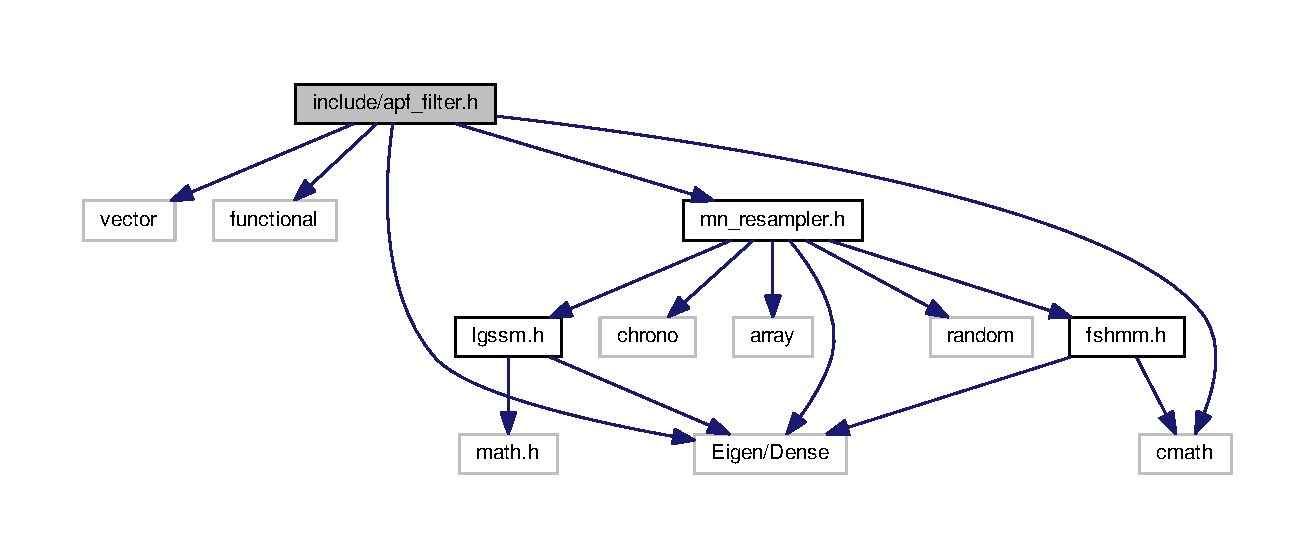
\includegraphics[width=350pt]{apf__filter_8h__incl}
\end{center}
\end{figure}
\subsection*{Classes}
\begin{DoxyCompactItemize}
\item 
class \hyperlink{classAPFFilter}{A\+P\+F\+Filter}
\begin{DoxyCompactList}\small\item\em A base-\/class for Auxiliary Particle Filtering. Filtering only, no smoothing. \end{DoxyCompactList}\end{DoxyCompactItemize}
\subsection*{Typedefs}
\begin{DoxyCompactItemize}
\item 
typedef Eigen\+::\+Matrix$<$ double, Eigen\+::\+Dynamic, 1 $>$ \hyperlink{apf__filter_8h_a4c7df05c6f5e8a0d15ae14bcdbc07152}{Vec}
\item 
typedef Eigen\+::\+Matrix$<$ double, Eigen\+::\+Dynamic, Eigen\+::\+Dynamic $>$ \hyperlink{apf__filter_8h_ae601f56a556993079f730483c574356f}{Mat}
\end{DoxyCompactItemize}
\subsection*{Enumerations}
\begin{DoxyCompactItemize}
\item 
enum \hyperlink{apf__filter_8h_a187a7338bc8872e7607cf1ea4ffed47b}{A\+P\+F\+Resamp\+Style} \{ \\*
{\bfseries everytime\+\_\+multinomial}, 
{\bfseries never}, 
{\bfseries ess\+\_\+multinomial}, 
{\bfseries everytime\+\_\+multinomial}, 
\\*
{\bfseries never}, 
{\bfseries ess\+\_\+multinomial}
 \}
\end{DoxyCompactItemize}


\subsection{Detailed Description}
A base class for Auxiliary Particle Filtering. Inherit from this if you want to use an A\+PF for your state space model. Filtering only, no smoothing. 



\subsection{Typedef Documentation}
\index{apf\+\_\+filter.\+h@{apf\+\_\+filter.\+h}!Mat@{Mat}}
\index{Mat@{Mat}!apf\+\_\+filter.\+h@{apf\+\_\+filter.\+h}}
\subsubsection[{\texorpdfstring{Mat}{Mat}}]{\setlength{\rightskip}{0pt plus 5cm}typedef Eigen\+::\+Matrix$<$ double, Eigen\+::\+Dynamic, Eigen\+::\+Dynamic $>$ {\bf Mat}}\hypertarget{apf__filter_8h_ae601f56a556993079f730483c574356f}{}\label{apf__filter_8h_ae601f56a556993079f730483c574356f}
typedef for linear algebra stuff \index{apf\+\_\+filter.\+h@{apf\+\_\+filter.\+h}!Vec@{Vec}}
\index{Vec@{Vec}!apf\+\_\+filter.\+h@{apf\+\_\+filter.\+h}}
\subsubsection[{\texorpdfstring{Vec}{Vec}}]{\setlength{\rightskip}{0pt plus 5cm}typedef Eigen\+::\+Matrix$<$ double, Eigen\+::\+Dynamic, 1 $>$ {\bf Vec}}\hypertarget{apf__filter_8h_a4c7df05c6f5e8a0d15ae14bcdbc07152}{}\label{apf__filter_8h_a4c7df05c6f5e8a0d15ae14bcdbc07152}
typedef for linear algebra stuff 

\subsection{Enumeration Type Documentation}
\index{apf\+\_\+filter.\+h@{apf\+\_\+filter.\+h}!A\+P\+F\+Resamp\+Style@{A\+P\+F\+Resamp\+Style}}
\index{A\+P\+F\+Resamp\+Style@{A\+P\+F\+Resamp\+Style}!apf\+\_\+filter.\+h@{apf\+\_\+filter.\+h}}
\subsubsection[{\texorpdfstring{A\+P\+F\+Resamp\+Style}{APFResampStyle}}]{\setlength{\rightskip}{0pt plus 5cm}enum {\bf A\+P\+F\+Resamp\+Style}\hspace{0.3cm}{\ttfamily [strong]}}\hypertarget{apf__filter_8h_a187a7338bc8872e7607cf1ea4ffed47b}{}\label{apf__filter_8h_a187a7338bc8872e7607cf1ea4ffed47b}
enum class for the type of resampling to be performed 
\hypertarget{apf__smooth_8h}{}\section{include/apf\+\_\+smooth.h File Reference}
\label{apf__smooth_8h}\index{include/apf\+\_\+smooth.\+h@{include/apf\+\_\+smooth.\+h}}


A base class for Auxiliary Particle Filtering. Inherit from this if you want to use an A\+PF for your state space model.  


{\ttfamily \#include $<$vector$>$}\\*
{\ttfamily \#include $<$functional$>$}\\*
{\ttfamily \#include $<$Eigen/\+Dense$>$}\\*
{\ttfamily \#include \char`\"{}multinomial\+\_\+resampler.\+h\char`\"{}}\\*
Include dependency graph for apf\+\_\+smooth.\+h\+:\nopagebreak
\begin{figure}[H]
\begin{center}
\leavevmode
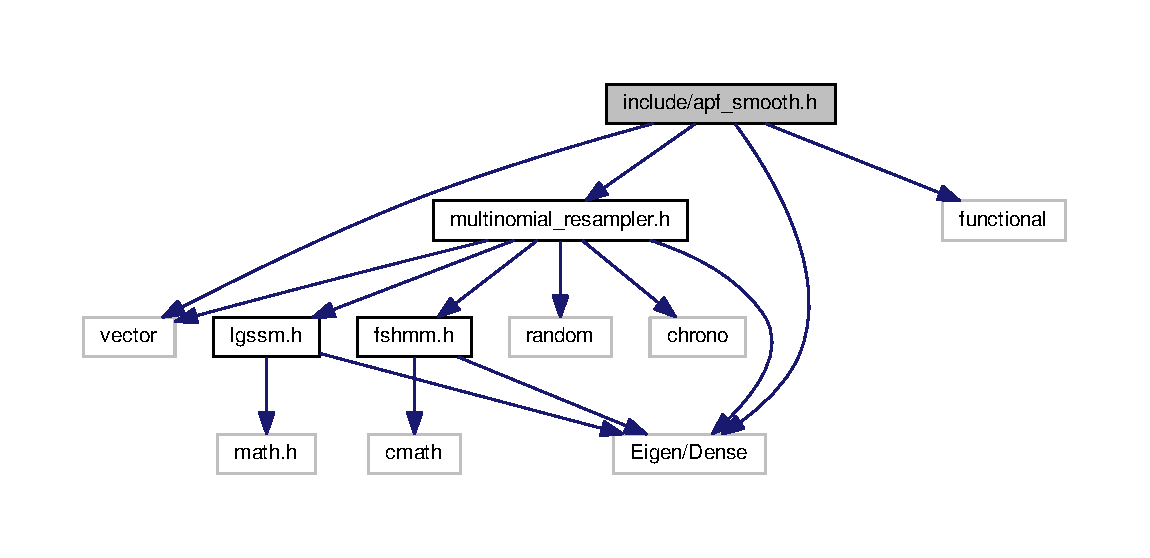
\includegraphics[width=350pt]{apf__smooth_8h__incl}
\end{center}
\end{figure}
\subsection*{Classes}
\begin{DoxyCompactItemize}
\item 
class \hyperlink{classAPFSmoother}{A\+P\+F\+Smoother}
\begin{DoxyCompactList}\small\item\em A base-\/class for Auxiliary Particle Filtering. Particle smoothing only; no filtering. \end{DoxyCompactList}\end{DoxyCompactItemize}
\subsection*{Typedefs}
\begin{DoxyCompactItemize}
\item 
typedef Eigen\+::\+Matrix$<$ double, Eigen\+::\+Dynamic, 1 $>$ \hyperlink{apf__smooth_8h_a4c7df05c6f5e8a0d15ae14bcdbc07152}{Vec}
\item 
typedef Eigen\+::\+Matrix$<$ double, Eigen\+::\+Dynamic, Eigen\+::\+Dynamic $>$ \hyperlink{apf__smooth_8h_ae601f56a556993079f730483c574356f}{Mat}
\end{DoxyCompactItemize}
\subsection*{Enumerations}
\begin{DoxyCompactItemize}
\item 
enum \hyperlink{apf__smooth_8h_a187a7338bc8872e7607cf1ea4ffed47b}{A\+P\+F\+Resamp\+Style} \{ \\*
{\bfseries everytime\+\_\+multinomial}, 
{\bfseries never}, 
{\bfseries ess\+\_\+multinomial}, 
{\bfseries everytime\+\_\+multinomial}, 
\\*
{\bfseries never}, 
{\bfseries ess\+\_\+multinomial}
 \}
\end{DoxyCompactItemize}


\subsection{Detailed Description}
A base class for Auxiliary Particle Filtering. Inherit from this if you want to use an A\+PF for your state space model. 



\subsection{Typedef Documentation}
\index{apf\+\_\+smooth.\+h@{apf\+\_\+smooth.\+h}!Mat@{Mat}}
\index{Mat@{Mat}!apf\+\_\+smooth.\+h@{apf\+\_\+smooth.\+h}}
\subsubsection[{\texorpdfstring{Mat}{Mat}}]{\setlength{\rightskip}{0pt plus 5cm}typedef Eigen\+::\+Matrix$<$ double, Eigen\+::\+Dynamic, Eigen\+::\+Dynamic $>$ {\bf Mat}}\hypertarget{apf__smooth_8h_ae601f56a556993079f730483c574356f}{}\label{apf__smooth_8h_ae601f56a556993079f730483c574356f}
typedef for linear algebra stuff \index{apf\+\_\+smooth.\+h@{apf\+\_\+smooth.\+h}!Vec@{Vec}}
\index{Vec@{Vec}!apf\+\_\+smooth.\+h@{apf\+\_\+smooth.\+h}}
\subsubsection[{\texorpdfstring{Vec}{Vec}}]{\setlength{\rightskip}{0pt plus 5cm}typedef Eigen\+::\+Matrix$<$ double, Eigen\+::\+Dynamic, 1 $>$ {\bf Vec}}\hypertarget{apf__smooth_8h_a4c7df05c6f5e8a0d15ae14bcdbc07152}{}\label{apf__smooth_8h_a4c7df05c6f5e8a0d15ae14bcdbc07152}
typedef for linear algebra stuff 

\subsection{Enumeration Type Documentation}
\index{apf\+\_\+smooth.\+h@{apf\+\_\+smooth.\+h}!A\+P\+F\+Resamp\+Style@{A\+P\+F\+Resamp\+Style}}
\index{A\+P\+F\+Resamp\+Style@{A\+P\+F\+Resamp\+Style}!apf\+\_\+smooth.\+h@{apf\+\_\+smooth.\+h}}
\subsubsection[{\texorpdfstring{A\+P\+F\+Resamp\+Style}{APFResampStyle}}]{\setlength{\rightskip}{0pt plus 5cm}enum {\bf A\+P\+F\+Resamp\+Style}\hspace{0.3cm}{\ttfamily [strong]}}\hypertarget{apf__smooth_8h_a187a7338bc8872e7607cf1ea4ffed47b}{}\label{apf__smooth_8h_a187a7338bc8872e7607cf1ea4ffed47b}
enum class for the type of resampling to be performed 
\hypertarget{bootstrap__filter_8h}{}\section{include/bootstrap\+\_\+filter.h File Reference}
\label{bootstrap__filter_8h}\index{include/bootstrap\+\_\+filter.\+h@{include/bootstrap\+\_\+filter.\+h}}
{\ttfamily \#include $<$Eigen/\+Dense$>$}\\*
{\ttfamily \#include \char`\"{}multinomial\+\_\+resampler.\+h\char`\"{}}\\*
Include dependency graph for bootstrap\+\_\+filter.\+h\+:\nopagebreak
\begin{figure}[H]
\begin{center}
\leavevmode
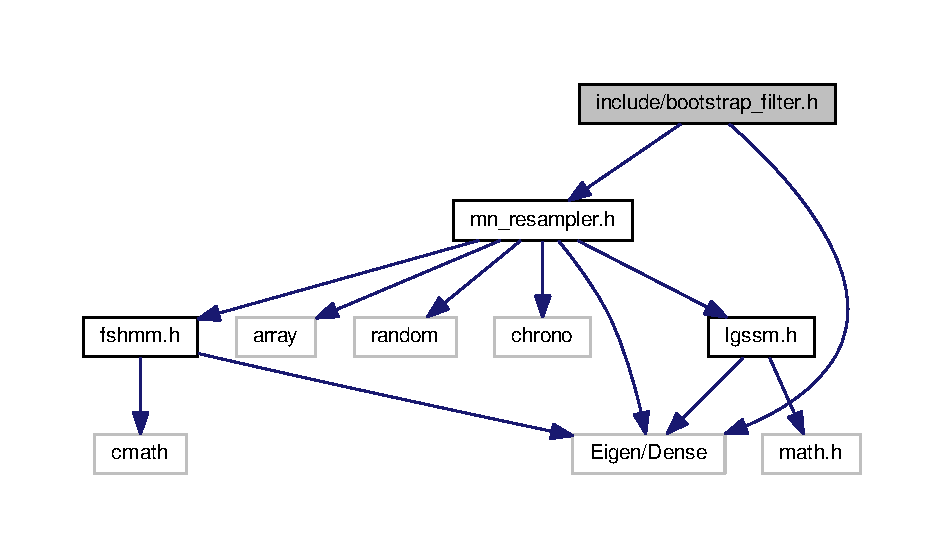
\includegraphics[width=350pt]{bootstrap__filter_8h__incl}
\end{center}
\end{figure}
\subsection*{Classes}
\begin{DoxyCompactItemize}
\item 
class \hyperlink{classBSFilter}{B\+S\+Filter}
\begin{DoxyCompactList}\small\item\em A base-\/class for Bootstrap Filtering (S\+I\+SR with naive proposals). This class is a bit faster because it. \end{DoxyCompactList}\end{DoxyCompactItemize}
\subsection*{Typedefs}
\begin{DoxyCompactItemize}
\item 
typedef Eigen\+::\+Matrix$<$ double, Eigen\+::\+Dynamic, 1 $>$ \hyperlink{bootstrap__filter_8h_a4c7df05c6f5e8a0d15ae14bcdbc07152}{Vec}
\item 
typedef Eigen\+::\+Matrix$<$ double, Eigen\+::\+Dynamic, Eigen\+::\+Dynamic $>$ \hyperlink{bootstrap__filter_8h_ae601f56a556993079f730483c574356f}{Mat}
\end{DoxyCompactItemize}
\subsection*{Enumerations}
\begin{DoxyCompactItemize}
\item 
enum \hyperlink{bootstrap__filter_8h_a476b3b5754056a34ac843629c9570b49}{B\+S\+Resamp\+Style} \{ {\bfseries everytime\+\_\+multinomial}, 
{\bfseries never}, 
{\bfseries ess\+\_\+multinomial}
 \}
\end{DoxyCompactItemize}


\subsection{Typedef Documentation}
\index{bootstrap\+\_\+filter.\+h@{bootstrap\+\_\+filter.\+h}!Mat@{Mat}}
\index{Mat@{Mat}!bootstrap\+\_\+filter.\+h@{bootstrap\+\_\+filter.\+h}}
\subsubsection[{\texorpdfstring{Mat}{Mat}}]{\setlength{\rightskip}{0pt plus 5cm}typedef Eigen\+::\+Matrix$<$ double, Eigen\+::\+Dynamic, Eigen\+::\+Dynamic $>$ {\bf Mat}}\hypertarget{bootstrap__filter_8h_ae601f56a556993079f730483c574356f}{}\label{bootstrap__filter_8h_ae601f56a556993079f730483c574356f}
typedef for linear algebra stuff \index{bootstrap\+\_\+filter.\+h@{bootstrap\+\_\+filter.\+h}!Vec@{Vec}}
\index{Vec@{Vec}!bootstrap\+\_\+filter.\+h@{bootstrap\+\_\+filter.\+h}}
\subsubsection[{\texorpdfstring{Vec}{Vec}}]{\setlength{\rightskip}{0pt plus 5cm}typedef Eigen\+::\+Matrix$<$ double, Eigen\+::\+Dynamic, 1 $>$ {\bf Vec}}\hypertarget{bootstrap__filter_8h_a4c7df05c6f5e8a0d15ae14bcdbc07152}{}\label{bootstrap__filter_8h_a4c7df05c6f5e8a0d15ae14bcdbc07152}
typedef for linear algebra stuff 

\subsection{Enumeration Type Documentation}
\index{bootstrap\+\_\+filter.\+h@{bootstrap\+\_\+filter.\+h}!B\+S\+Resamp\+Style@{B\+S\+Resamp\+Style}}
\index{B\+S\+Resamp\+Style@{B\+S\+Resamp\+Style}!bootstrap\+\_\+filter.\+h@{bootstrap\+\_\+filter.\+h}}
\subsubsection[{\texorpdfstring{B\+S\+Resamp\+Style}{BSResampStyle}}]{\setlength{\rightskip}{0pt plus 5cm}enum {\bf B\+S\+Resamp\+Style}\hspace{0.3cm}{\ttfamily [strong]}}\hypertarget{bootstrap__filter_8h_a476b3b5754056a34ac843629c9570b49}{}\label{bootstrap__filter_8h_a476b3b5754056a34ac843629c9570b49}
enum class for the type of resampling to be performed 
\hypertarget{densities_8h}{}\section{include/densities.h File Reference}
\label{densities_8h}\index{include/densities.\+h@{include/densities.\+h}}


Can sample from a distribution with fixed mean and covariance, fixed mean only, fixed covariance only, or nothing fixed.  


{\ttfamily \#include $<$chrono$>$}\\*
{\ttfamily \#include $<$Eigen/\+Dense$>$}\\*
{\ttfamily \#include $<$random$>$}\\*
Include dependency graph for densities.\+h\+:\nopagebreak
\begin{figure}[H]
\begin{center}
\leavevmode
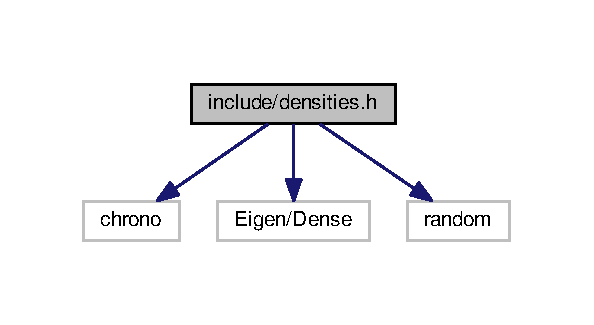
\includegraphics[width=285pt]{densities_8h__incl}
\end{center}
\end{figure}
This graph shows which files directly or indirectly include this file\+:
\nopagebreak
\begin{figure}[H]
\begin{center}
\leavevmode
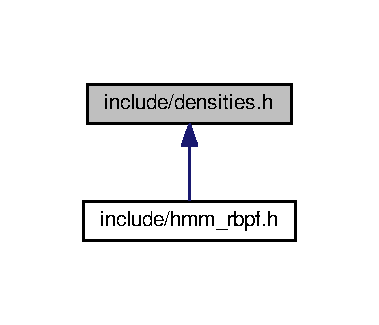
\includegraphics[width=350pt]{densities_8h__dep__incl}
\end{center}
\end{figure}
\subsection*{Classes}
\begin{DoxyCompactItemize}
\item 
class \hyperlink{classdensities_1_1MVNSampler}{densities\+::\+M\+V\+N\+Sampler}
\begin{DoxyCompactList}\small\item\em A class that performs sampling from a multivariate normal distribution. \end{DoxyCompactList}\item 
class \hyperlink{classdensities_1_1UniformSampler}{densities\+::\+Uniform\+Sampler}
\begin{DoxyCompactList}\small\item\em A class that performs sampling from a continuous uniform distribution. \end{DoxyCompactList}\end{DoxyCompactItemize}
\subsection*{Typedefs}
\begin{DoxyCompactItemize}
\item 
typedef Eigen\+::\+Matrix$<$ double, Eigen\+::\+Dynamic, 1 $>$ {\bfseries Vec}\hypertarget{densities_8h_a4c7df05c6f5e8a0d15ae14bcdbc07152}{}\label{densities_8h_a4c7df05c6f5e8a0d15ae14bcdbc07152}

\item 
typedef Eigen\+::\+Matrix$<$ double, Eigen\+::\+Dynamic, Eigen\+::\+Dynamic $>$ {\bfseries Mat}\hypertarget{densities_8h_ae601f56a556993079f730483c574356f}{}\label{densities_8h_ae601f56a556993079f730483c574356f}

\end{DoxyCompactItemize}
\subsection*{Functions}
\begin{DoxyCompactItemize}
\item 
const double {\bfseries densities\+::inv\+\_\+sqrt\+\_\+2pi} (0.\+3989422804014327)\hypertarget{densities_8h_a50fd069caa24dac797922e8af6ed68e2}{}\label{densities_8h_a50fd069caa24dac797922e8af6ed68e2}

\item 
const double {\bfseries densities\+::sqrt\+\_\+two\+\_\+over\+\_\+pi} (0.\+797884560802865)\hypertarget{densities_8h_a36eeab0ef3c0cbfa190716631c183f17}{}\label{densities_8h_a36eeab0ef3c0cbfa190716631c183f17}

\item 
const double {\bfseries densities\+::log\+\_\+two\+\_\+pi} (1.\+83787706640935)\hypertarget{densities_8h_ae55ae08fac65b33b193ed333538dd340}{}\label{densities_8h_ae55ae08fac65b33b193ed333538dd340}

\item 
const double {\bfseries densities\+::log\+\_\+two\+\_\+over\+\_\+pi} (-\/0.\+451582705289455)\hypertarget{densities_8h_a45b1879e50e22cb4ee16e2b9b86c3b14}{}\label{densities_8h_a45b1879e50e22cb4ee16e2b9b86c3b14}

\item 
double \hyperlink{densities_8h_a9e47ab78e9b67622852378c44b6ccc2d}{densities\+::eval\+Multiv\+Norm} (const Vec \&x, const Vec \&mean\+Vec, const Mat \&cov\+Mat, bool log=false)
\begin{DoxyCompactList}\small\item\em Evaluates the multivariate normal density. \end{DoxyCompactList}\item 
double \hyperlink{densities_8h_a0c5bdd99b4d611a05cb2cf2615c4c07a}{densities\+::eval\+Univ\+Beta} (const double \&x, const double \&alpha, const double \&beta, bool log=false)
\begin{DoxyCompactList}\small\item\em Evaluates the univariate Beta density. \end{DoxyCompactList}\item 
double \hyperlink{densities_8h_a6a348ae64240f768da13e50a1d30eb69}{densities\+::eval\+Univ\+Inv\+Gamma} (const double \&x, const double \&alpha, const double \&beta, bool log=false)
\begin{DoxyCompactList}\small\item\em Evaluates the univariate Inverse Gamma density. \end{DoxyCompactList}\item 
double \hyperlink{densities_8h_a7bdccb2414aa07d7d0710b459b5de9cd}{densities\+::eval\+Univ\+Half\+Norm} (const double \&x, const double \&sigma\+Sqd, bool log=false)
\begin{DoxyCompactList}\small\item\em Evaluates the half-\/normal density. \end{DoxyCompactList}\end{DoxyCompactItemize}


\subsection{Detailed Description}
Can sample from a distribution with fixed mean and covariance, fixed mean only, fixed covariance only, or nothing fixed. 



\subsection{Function Documentation}
\index{densities.\+h@{densities.\+h}!eval\+Multiv\+Norm@{eval\+Multiv\+Norm}}
\index{eval\+Multiv\+Norm@{eval\+Multiv\+Norm}!densities.\+h@{densities.\+h}}
\subsubsection[{\texorpdfstring{eval\+Multiv\+Norm(const Vec \&x, const Vec \&mean\+Vec, const Mat \&cov\+Mat, bool log=false)}{evalMultivNorm(const Vec &x, const Vec &meanVec, const Mat &covMat, bool log=false)}}]{\setlength{\rightskip}{0pt plus 5cm}double densities\+::eval\+Multiv\+Norm (
\begin{DoxyParamCaption}
\item[{const Vec \&}]{x, }
\item[{const Vec \&}]{mean\+Vec, }
\item[{const Mat \&}]{cov\+Mat, }
\item[{bool}]{log = {\ttfamily false}}
\end{DoxyParamCaption}
)}\hypertarget{densities_8h_file_a9e47ab78e9b67622852378c44b6ccc2d}{}\label{densities_8h_file_a9e47ab78e9b67622852378c44b6ccc2d}


Evaluates the multivariate normal density. 


\begin{DoxyParams}{Parameters}
{\em x} & \\
\hline
{\em mean\+Vec} & the mean vector \\
\hline
{\em cov\+Mat} & the positive definite, symmetric covariance matrix \\
\hline
{\em log} & true if you want to return the log density. false otherwise \\
\hline
\end{DoxyParams}
\begin{DoxyReturn}{Returns}
a double 
\end{DoxyReturn}
\index{densities.\+h@{densities.\+h}!eval\+Univ\+Beta@{eval\+Univ\+Beta}}
\index{eval\+Univ\+Beta@{eval\+Univ\+Beta}!densities.\+h@{densities.\+h}}
\subsubsection[{\texorpdfstring{eval\+Univ\+Beta(const double \&x, const double \&alpha, const double \&beta, bool log=false)}{evalUnivBeta(const double &x, const double &alpha, const double &beta, bool log=false)}}]{\setlength{\rightskip}{0pt plus 5cm}double densities\+::eval\+Univ\+Beta (
\begin{DoxyParamCaption}
\item[{const double \&}]{x, }
\item[{const double \&}]{alpha, }
\item[{const double \&}]{beta, }
\item[{bool}]{log = {\ttfamily false}}
\end{DoxyParamCaption}
)}\hypertarget{densities_8h_file_a0c5bdd99b4d611a05cb2cf2615c4c07a}{}\label{densities_8h_file_a0c5bdd99b4d611a05cb2cf2615c4c07a}


Evaluates the univariate Beta density. 


\begin{DoxyParams}{Parameters}
{\em x} & the point \\
\hline
{\em alpha} & parameter 1 \\
\hline
{\em beta} & parameter 2 \\
\hline
\end{DoxyParams}
\begin{DoxyReturn}{Returns}
double evaluation. 
\end{DoxyReturn}
\index{densities.\+h@{densities.\+h}!eval\+Univ\+Half\+Norm@{eval\+Univ\+Half\+Norm}}
\index{eval\+Univ\+Half\+Norm@{eval\+Univ\+Half\+Norm}!densities.\+h@{densities.\+h}}
\subsubsection[{\texorpdfstring{eval\+Univ\+Half\+Norm(const double \&x, const double \&sigma\+Sqd, bool log=false)}{evalUnivHalfNorm(const double &x, const double &sigmaSqd, bool log=false)}}]{\setlength{\rightskip}{0pt plus 5cm}double densities\+::eval\+Univ\+Half\+Norm (
\begin{DoxyParamCaption}
\item[{const double \&}]{x, }
\item[{const double \&}]{sigma\+Sqd, }
\item[{bool}]{log = {\ttfamily false}}
\end{DoxyParamCaption}
)}\hypertarget{densities_8h_file_a7bdccb2414aa07d7d0710b459b5de9cd}{}\label{densities_8h_file_a7bdccb2414aa07d7d0710b459b5de9cd}


Evaluates the half-\/normal density. 


\begin{DoxyParams}{Parameters}
{\em x} & the point you\textquotesingle{}re evaluating at \\
\hline
{\em sigma\+Sqd} & the scale parameter \\
\hline
\end{DoxyParams}
\begin{DoxyReturn}{Returns}
double evaluation. 
\end{DoxyReturn}
\index{densities.\+h@{densities.\+h}!eval\+Univ\+Inv\+Gamma@{eval\+Univ\+Inv\+Gamma}}
\index{eval\+Univ\+Inv\+Gamma@{eval\+Univ\+Inv\+Gamma}!densities.\+h@{densities.\+h}}
\subsubsection[{\texorpdfstring{eval\+Univ\+Inv\+Gamma(const double \&x, const double \&alpha, const double \&beta, bool log=false)}{evalUnivInvGamma(const double &x, const double &alpha, const double &beta, bool log=false)}}]{\setlength{\rightskip}{0pt plus 5cm}double densities\+::eval\+Univ\+Inv\+Gamma (
\begin{DoxyParamCaption}
\item[{const double \&}]{x, }
\item[{const double \&}]{alpha, }
\item[{const double \&}]{beta, }
\item[{bool}]{log = {\ttfamily false}}
\end{DoxyParamCaption}
)}\hypertarget{densities_8h_file_a6a348ae64240f768da13e50a1d30eb69}{}\label{densities_8h_file_a6a348ae64240f768da13e50a1d30eb69}


Evaluates the univariate Inverse Gamma density. 


\begin{DoxyParams}{Parameters}
{\em x} & the point \\
\hline
{\em alpha} & shape parameter \\
\hline
{\em beta} & rate parameter \\
\hline
\end{DoxyParams}
\begin{DoxyReturn}{Returns}
double evaluation. 
\end{DoxyReturn}

\hypertarget{hmm__rbpf_8h}{}\section{include/hmm\+\_\+rbpf.h File Reference}
\label{hmm__rbpf_8h}\index{include/hmm\+\_\+rbpf.\+h@{include/hmm\+\_\+rbpf.\+h}}


Rao-\/\+Blackwellized particle filtering where the innder models are discrete state hmms.  


{\ttfamily \#include $<$Eigen/\+Dense$>$}\\*
{\ttfamily \#include $<$vector$>$}\\*
{\ttfamily \#include $<$functional$>$}\\*
{\ttfamily \#include \char`\"{}fshmm.\+h\char`\"{}}\\*
{\ttfamily \#include \char`\"{}multinomial\+\_\+resampler.\+h\char`\"{}}\\*
{\ttfamily \#include \char`\"{}densities.\+h\char`\"{}}\\*
Include dependency graph for hmm\+\_\+rbpf.\+h\+:\nopagebreak
\begin{figure}[H]
\begin{center}
\leavevmode
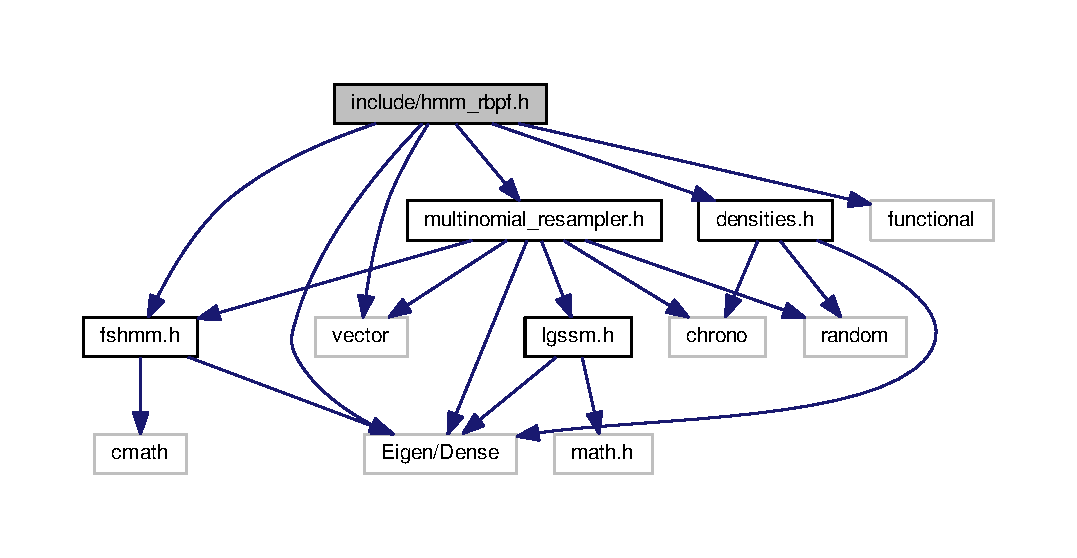
\includegraphics[width=350pt]{hmm__rbpf_8h__incl}
\end{center}
\end{figure}
\subsection*{Classes}
\begin{DoxyCompactItemize}
\item 
class \hyperlink{classHmm__Rbpf}{Hmm\+\_\+\+Rbpf}
\begin{DoxyCompactList}\small\item\em A base-\/class for H\+MM Rao-\/\+Blackwellized Particle Filtering. \end{DoxyCompactList}\end{DoxyCompactItemize}
\subsection*{Enumerations}
\begin{DoxyCompactItemize}
\item 
enum \hyperlink{hmm__rbpf_8h_aa0729d190f1f8b76b203466a41f1505f}{H\+M\+M\+R\+B\+P\+F\+Resamp\+Style} \{ {\bfseries everytime\+\_\+multinomial}, 
{\bfseries never}, 
{\bfseries ess\+\_\+multinomial}
 \}
\end{DoxyCompactItemize}


\subsection{Detailed Description}
Rao-\/\+Blackwellized particle filtering where the innder models are discrete state hmms. 



\subsection{Enumeration Type Documentation}
\index{hmm\+\_\+rbpf.\+h@{hmm\+\_\+rbpf.\+h}!H\+M\+M\+R\+B\+P\+F\+Resamp\+Style@{H\+M\+M\+R\+B\+P\+F\+Resamp\+Style}}
\index{H\+M\+M\+R\+B\+P\+F\+Resamp\+Style@{H\+M\+M\+R\+B\+P\+F\+Resamp\+Style}!hmm\+\_\+rbpf.\+h@{hmm\+\_\+rbpf.\+h}}
\subsubsection[{\texorpdfstring{H\+M\+M\+R\+B\+P\+F\+Resamp\+Style}{HMMRBPFResampStyle}}]{\setlength{\rightskip}{0pt plus 5cm}enum {\bf H\+M\+M\+R\+B\+P\+F\+Resamp\+Style}\hspace{0.3cm}{\ttfamily [strong]}}\hypertarget{hmm__rbpf_8h_aa0729d190f1f8b76b203466a41f1505f}{}\label{hmm__rbpf_8h_aa0729d190f1f8b76b203466a41f1505f}
enum class for the type of resampling to be performed 
\hypertarget{kalman__rbpf_8h}{}\section{include/kalman\+\_\+rbpf.h File Reference}
\label{kalman__rbpf_8h}\index{include/kalman\+\_\+rbpf.\+h@{include/kalman\+\_\+rbpf.\+h}}


Rao-\/\+Blackwellized Particle Filter with Linear Gaussian submodel.  


{\ttfamily \#include $<$vector$>$}\\*
{\ttfamily \#include $<$Eigen/\+Dense$>$}\\*
{\ttfamily \#include \char`\"{}lgssm.\+h\char`\"{}}\\*
{\ttfamily \#include \char`\"{}multinomial\+\_\+resampler.\+h\char`\"{}}\\*
Include dependency graph for kalman\+\_\+rbpf.\+h\+:\nopagebreak
\begin{figure}[H]
\begin{center}
\leavevmode
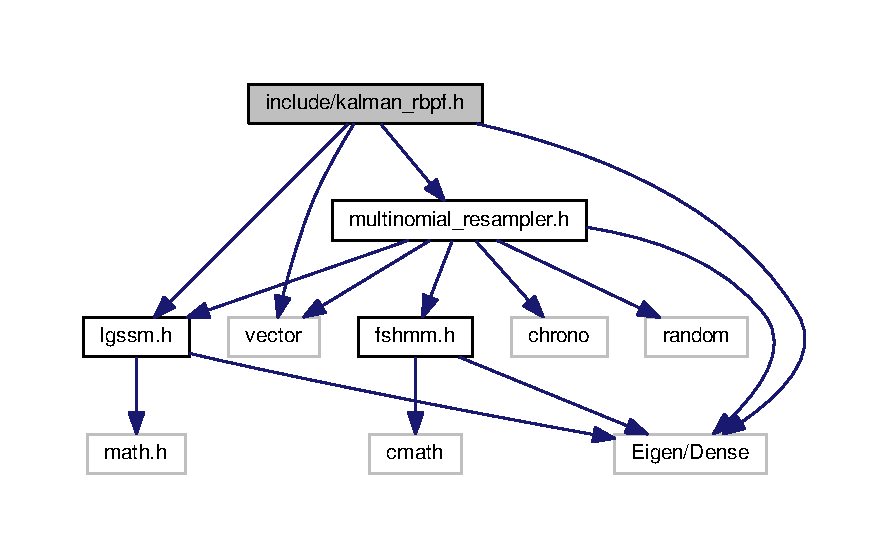
\includegraphics[width=350pt]{kalman__rbpf_8h__incl}
\end{center}
\end{figure}
\subsection*{Classes}
\begin{DoxyCompactItemize}
\item 
class \hyperlink{classKalman__RBPF}{Kalman\+\_\+\+R\+B\+PF}
\begin{DoxyCompactList}\small\item\em A base-\/class for Kalman Rao-\/\+Blackwellized Particle Filtering. \end{DoxyCompactList}\end{DoxyCompactItemize}
\subsection*{Typedefs}
\begin{DoxyCompactItemize}
\item 
typedef Eigen\+::\+Matrix$<$ double, Eigen\+::\+Dynamic, 1 $>$ \hyperlink{kalman__rbpf_8h_a4c7df05c6f5e8a0d15ae14bcdbc07152}{Vec}
\item 
typedef Eigen\+::\+Matrix$<$ double, Eigen\+::\+Dynamic, Eigen\+::\+Dynamic $>$ \hyperlink{kalman__rbpf_8h_ae601f56a556993079f730483c574356f}{Mat}
\end{DoxyCompactItemize}
\subsection*{Enumerations}
\begin{DoxyCompactItemize}
\item 
enum \hyperlink{kalman__rbpf_8h_ad3790b392be9413a27de33728aad31e2}{R\+B\+P\+F\+Resamp\+Style} \{ {\bfseries everytime\+\_\+multinomial}, 
{\bfseries never}, 
{\bfseries ess\+\_\+multinomial}
 \}
\end{DoxyCompactItemize}


\subsection{Detailed Description}
Rao-\/\+Blackwellized Particle Filter with Linear Gaussian submodel. 



\subsection{Typedef Documentation}
\index{kalman\+\_\+rbpf.\+h@{kalman\+\_\+rbpf.\+h}!Mat@{Mat}}
\index{Mat@{Mat}!kalman\+\_\+rbpf.\+h@{kalman\+\_\+rbpf.\+h}}
\subsubsection[{\texorpdfstring{Mat}{Mat}}]{\setlength{\rightskip}{0pt plus 5cm}typedef Eigen\+::\+Matrix$<$ double, Eigen\+::\+Dynamic, Eigen\+::\+Dynamic $>$ {\bf Mat}}\hypertarget{kalman__rbpf_8h_ae601f56a556993079f730483c574356f}{}\label{kalman__rbpf_8h_ae601f56a556993079f730483c574356f}
typedef for linear algebra stuff \index{kalman\+\_\+rbpf.\+h@{kalman\+\_\+rbpf.\+h}!Vec@{Vec}}
\index{Vec@{Vec}!kalman\+\_\+rbpf.\+h@{kalman\+\_\+rbpf.\+h}}
\subsubsection[{\texorpdfstring{Vec}{Vec}}]{\setlength{\rightskip}{0pt plus 5cm}typedef Eigen\+::\+Matrix$<$ double, Eigen\+::\+Dynamic, 1 $>$ {\bf Vec}}\hypertarget{kalman__rbpf_8h_a4c7df05c6f5e8a0d15ae14bcdbc07152}{}\label{kalman__rbpf_8h_a4c7df05c6f5e8a0d15ae14bcdbc07152}
typedef for linear algebra stuff 

\subsection{Enumeration Type Documentation}
\index{kalman\+\_\+rbpf.\+h@{kalman\+\_\+rbpf.\+h}!R\+B\+P\+F\+Resamp\+Style@{R\+B\+P\+F\+Resamp\+Style}}
\index{R\+B\+P\+F\+Resamp\+Style@{R\+B\+P\+F\+Resamp\+Style}!kalman\+\_\+rbpf.\+h@{kalman\+\_\+rbpf.\+h}}
\subsubsection[{\texorpdfstring{R\+B\+P\+F\+Resamp\+Style}{RBPFResampStyle}}]{\setlength{\rightskip}{0pt plus 5cm}enum {\bf R\+B\+P\+F\+Resamp\+Style}\hspace{0.3cm}{\ttfamily [strong]}}\hypertarget{kalman__rbpf_8h_ad3790b392be9413a27de33728aad31e2}{}\label{kalman__rbpf_8h_ad3790b392be9413a27de33728aad31e2}
enum class for the type of resampling to be performed 
\hypertarget{multinomial__resampler_8h}{}\section{include/multinomial\+\_\+resampler.h File Reference}
\label{multinomial__resampler_8h}\index{include/multinomial\+\_\+resampler.\+h@{include/multinomial\+\_\+resampler.\+h}}


A class used for all the multinomial resampling in any model. Keep in mind this is usually implemented by the base classes themselves, and so this would mean they are not touched by the typical end-\/user.  


{\ttfamily \#include $<$Eigen/\+Dense$>$}\\*
{\ttfamily \#include $<$vector$>$}\\*
{\ttfamily \#include $<$random$>$}\\*
{\ttfamily \#include $<$chrono$>$}\\*
{\ttfamily \#include \char`\"{}lgssm.\+h\char`\"{}}\\*
{\ttfamily \#include \char`\"{}fshmm.\+h\char`\"{}}\\*
Include dependency graph for multinomial\+\_\+resampler.\+h\+:\nopagebreak
\begin{figure}[H]
\begin{center}
\leavevmode
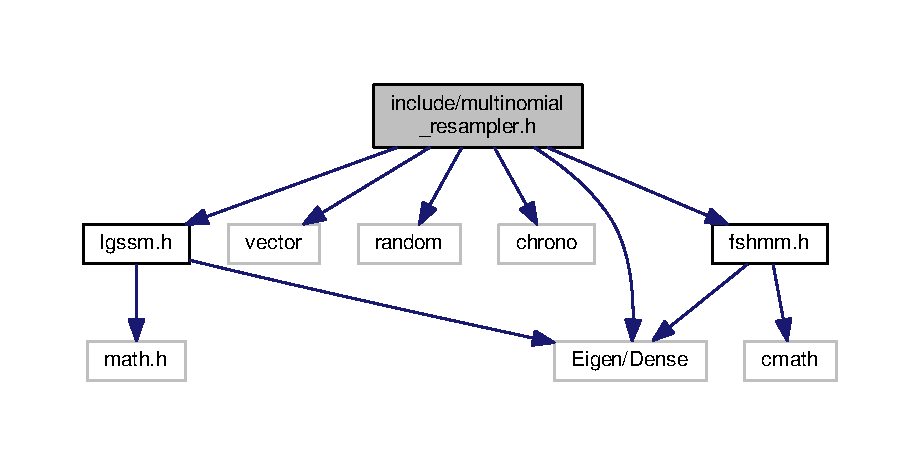
\includegraphics[width=350pt]{multinomial__resampler_8h__incl}
\end{center}
\end{figure}
This graph shows which files directly or indirectly include this file\+:\nopagebreak
\begin{figure}[H]
\begin{center}
\leavevmode
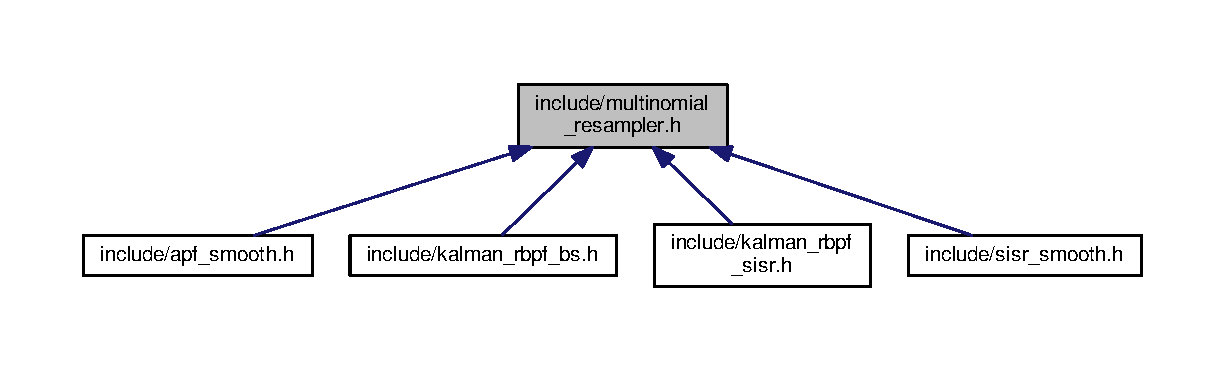
\includegraphics[width=350pt]{multinomial__resampler_8h__dep__incl}
\end{center}
\end{figure}
\subsection*{Classes}
\begin{DoxyCompactItemize}
\item 
class \hyperlink{classMultinomResamp}{Multinom\+Resamp}
\begin{DoxyCompactList}\small\item\em A class for Multinomial Resampling. \end{DoxyCompactList}\end{DoxyCompactItemize}
\subsection*{Typedefs}
\begin{DoxyCompactItemize}
\item 
typedef Eigen\+::\+Matrix$<$ double, Eigen\+::\+Dynamic, 1 $>$ \hyperlink{multinomial__resampler_8h_a360fe0c7b2382d504256a49473c3be26}{Vec}
\end{DoxyCompactItemize}


\subsection{Detailed Description}
A class used for all the multinomial resampling in any model. Keep in mind this is usually implemented by the base classes themselves, and so this would mean they are not touched by the typical end-\/user. 



\subsection{Typedef Documentation}
\index{multinomial\+\_\+resampler.\+h@{multinomial\+\_\+resampler.\+h}!Vec@{Vec}}
\index{Vec@{Vec}!multinomial\+\_\+resampler.\+h@{multinomial\+\_\+resampler.\+h}}
\subsubsection[{\texorpdfstring{Vec}{Vec}}]{\setlength{\rightskip}{0pt plus 5cm}typedef Eigen\+::\+Matrix$<$ double, Eigen\+::\+Dynamic, 1$>$ {\bf Vec}}\hypertarget{multinomial__resampler_8h_a360fe0c7b2382d504256a49473c3be26}{}\label{multinomial__resampler_8h_a360fe0c7b2382d504256a49473c3be26}
typedef for linear algebra stuff 
\hypertarget{pmfs_8h}{}\section{include/pmfs.h File Reference}
\label{pmfs_8h}\index{include/pmfs.\+h@{include/pmfs.\+h}}
{\ttfamily \#include $<$random$>$}\\*
{\ttfamily \#include $<$vector$>$}\\*
{\ttfamily \#include $<$chrono$>$}\\*
{\ttfamily \#include $<$Eigen/\+Dense$>$}\\*
Include dependency graph for pmfs.\+h\+:\nopagebreak
\begin{figure}[H]
\begin{center}
\leavevmode
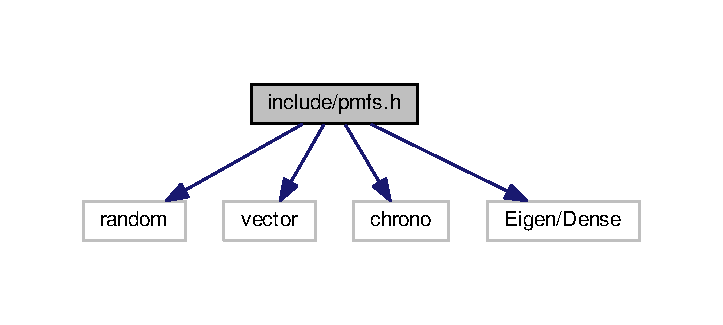
\includegraphics[width=347pt]{pmfs_8h__incl}
\end{center}
\end{figure}
\subsection*{Classes}
\begin{DoxyCompactItemize}
\item 
class \hyperlink{classpmfs_1_1DiscreteUnifSampler}{pmfs\+::\+Discrete\+Unif\+Sampler}
\begin{DoxyCompactList}\small\item\em A class that performs sampling from a discrete uniform distribution. \end{DoxyCompactList}\item 
class \hyperlink{classpmfs_1_1DiscreteCustomSampler}{pmfs\+::\+Discrete\+Custom\+Sampler}
\begin{DoxyCompactList}\small\item\em A class that performs sampling from a discrete custom distribution. \end{DoxyCompactList}\end{DoxyCompactItemize}
\subsection*{Typedefs}
\begin{DoxyCompactItemize}
\item 
typedef Eigen\+::\+Matrix$<$ double, Eigen\+::\+Dynamic, 1 $>$ \hyperlink{pmfs_8h_a4c7df05c6f5e8a0d15ae14bcdbc07152}{Vec}
\item 
typedef Eigen\+::\+Matrix$<$ double, Eigen\+::\+Dynamic, Eigen\+::\+Dynamic $>$ \hyperlink{pmfs_8h_ae601f56a556993079f730483c574356f}{Mat}
\end{DoxyCompactItemize}
\subsection*{Functions}
\begin{DoxyCompactItemize}
\item 
double \hyperlink{pmfs_8h_a21666e2a5112aa29a78053d23803f1b0}{pmfs\+::eval\+Discrete\+Unif} (const int \&x, const int \&k, bool log=false)
\begin{DoxyCompactList}\small\item\em Evaluates discrete uniform pmf. \end{DoxyCompactList}\end{DoxyCompactItemize}


\subsection{Typedef Documentation}
\index{pmfs.\+h@{pmfs.\+h}!Mat@{Mat}}
\index{Mat@{Mat}!pmfs.\+h@{pmfs.\+h}}
\subsubsection[{\texorpdfstring{Mat}{Mat}}]{\setlength{\rightskip}{0pt plus 5cm}typedef Eigen\+::\+Matrix$<$ double, Eigen\+::\+Dynamic, Eigen\+::\+Dynamic $>$ {\bf Mat}}\hypertarget{pmfs_8h_ae601f56a556993079f730483c574356f}{}\label{pmfs_8h_ae601f56a556993079f730483c574356f}
Shorthand typedef for Eigen\+::\+Matrix\+Xd \index{pmfs.\+h@{pmfs.\+h}!Vec@{Vec}}
\index{Vec@{Vec}!pmfs.\+h@{pmfs.\+h}}
\subsubsection[{\texorpdfstring{Vec}{Vec}}]{\setlength{\rightskip}{0pt plus 5cm}typedef Eigen\+::\+Matrix$<$ double, Eigen\+::\+Dynamic, 1 $>$ {\bf Vec}}\hypertarget{pmfs_8h_a4c7df05c6f5e8a0d15ae14bcdbc07152}{}\label{pmfs_8h_a4c7df05c6f5e8a0d15ae14bcdbc07152}
Shorthand typedef for Eigen\+::\+Vector\+Xd 

\subsection{Function Documentation}
\index{pmfs.\+h@{pmfs.\+h}!eval\+Discrete\+Unif@{eval\+Discrete\+Unif}}
\index{eval\+Discrete\+Unif@{eval\+Discrete\+Unif}!pmfs.\+h@{pmfs.\+h}}
\subsubsection[{\texorpdfstring{eval\+Discrete\+Unif(const int \&x, const int \&k, bool log=false)}{evalDiscreteUnif(const int &x, const int &k, bool log=false)}}]{\setlength{\rightskip}{0pt plus 5cm}double pmfs\+::eval\+Discrete\+Unif (
\begin{DoxyParamCaption}
\item[{const int \&}]{x, }
\item[{const int \&}]{k, }
\item[{bool}]{log = {\ttfamily false}}
\end{DoxyParamCaption}
)}\hypertarget{pmfs_8h_file_a21666e2a5112aa29a78053d23803f1b0}{}\label{pmfs_8h_file_a21666e2a5112aa29a78053d23803f1b0}


Evaluates discrete uniform pmf. 


\begin{DoxyParams}{Parameters}
{\em x} & the hypothetical value of a rv \\
\hline
{\em k} & the size of the support i.\+e. (1,2,...k) \\
\hline
{\em log} & true if you want log pmf \\
\hline
\end{DoxyParams}
\begin{DoxyReturn}{Returns}
P(X=x) probability that X equals x 
\end{DoxyReturn}

\hypertarget{pmmh_8h}{}\section{include/pmmh.h File Reference}
\label{pmmh_8h}\index{include/pmmh.\+h@{include/pmmh.\+h}}


A base class for particle marginal Metropolis-\/\+Hastings. Inherit from this if you want to use pmmh to estimate your S\+SM. The benefits are that doing so will force you to implement certain functions, and it will abstract away the threaded MH implementation.  


{\ttfamily \#include $<$fstream$>$}\\*
{\ttfamily \#include $<$vector$>$}\\*
{\ttfamily \#include $<$mutex$>$}\\*
{\ttfamily \#include $<$future$>$}\\*
{\ttfamily \#include $<$Eigen/\+Dense$>$}\\*
Include dependency graph for pmmh.\+h\+:\nopagebreak
\begin{figure}[H]
\begin{center}
\leavevmode
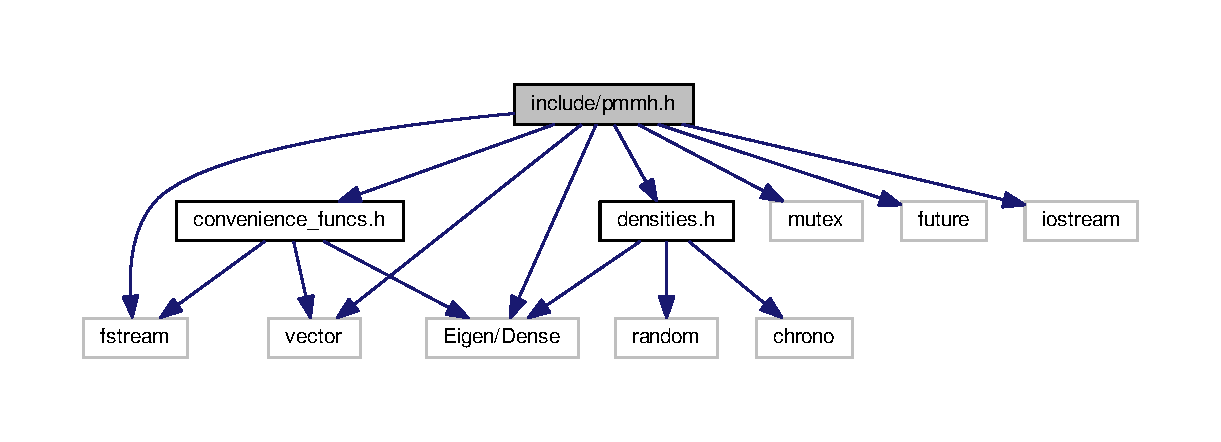
\includegraphics[width=350pt]{pmmh_8h__incl}
\end{center}
\end{figure}
\subsection*{Classes}
\begin{DoxyCompactItemize}
\item 
class \hyperlink{classPmmh}{Pmmh}
\begin{DoxyCompactList}\small\item\em A base-\/class for particle marginal Metropolis-\/\+Hastings. \end{DoxyCompactList}\end{DoxyCompactItemize}
\subsection*{Typedefs}
\begin{DoxyCompactItemize}
\item 
typedef Eigen\+::\+Matrix$<$ double, Eigen\+::\+Dynamic, 1 $>$ \hyperlink{pmmh_8h_a4c7df05c6f5e8a0d15ae14bcdbc07152}{Vec}
\item 
typedef Eigen\+::\+Matrix$<$ double, Eigen\+::\+Dynamic, Eigen\+::\+Dynamic $>$ \hyperlink{pmmh_8h_ae601f56a556993079f730483c574356f}{Mat}
\end{DoxyCompactItemize}


\subsection{Detailed Description}
A base class for particle marginal Metropolis-\/\+Hastings. Inherit from this if you want to use pmmh to estimate your S\+SM. The benefits are that doing so will force you to implement certain functions, and it will abstract away the threaded MH implementation. 



\subsection{Typedef Documentation}
\index{pmmh.\+h@{pmmh.\+h}!Mat@{Mat}}
\index{Mat@{Mat}!pmmh.\+h@{pmmh.\+h}}
\subsubsection[{\texorpdfstring{Mat}{Mat}}]{\setlength{\rightskip}{0pt plus 5cm}typedef Eigen\+::\+Matrix$<$ double, Eigen\+::\+Dynamic, Eigen\+::\+Dynamic $>$ {\bf Mat}}\hypertarget{pmmh_8h_ae601f56a556993079f730483c574356f}{}\label{pmmh_8h_ae601f56a556993079f730483c574356f}
typedef for linear algebra stuff \index{pmmh.\+h@{pmmh.\+h}!Vec@{Vec}}
\index{Vec@{Vec}!pmmh.\+h@{pmmh.\+h}}
\subsubsection[{\texorpdfstring{Vec}{Vec}}]{\setlength{\rightskip}{0pt plus 5cm}typedef Eigen\+::\+Matrix$<$ double, Eigen\+::\+Dynamic, 1 $>$ {\bf Vec}}\hypertarget{pmmh_8h_a4c7df05c6f5e8a0d15ae14bcdbc07152}{}\label{pmmh_8h_a4c7df05c6f5e8a0d15ae14bcdbc07152}
typedef for linear algebra stuff 
\hypertarget{sisr__filter_8h}{}\section{include/sisr\+\_\+filter.h File Reference}
\label{sisr__filter_8h}\index{include/sisr\+\_\+filter.\+h@{include/sisr\+\_\+filter.\+h}}


A base-\/class for Sequential Importance Sampling with Resampling. Inherit from this if you want to use a S\+I\+SR for your state space model. Filtering only; no smoothing.  


{\ttfamily \#include $<$Eigen/\+Dense$>$}\\*
{\ttfamily \#include \char`\"{}mn\+\_\+resampler.\+h\char`\"{}}\\*
Include dependency graph for sisr\+\_\+filter.\+h\+:\nopagebreak
\begin{figure}[H]
\begin{center}
\leavevmode
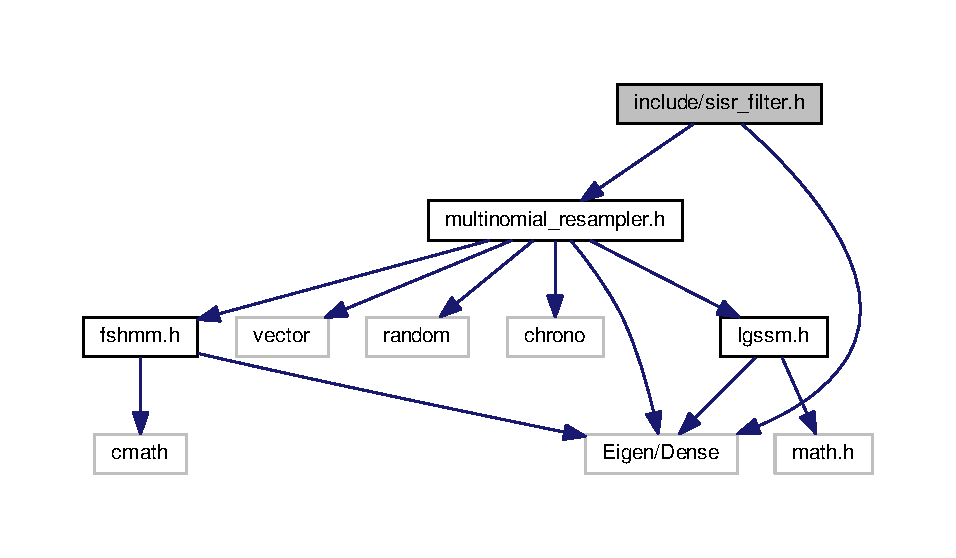
\includegraphics[width=350pt]{sisr__filter_8h__incl}
\end{center}
\end{figure}
\subsection*{Classes}
\begin{DoxyCompactItemize}
\item 
class \hyperlink{classSISRFilter}{S\+I\+S\+R\+Filter$<$ N $>$}
\begin{DoxyCompactList}\small\item\em A base-\/class for Sequential Importance Sampling with Resampling. Filtering only; no smoothing. \end{DoxyCompactList}\end{DoxyCompactItemize}
\subsection*{Typedefs}
\begin{DoxyCompactItemize}
\item 
typedef Eigen\+::\+Matrix$<$ double, Eigen\+::\+Dynamic, 1 $>$ \hyperlink{sisr__filter_8h_a4c7df05c6f5e8a0d15ae14bcdbc07152}{Vec}
\item 
typedef Eigen\+::\+Matrix$<$ double, Eigen\+::\+Dynamic, Eigen\+::\+Dynamic $>$ \hyperlink{sisr__filter_8h_ae601f56a556993079f730483c574356f}{Mat}
\end{DoxyCompactItemize}
\subsection*{Enumerations}
\begin{DoxyCompactItemize}
\item 
enum \hyperlink{sisr__filter_8h_a2486051fd2028dedca520d3e0f8fd92f}{S\+I\+S\+R\+Resamp\+Style} \{ \\*
{\bfseries everytime\+\_\+multinomial}, 
{\bfseries never}, 
{\bfseries ess\+\_\+multinomial}, 
{\bfseries everytime\+\_\+multinomial}, 
\\*
{\bfseries never}, 
{\bfseries ess\+\_\+multinomial}
 \}
\end{DoxyCompactItemize}


\subsection{Detailed Description}
A base-\/class for Sequential Importance Sampling with Resampling. Inherit from this if you want to use a S\+I\+SR for your state space model. Filtering only; no smoothing. 


\begin{DoxyTemplParams}{Template Parameters}
{\em N} & the number of particles \\
\hline
\end{DoxyTemplParams}


\subsection{Typedef Documentation}
\index{sisr\+\_\+filter.\+h@{sisr\+\_\+filter.\+h}!Mat@{Mat}}
\index{Mat@{Mat}!sisr\+\_\+filter.\+h@{sisr\+\_\+filter.\+h}}
\subsubsection[{\texorpdfstring{Mat}{Mat}}]{\setlength{\rightskip}{0pt plus 5cm}typedef Eigen\+::\+Matrix$<$ double, Eigen\+::\+Dynamic, Eigen\+::\+Dynamic $>$ {\bf Mat}}\hypertarget{sisr__filter_8h_ae601f56a556993079f730483c574356f}{}\label{sisr__filter_8h_ae601f56a556993079f730483c574356f}
typedef for linear algebra stuff \index{sisr\+\_\+filter.\+h@{sisr\+\_\+filter.\+h}!Vec@{Vec}}
\index{Vec@{Vec}!sisr\+\_\+filter.\+h@{sisr\+\_\+filter.\+h}}
\subsubsection[{\texorpdfstring{Vec}{Vec}}]{\setlength{\rightskip}{0pt plus 5cm}typedef Eigen\+::\+Matrix$<$ double, Eigen\+::\+Dynamic, 1 $>$ {\bf Vec}}\hypertarget{sisr__filter_8h_a4c7df05c6f5e8a0d15ae14bcdbc07152}{}\label{sisr__filter_8h_a4c7df05c6f5e8a0d15ae14bcdbc07152}
typedef for linear algebra stuff 

\subsection{Enumeration Type Documentation}
\index{sisr\+\_\+filter.\+h@{sisr\+\_\+filter.\+h}!S\+I\+S\+R\+Resamp\+Style@{S\+I\+S\+R\+Resamp\+Style}}
\index{S\+I\+S\+R\+Resamp\+Style@{S\+I\+S\+R\+Resamp\+Style}!sisr\+\_\+filter.\+h@{sisr\+\_\+filter.\+h}}
\subsubsection[{\texorpdfstring{S\+I\+S\+R\+Resamp\+Style}{SISRResampStyle}}]{\setlength{\rightskip}{0pt plus 5cm}enum {\bf S\+I\+S\+R\+Resamp\+Style}\hspace{0.3cm}{\ttfamily [strong]}}\hypertarget{sisr__filter_8h_a2486051fd2028dedca520d3e0f8fd92f}{}\label{sisr__filter_8h_a2486051fd2028dedca520d3e0f8fd92f}
enum class for the type of resampling to be performed 
\hypertarget{sisr__smooth_8h}{}\section{include/sisr\+\_\+smooth.h File Reference}
\label{sisr__smooth_8h}\index{include/sisr\+\_\+smooth.\+h@{include/sisr\+\_\+smooth.\+h}}


A base-\/class for Sequential Importance Sampling with Resampling. Inherit from this if you want to use a S\+I\+SR for your state space model.  


{\ttfamily \#include $<$Eigen/\+Dense$>$}\\*
{\ttfamily \#include \char`\"{}multinomial\+\_\+resampler.\+h\char`\"{}}\\*
Include dependency graph for sisr\+\_\+smooth.\+h\+:\nopagebreak
\begin{figure}[H]
\begin{center}
\leavevmode
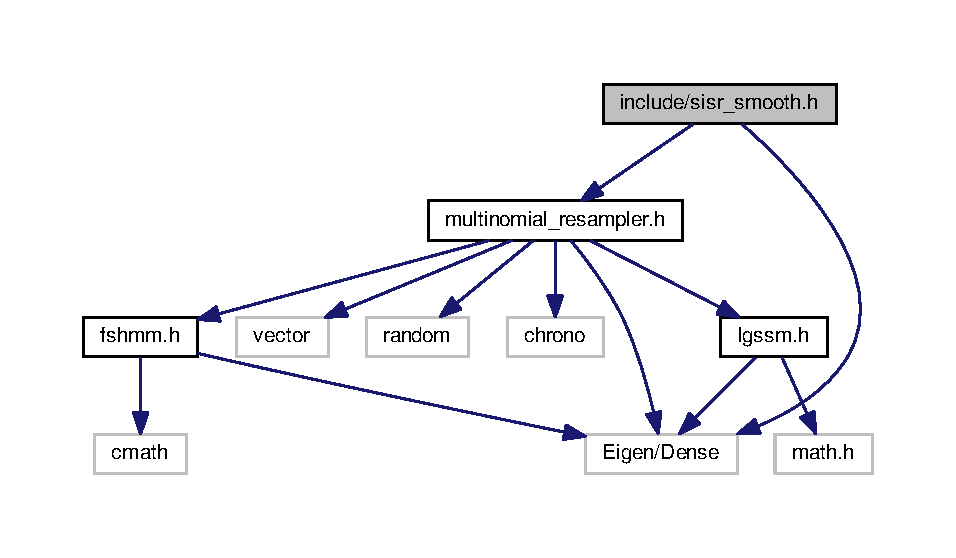
\includegraphics[width=350pt]{sisr__smooth_8h__incl}
\end{center}
\end{figure}
\subsection*{Classes}
\begin{DoxyCompactItemize}
\item 
class \hyperlink{classSISRSmoother}{S\+I\+S\+R\+Smoother}
\begin{DoxyCompactList}\small\item\em A base-\/class for Sequential Importance Sampling with Resampling. \end{DoxyCompactList}\end{DoxyCompactItemize}
\subsection*{Typedefs}
\begin{DoxyCompactItemize}
\item 
typedef Eigen\+::\+Matrix$<$ double, Eigen\+::\+Dynamic, 1 $>$ \hyperlink{sisr__smooth_8h_a4c7df05c6f5e8a0d15ae14bcdbc07152}{Vec}
\item 
typedef Eigen\+::\+Matrix$<$ double, Eigen\+::\+Dynamic, Eigen\+::\+Dynamic $>$ \hyperlink{sisr__smooth_8h_ae601f56a556993079f730483c574356f}{Mat}
\end{DoxyCompactItemize}
\subsection*{Enumerations}
\begin{DoxyCompactItemize}
\item 
enum \hyperlink{sisr__smooth_8h_a2486051fd2028dedca520d3e0f8fd92f}{S\+I\+S\+R\+Resamp\+Style} \{ \\*
{\bfseries everytime\+\_\+multinomial}, 
{\bfseries never}, 
{\bfseries ess\+\_\+multinomial}, 
{\bfseries everytime\+\_\+multinomial}, 
\\*
{\bfseries never}, 
{\bfseries ess\+\_\+multinomial}
 \}
\end{DoxyCompactItemize}


\subsection{Detailed Description}
A base-\/class for Sequential Importance Sampling with Resampling. Inherit from this if you want to use a S\+I\+SR for your state space model. 



\subsection{Typedef Documentation}
\index{sisr\+\_\+smooth.\+h@{sisr\+\_\+smooth.\+h}!Mat@{Mat}}
\index{Mat@{Mat}!sisr\+\_\+smooth.\+h@{sisr\+\_\+smooth.\+h}}
\subsubsection[{\texorpdfstring{Mat}{Mat}}]{\setlength{\rightskip}{0pt plus 5cm}typedef Eigen\+::\+Matrix$<$ double, Eigen\+::\+Dynamic, Eigen\+::\+Dynamic $>$ {\bf Mat}}\hypertarget{sisr__smooth_8h_ae601f56a556993079f730483c574356f}{}\label{sisr__smooth_8h_ae601f56a556993079f730483c574356f}
typedef for linear algebra stuff \index{sisr\+\_\+smooth.\+h@{sisr\+\_\+smooth.\+h}!Vec@{Vec}}
\index{Vec@{Vec}!sisr\+\_\+smooth.\+h@{sisr\+\_\+smooth.\+h}}
\subsubsection[{\texorpdfstring{Vec}{Vec}}]{\setlength{\rightskip}{0pt plus 5cm}typedef Eigen\+::\+Matrix$<$ double, Eigen\+::\+Dynamic, 1 $>$ {\bf Vec}}\hypertarget{sisr__smooth_8h_a4c7df05c6f5e8a0d15ae14bcdbc07152}{}\label{sisr__smooth_8h_a4c7df05c6f5e8a0d15ae14bcdbc07152}
typedef for linear algebra stuff 

\subsection{Enumeration Type Documentation}
\index{sisr\+\_\+smooth.\+h@{sisr\+\_\+smooth.\+h}!S\+I\+S\+R\+Resamp\+Style@{S\+I\+S\+R\+Resamp\+Style}}
\index{S\+I\+S\+R\+Resamp\+Style@{S\+I\+S\+R\+Resamp\+Style}!sisr\+\_\+smooth.\+h@{sisr\+\_\+smooth.\+h}}
\subsubsection[{\texorpdfstring{S\+I\+S\+R\+Resamp\+Style}{SISRResampStyle}}]{\setlength{\rightskip}{0pt plus 5cm}enum {\bf S\+I\+S\+R\+Resamp\+Style}\hspace{0.3cm}{\ttfamily [strong]}}\hypertarget{sisr__smooth_8h_a2486051fd2028dedca520d3e0f8fd92f}{}\label{sisr__smooth_8h_a2486051fd2028dedca520d3e0f8fd92f}
enum class for the type of resampling to be performed 
%--- End generated contents ---

% Index
\backmatter
\newpage
\phantomsection
\clearemptydoublepage
\addcontentsline{toc}{chapter}{Index}
\printindex

\end{document}
